\documentclass{EPSA-rap-template}

\usepackage{pdfpages}
\usepackage{eurosym}

\usepackage{tocloft}

\type{Abaque}

\titresize{\large} % ne pas hésiter a changer la taille :
%\normalsize
%\large
%\Large
%\LARGE
%\huge
%\Huge
%\HUGE

\titre{ Liste des composants électronique Standard EPSA}
\titresh{Composants Standard } % Titre réduit pour les en-tête et bas de page

\departement{BASTIE et CHAIPE}
\departementsh{Elec}% Département réduit pour les en-tête et bas de page

\auteurs{Eymeric \textbf{Chauchat}}

\version{V2}

\versionnement{
\ver{V2}{18 Octobre 2022}{ECT}{Forme Finale V2.}{4} \\
\ver{V1.5}{17 Octobre 2022}{ECT}{Finalisation de la liste de composants.}{3} \\
\ver{V1.0}{2 Octobre 2022}{ ECT }{Rédaction initiale.}{1}
}

\addtolength{\cftsecnumwidth}{15pt}
\addtolength{\cftsubsecnumwidth}{15pt}
\addtolength{\cftsubsubsecnumwidth}{15pt}

\setuppack

\newcommand{\includepdfscale}{0.84}

\begin{document}

\fairepagedegarde
\newpage
\tableofcontents

\newpage

\section{Introduction}

Lors de la création de cartes électroniques au sein de l'EPSA uniquement une liste de composants standard est autorisé (hormis dérogation pour carte spécifique). Cette liste doit être actualisée chaque année par le Directeur du département BASTIE.

Cette démarche permet de simplifier grandement la logistique concernant les cartes électroniques et permet d'avoir une politique long terme des cartes électroniques. Aucun achat d'un composant supplémentaire sans avoir concerté le directeur technique, le directeur BASTIE et le directeur Chaipe ne sera toléré. Cette liste permet de restreindre le nombre de boitier de composant

\section{Résistance}

A l'EPSA nous avons avoir l'usage de deux types de résistances : les résistances à valeur fixe et les résistances variable. Les résistance variables sont faite pour rajouter un réglage sur une carte (capteur de tension etc).

\subsection{Résistance à usage générale}

Toutes les résistances proviennent du cahier de résistance \href{https://fr.farnell.com/multicomp-pro/mp003365/kit-resi-0r-1m-0-25w-1-1206-9900pc/dp/3405258}{ MP003365  de la marque MultiComp}. Les résistances sont des CMS de la taille 1206 et les valeurs permises sont celle trouvables dans \hyperlink{ResTab}{le tableau des résistances}. Leur tension nominal est de 200V et sont conçues pour un quart de Watt, \textbf{Attention alors quand on design une carte pour les capteurs haute tension}

\subsection{Résistance variable (triming Potentiometer)}

Nous utiliserons \hyperlink{DataSheetTrim}{les Trimming Potentiometer BOURNS 3296Y} (Y est la forme du boitier). Elles ont 25 tours de réglages nominale, 0.5W nominal et 250V nominal. La valeur des résistances disponibles est la suivante :

\begin{itemize}
\item 200 \Omega
\item 20 k \Omega
\item 200 k \Omega
\item 1 M \Omega
\end{itemize}

Plus spécifiquement ces potentiomètres permettent de faire instantanément un pont diviseur de tension en utilisant les deux côtés de la résistance.

\section{Condensateurs}

Tous les condensateurs proviennent de la boite de condensateur \href{https://fr.farnell.com/wurth-elektronik/885070/kit-condensateur-ceram-multicouche/dp/2491608}{885070 de chez Wurth Elektronik}. Les condensateur sont des CMS de la taille 0805 et les valeurs permises sont celle trouvable dans \hyperlink{CapTab}{le tableau des condensateur}

\section{Timer et dérivée 555}

Pour permettre de compter le temps ou de créer des circuits clignotants nous utilisons à l'EPSA la puce 555 (de ses noms complets NE555,SE555 ou LM555) en version CMS (Composants montée en surface). Les variantes des composants 555 sont interchangeables entre eux et prennent tous la même place sur carte. On peut retrouver en annexe \hyperlink{555}{Les deux applications standards} du circuit 555 (permettant de générer une horloge (Astable) ou une pulse de durée minimal fixé (Monostable) ).

L'encapsulation choisi est SOIC-8. La référence complète choisi cette année est LM555CMX/NOPB.



\section{Comparateur de Tension}

Nous allons utilisé deux références de comparateurs de tension différentes : les comparateurs simple et les comparateurs double. Les comparateurs simple permettent de comparer une tension par rapport à une autre. Les doubles peuvent servir d'encadrer une tension ou d'exclure une plage de tension .

Les comparateurs possèdent des sorties à collecteur ouvert il faut donc utiliser une résistance de tirage a la sortie pour obtenir une tension à la sortie.

\subsection{Comparateur Simple}

Nous utilisons les comparateurs de tension \hyperlink{Comparateur}{TS391 de STelectronics}. Ce sont principalement ce qu'on peut appeler des amplis opérationnels.

Ils existent en deux configurations : ILT (la version IYLT possède uniquement une coque vérifiant d'autre norme) et RILT (R pour Right) nous avons choisi la ILT. Nous pouvons retrouver en annexe \hyperlink{AmpliOp}{le schéma de câblage des comparateurs }

L'encapsulation utilisé comme pour les portes logiques est le SOT23-5.

\subsection{Comparateur double}

Nous utilisons \hyperlink{ComparateurDouble}{ les comparateurs à deux entrées LM393LV-Q1 } de chez Texas instrument. Ils fonctionnent comme les comparateurs simple sauf qu'il y en a deux dans le même boitier.

L'encapsulation utilisé est le format SOIC-8

\section{Alimentation Régulé}

Une des parties principales d'un circuit (qu'il ne faut jamais négliger) est son alimentation. Nous avons besoin à l'EPSA d'une alimentation 12V-5V et d'une alimentation d'isolation 5V-5V (pour permettre l'isolation galvanique du circuit). Nous avons choisi dans les deux cas d'utiliser des alimentations à découplage. Elles sont plus chère que des alimentations linéaires (qui "brulent" la tension en trop) mais permettent de gagner des points sur l'épreuve de Design et de vider moins les batteries.

\subsection{Alimentation abaisseur de tension}

Nous avons choisi d'utiliser deux alimentations différentes la \hyperlink{Alim}{ TSR 2-2450 et la TSR 0.5-2450  de chez Traco Power }. Les deux possèdent le même encombrement sur les cartes mais l'une possède un courant nominal de sortie de 2A et l'autre de 0.5A. (question de prix)

% TSR 2-2450 Traco Power regulateur 36V - 5V
% TSR 0.5-2450 


\subsection{Alimentation d'isolation}

L'alimentation d'isolation 5V-5V qui a été choisi est la \hyperlink{AlimIsol}{PDME2-S5-S5-S5 de chez CUI INC}. Elle possède une isolation galvanique de 1.5kV (EV 4.3.6). L'utilisation de cette isolation est très simple il suffit de lui fournir une tension en entrée et elle fournit une tension en sortie. Des Condensateurs peuvent être rajouté en entrée et en sorti pour stabiliser encore plus les sources de tensions (voir le \hyperlink{IsolAlim}{schéma de branchement de l'alimentation isolé})

%On utilise une diode TLS pour contrer les réponses transitoires potentiel de la batterie (pic de tension) SMBJ28A-Q MGQ.

\section{ Porte Logique }

Pour fabriquer des cartes à l'EPSA nous devons utiliser des portes logiques (AND, OR , XOR et NOT). Elles sont encapsulé dans le format SOT23-5. Contrairement au comparateur elle ne sont pas en sortie à collecteur ouverte. Dans ce cas lier deux outputs de porte logique ensemble créera un cour-circuit.

Nous avons choisi les portes logiques SN74AHCT1G de chez Texas instrument.

Voici la liste complète des références : 
\begin{itemize}
\item \hyperlink{And}{AND : SN74AHCT1G08DBVR}
\item \hyperlink{Or}{OR : SN74AHCT1G32DBVR}
\item \hyperlink{NAnd}{NAND : SN74AHCT1G00DBVR}
\item \hyperlink{NOr}{NOR : SN74AHCT1G02DBVR}
\item \hyperlink{XOr}{XOR : SN74AHCT1G86DBVR}
\end{itemize}

\section{Opto-coupleur}

Pour permettre le transport isolé galvaniquement d'une information, nous utilisons des opto-coupleurs (coupleur optique) aussi appelé des solid state relay (SSR). Nous avons choisi les \hyperlink{SSR}{CPC1394 de chez IXYS}, ils permettent une isolation galvanique de 5kV, une commutation de 600V et une intensité de commutation aux alentours de 4mA. Nous pouvons ainsi les utiliser en sortie de porte logique. 

L'encapsulation est en DIP-4.

\section{Bascule D}

La bascule D nous permet de créer des verrous sur nos cartes (la plupart du temps une protection qui s'installe lors d'une erreur et qui s'enlève uniquement après le redémarrage total du système). Nous avons choisi la puce \hyperlink{DLatch}{SN74HCS72QDRQ1 de chez Texas Instruments}. C'est une bascule D assez volumineuse mais qui possède des fonctionnalités qui simplifie son utilisation dans notre contexte.

\section{Diode}

Nous avons besoin de diode au sein de nos cartes électroniques.
Nous avons choisi une diode classique bloquante dans un sens. Elle nous permet d'écrêter des signaux et d'éviter les branchements inverses (mais il est préférable d'utiliser un NMOS). Nous avons choisi la diode \hyperlink{Diode}{RFN1VWM2STF de chez ROHM Semiconductor}. Elle a la taille d'une capacité, laisse passer au maximum 1A et bloque une tension de 200V maximum.

\section{Mosfet}

Les mosfet sont des interrupteurs asservis électriquement. Ils nous permettent dans nos montages de commander l'allumage d'une led, d'une partie d'un circuit ou de prévenir les branchement inverse. Le mosfet de type N est le \hyperlink{NMOS}{ SQ2348ES de chez Vishay} et le mosfet de type P est le \hyperlink{PMOS}{ Si2343CDS de chez Vishay}. Les deux mosfets ont un courant continue de ligne de 4A et de 30V. Leur résistance interne à 10V est de 50 m \Omega permettant une chute de tension négligeable pour nos applications .

L'encapsulation est en SOT-23.

\section{Diode Zener}

BZX8450-C3V0-QR

BZY55B2V7 RBG mieux

TZM5224B-GS08 encore mieux

Model
[BZT52C2V4]
*SRC=BZT52C2V4;DI_BZT52C2V4;Diodes;Zener <=10V; 2.40V  0.500W   Diodes Inc. 
*SYM=HZEN
.SUBCKT DI_BZT52C2V4  1 2
*        Terminals    A   K
D1 1 2 DF
DZ 3 1 DR
VZ 2 3 0
.MODEL DF D ( IS=85.8p RS=37.1 N=1.10
+ CJO=461p VJ=0.750 M=0.330 TT=50.1n )
.MODEL DR D ( IS=17.2f RS=84.5 N=3.00 )
.ENDS

\section{Connecteur}

A l'EPSA nous utilisons des connecteurs \href{https://www.mouser.fr/c/connectors/headers-wire-housings/?contact\%20gender=Pin\%20\%28Male\%29&contact\%20plating=Gold&m=Molex&mating\%20post\%20length=7.49\%20mm&mounting\%20angle=Straight&number\%20of\%20rows=1\%20Row&pitch=2.54\%20mm&termination\%20post\%20length=3.56\%20mm&type=Locking}{Molex KK avec blocage}. Contrairement aux autres composants il peut être demandé de commander un connecteur avec un nombre de socket spécifique tant qu'il fait parti de la gamme KK ci-dessus. Les pins males sont de la série 6373 pour les droits et 171857 (7478 pour 3P) pour les angles. Les connecteurs sont de la série 2695.  Nous avons pour le moment en stock les suivants :



\begin{itemize}
\item 2 Pins 22-11-2022 (droit) 171857-4002 (angle) 22-01-3027 (connecteur)
\item 3 Pins 22-11-2032 (droit) 22-12-2034 (angle) 22-01-3037 (connecteur)
\item 4 Pins 22-11-2042 (droit) 171857-4004 (angle) 22-01-3047 (connecteur)
\item 6 Pins 22-11-2062 (droit) 171857-4006 (angle) 22-01-3067 (connecteur)
\end{itemize}

\section{Annexes}

\subsection{Liste de tous les composants}

Voici la liste de tout les composants électroniques utilisable cette année à l'EPSA :

{
\centering
\noindent
\footnotesize
\renewcommand*{\arraystretch}{1.3}
\begin{tabular}{lllll}
Fonction & Référence & Boitier & Prix unitaire & Stock recommandé \\
Résistance & MP003365 & & 197,33 \euro{} & 1 \\
200 \Omega Trim & 3296Y-1-201LF & 3296Y & 2,43  \euro{} & 10 \\
20 k\Omega Trim & 3296Y-1-203LF & 3296Y & 2,38  \euro{} & 10 \\
200 k\Omega Trim & 3296Y-1-204LF & 3296Y & 2,43  \euro{} & 10 \\
1 M\Omega Trim & 3296Y-1-105LF & 3296Y & 2,43  \euro{} & 10 \\
Condensateur & 885070 & & 178,72 \euro{} & 1 \\
Timer 555 & LM555CMX/NOPB & SOIC-8 & 1,19 \euro{} & 10 \\
Comparateur Simple & TS391ILT & SOT-23-5 & 0,87 \euro{} & 20 \\
Comparateur Double & LM393LVQDRQ1 & SOIC-8 & 0,62 \euro{} & 10 \\
Alimentation HP & TSR 2-2450 & SIP-3 & 11,10 \euro{} & 2 \\
Alimentation LP & TSR 0.5-2450 & DIP-10 & 5,20 \euro{} & 2 \\
Alimentation Isolé & PDM2-S5-S5-S & & 5,97 \euro{} & 2 \\
Porte ET & SN74AHCT1G08DBVR & SOT-23-5 & 0,49 \euro{} & 10 \\
Porte OU & SN74AHCT1G32DBVR & SOT-23-5 & 0,40 \euro{} & 10 \\
Porte NAND & SN74AHCT1G00DBVR & SOT-23-5 & 0,40 \euro{} & 10 \\
Porte NOR & SN74AHCT1G02DBVR & SOT-23-5 & 0,40 \euro{} & 10 \\
Porte XOR & SN74AHCT1G86DBVR & SOT-23-5 & 0,54 \euro{} & 10 \\
SSR & CPC1394GRTR & SMD DIP-4 & 2,36 \euro{} & 10 \\
Bascule D & SN74HCS72QDRQ1 & SOIC-14 & 0,65 \euro{} & 10 \\
Diode & RFN1VWM2STF & PMDE-2 & 0,68 \euro{} & 10 \\
NMOS & SQ2348ES-T1-BE3 & SOT-23-5 & 0,70 \euro{} & 10 \\
PMOS & SI2343CDS-T1-BE3 & SOT-23-5 & 0,65 \euro{} & 10 \\
\end{tabular}
}

\subsection{Taille CMS}

Voici le tableau des tailles de CMS

{
\centering
\begin{tabular}{cllll}
Type &	Longueur & Largeur & Hauteur  & Métallisation  \\
& L & l &H min-max   & M min-max \\
0402 &	1,00 &  0,50 &	0,50 &  \\	 
0603 & 	1,60 & 	0,80 & 	0,80 & \\	 
0805 &	2,00 &	1,25 &	0,6 ou 0,85 ou 1,25 & 0,25-0,75 \\
1206 &	3,20 &	1,60 &	0,85 ou 1,15 ou 1,6 &	0,3-1,0 \\
1210 &	3,20 &	2,50 &	1,15 ou 1,35 ou 1,8 ou 2,5 &	0,3-1,0\\
1812 &	4,50 & 	3,20 &	2,0 max &	0,3-1,0\\
2220 &	5,70 &	5,00 &	2,0 max &	0,3-1,0\\
\end{tabular}

\par
}


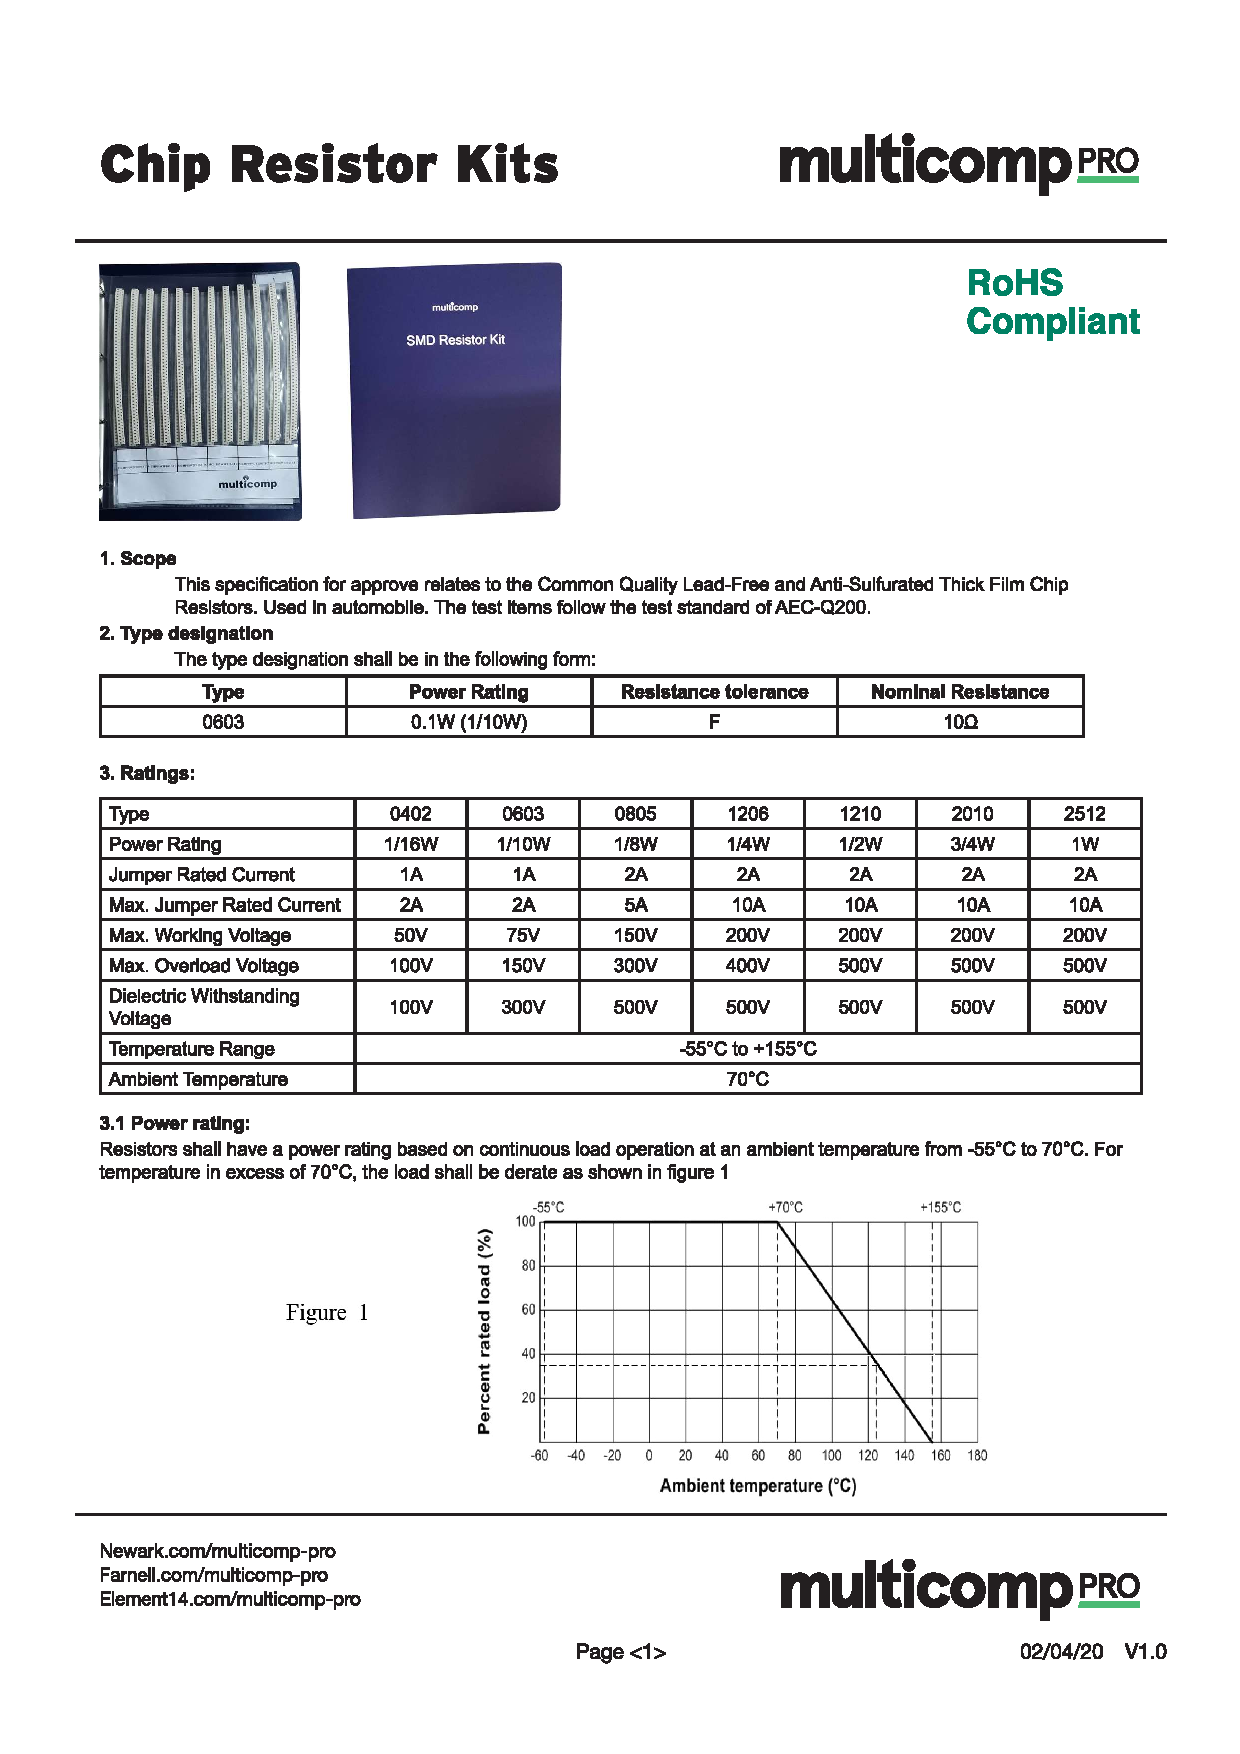
\includepdf[pages=1,scale=\includepdfscale,pagecommand={\subsection{Datasheet Resistance Générale}}]{Resistance.pdf}

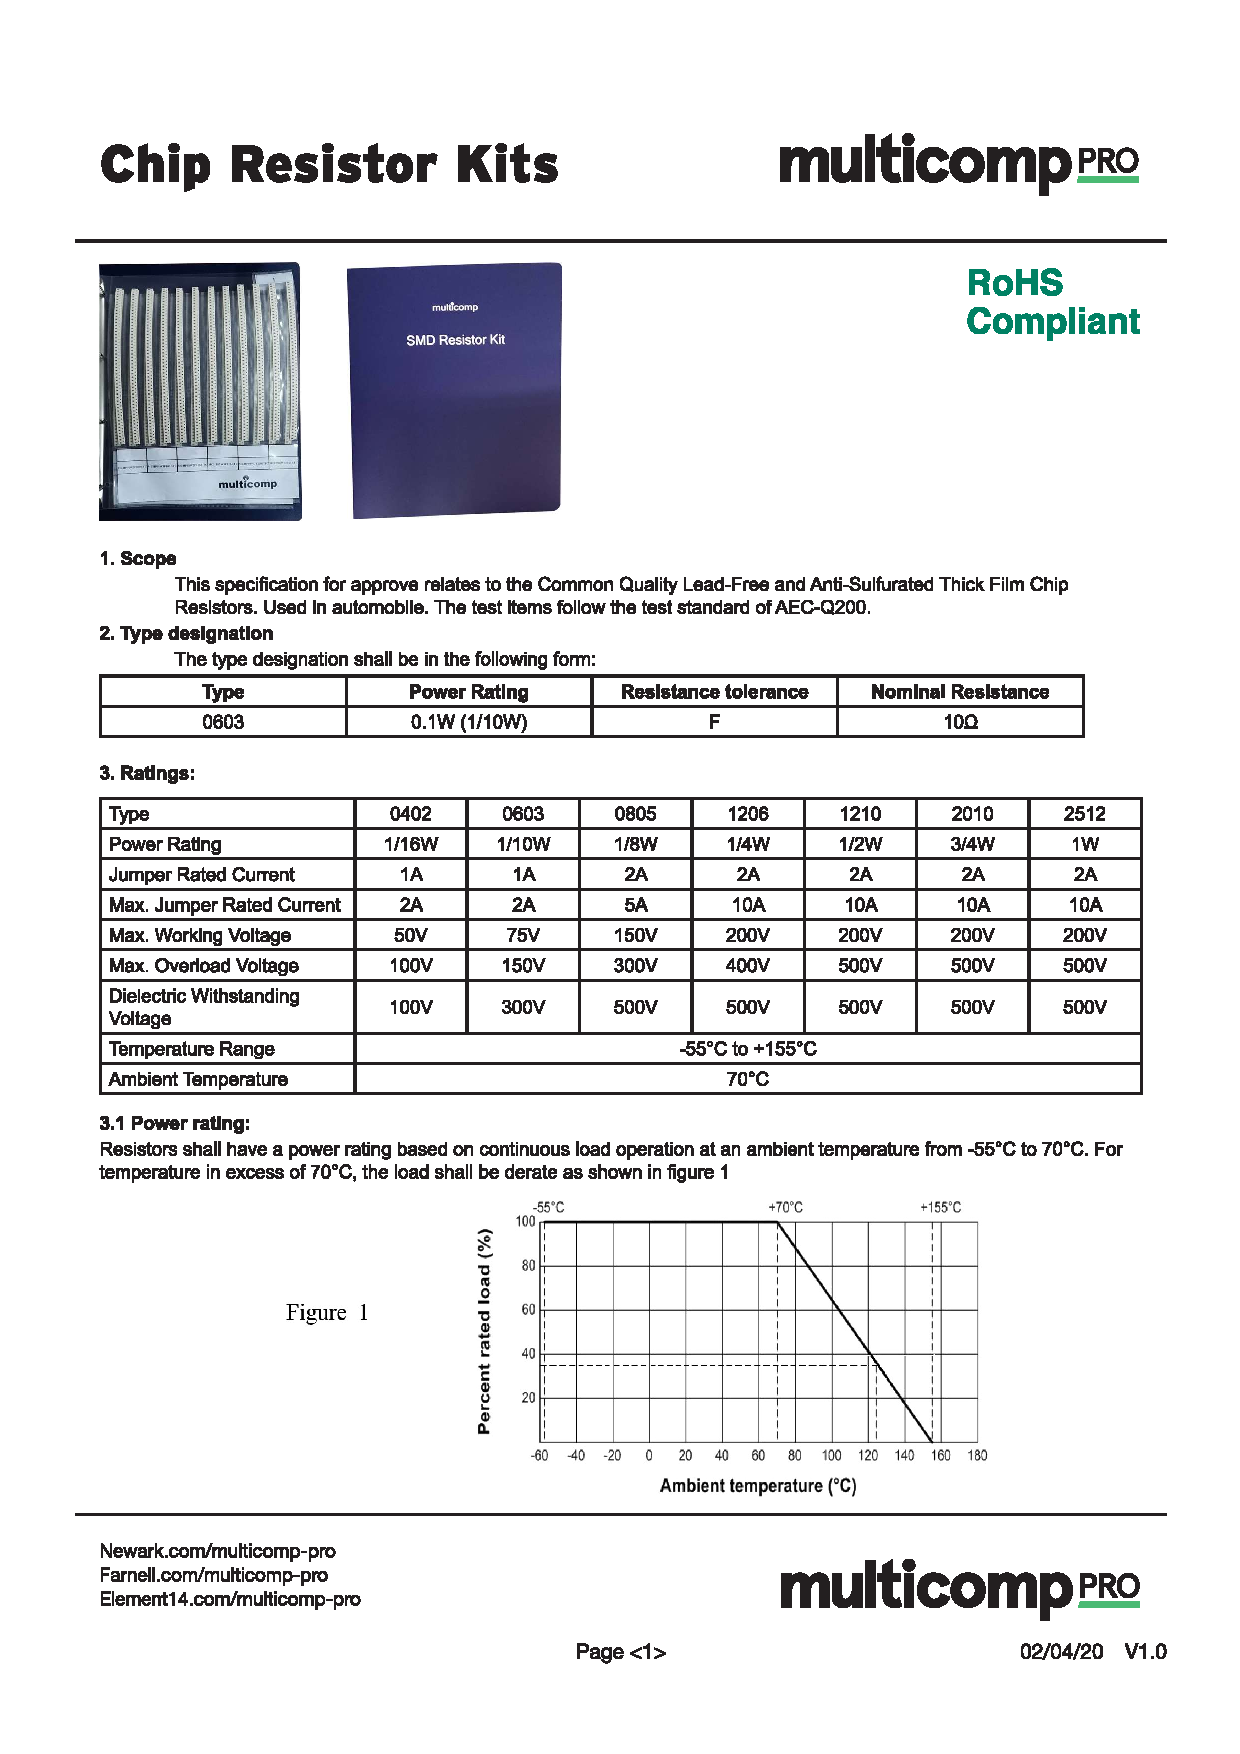
\includepdf[page=2-5,scale=\includepdfscale,pagecommand={ }]{Resistance.pdf}

\includepdf[pages=6,scale=\includepdfscale,pagecommand={\hypertarget{ResTab}{}}]{Resistance.pdf}

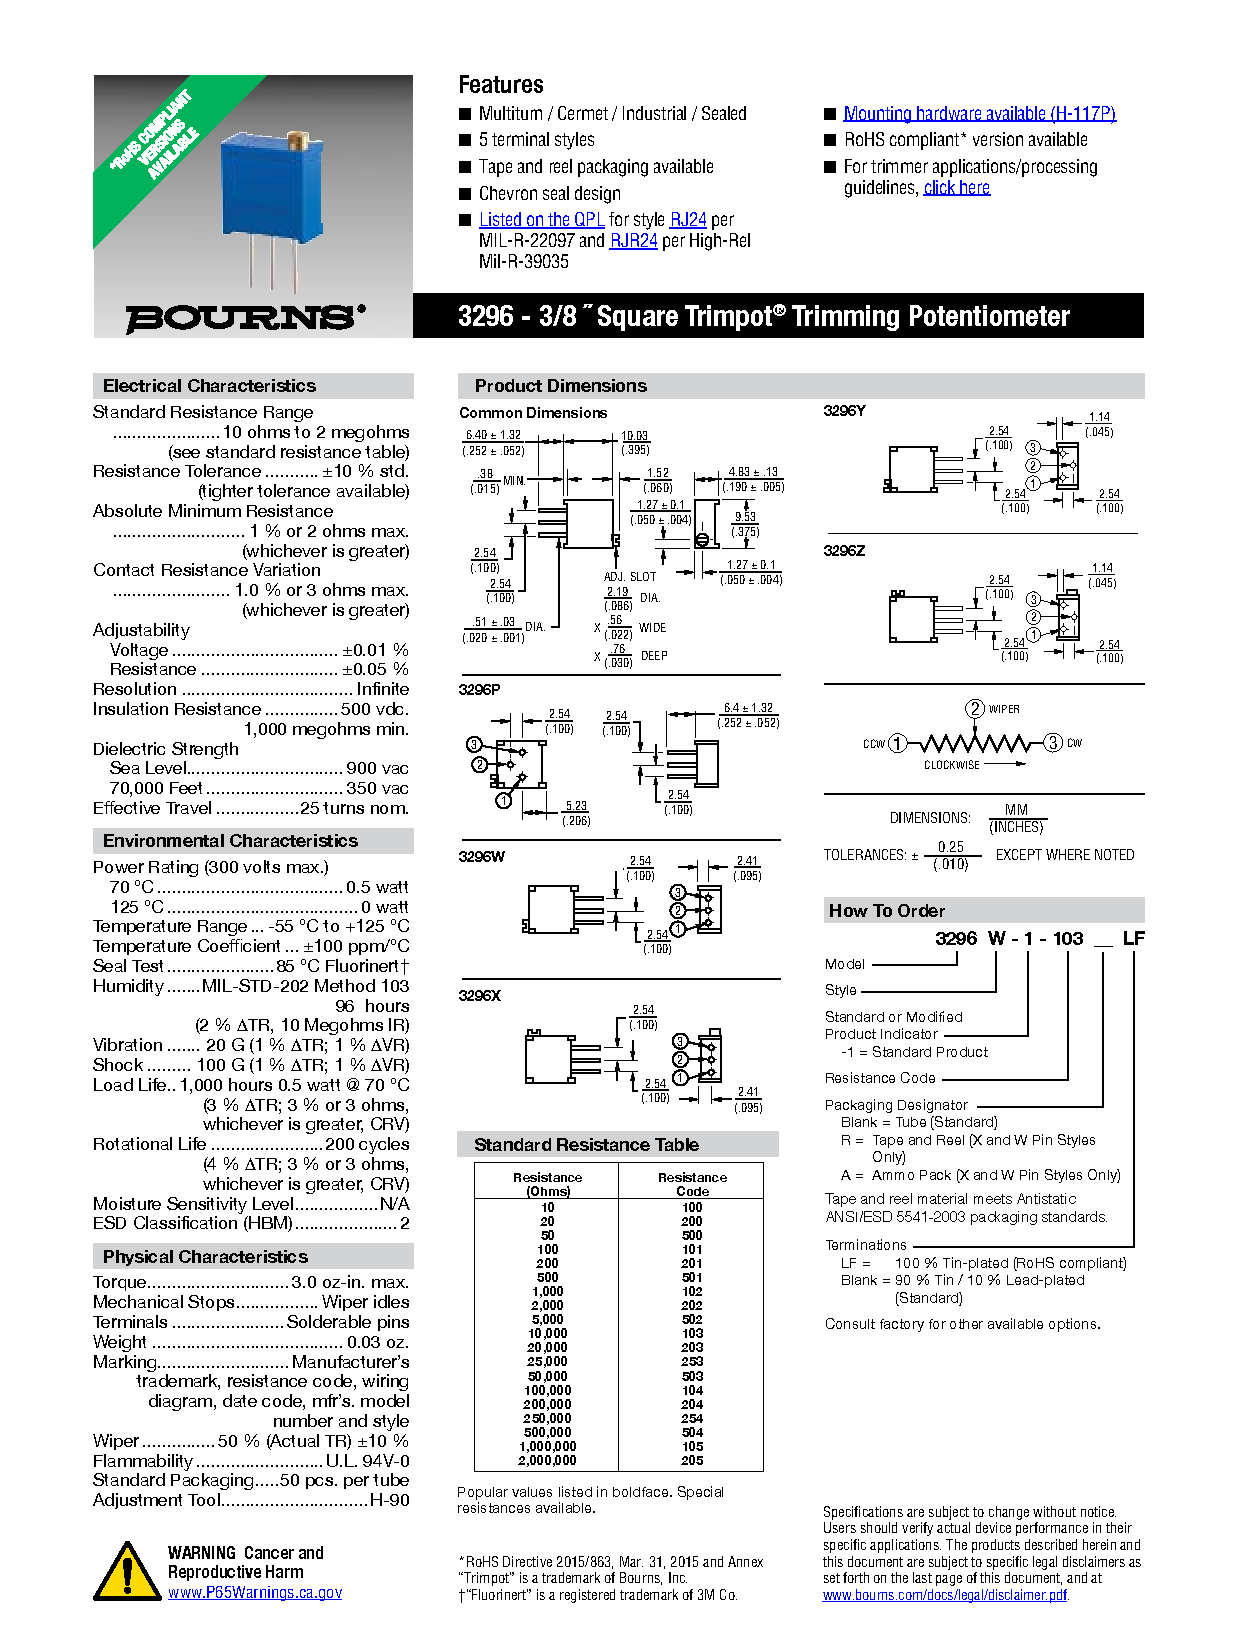
\includepdf[pages=1,scale=\includepdfscale,pagecommand={\subsection{Datasheet Resistance Variable}\hypertarget{DataSheetTrim}{}}]{Resistance variable.pdf}

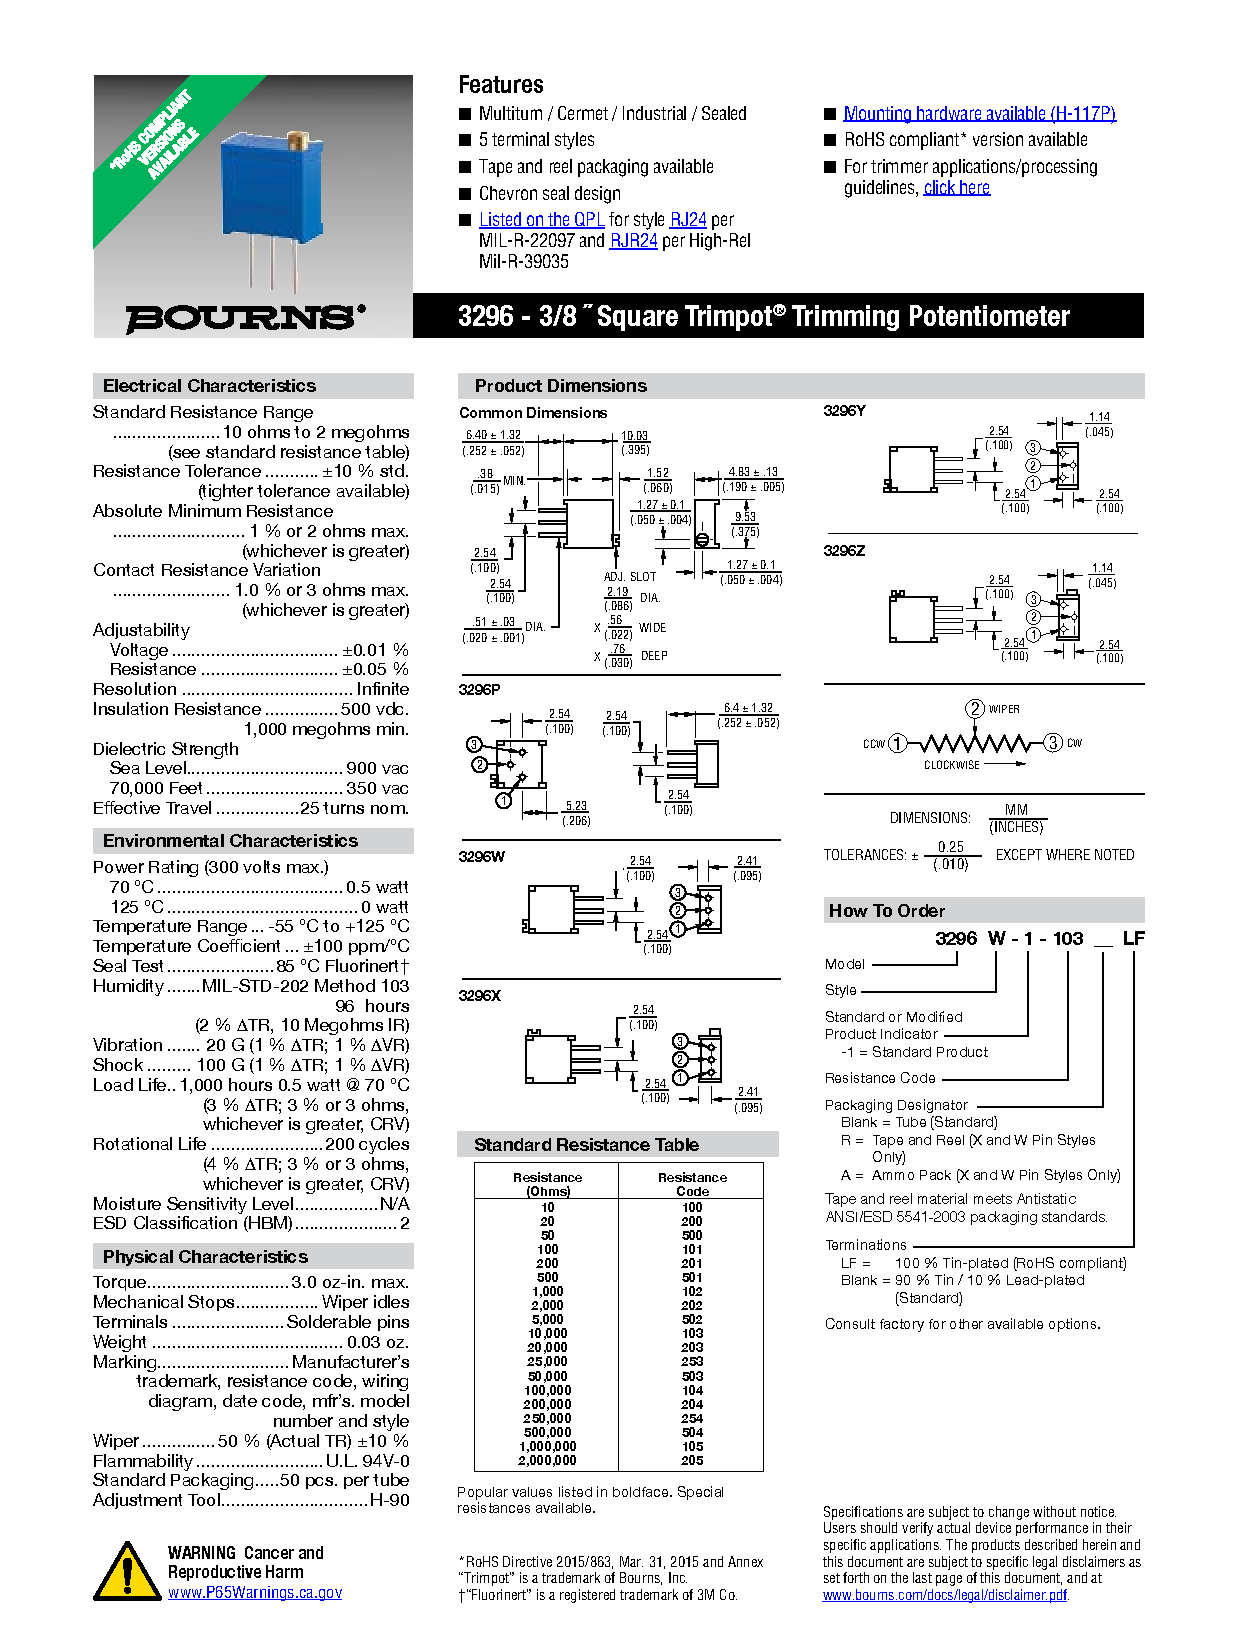
\includepdf[page=2,scale=\includepdfscale,pagecommand={ }]{Resistance variable.pdf}

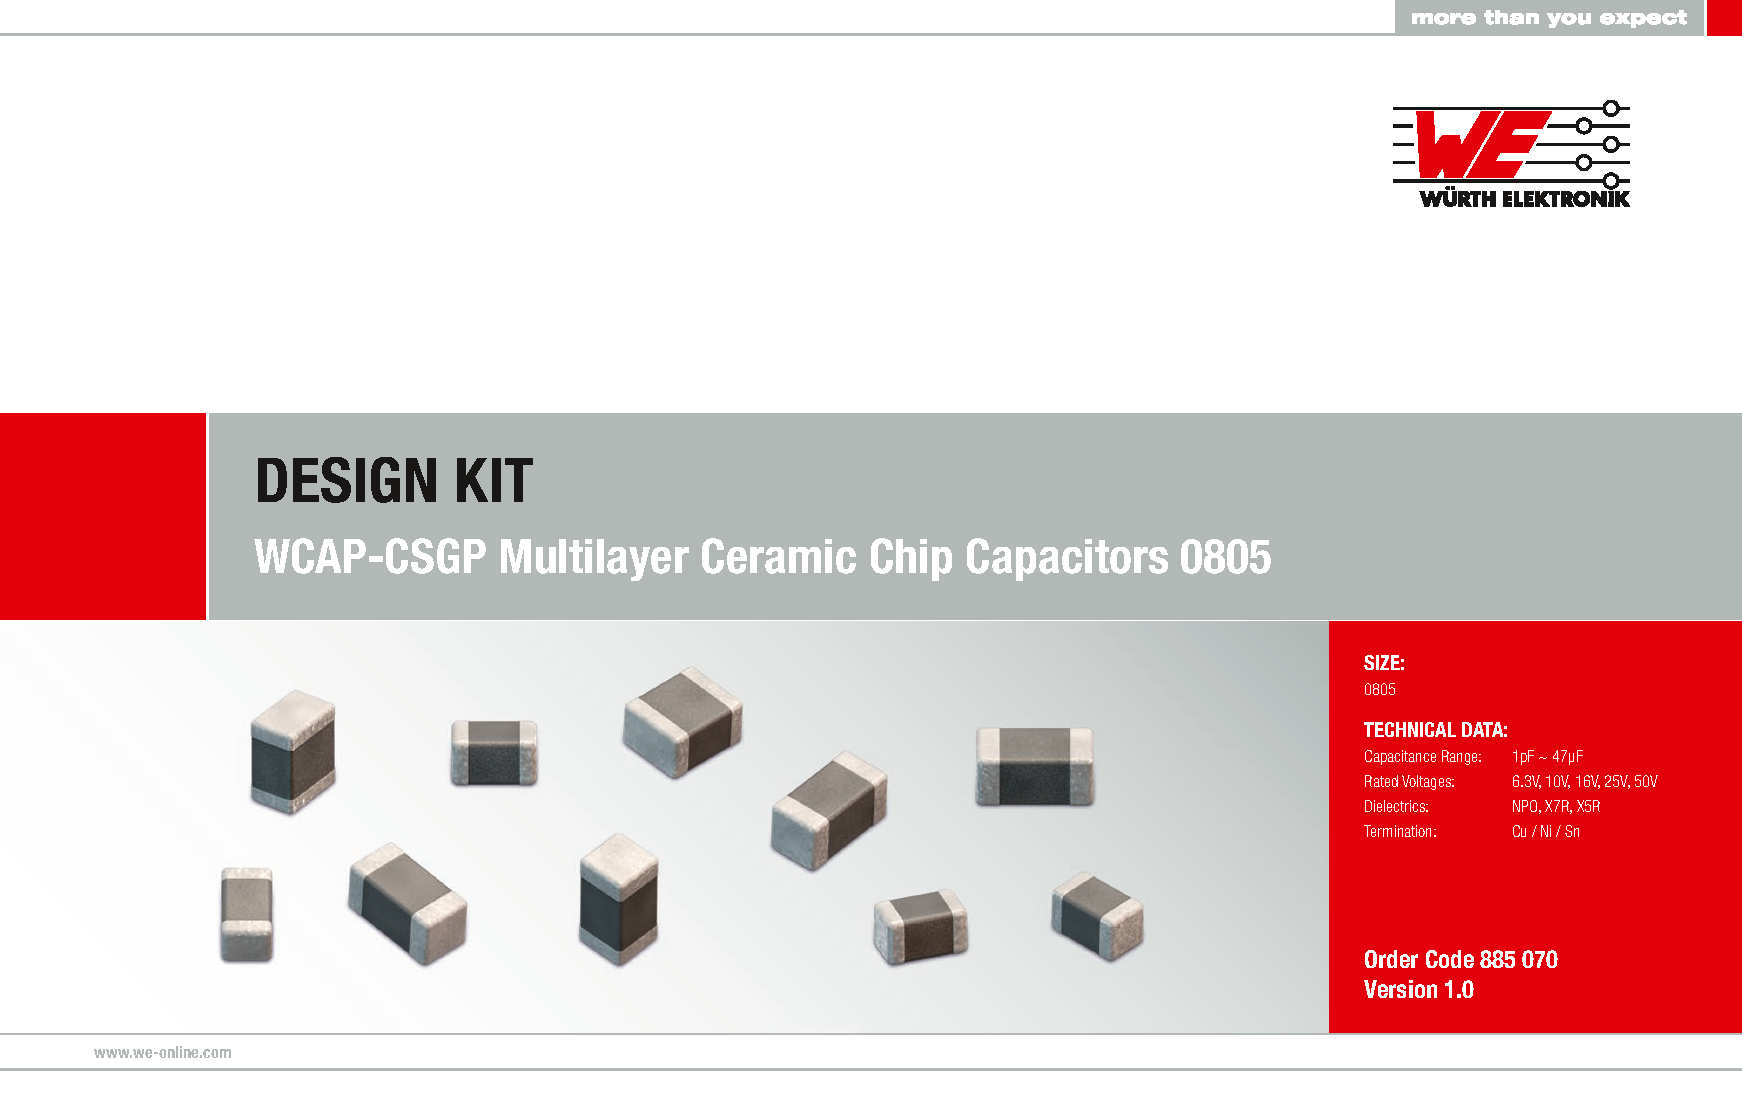
\includepdf[page=2,scale=1,pagecommand={
\subsection{Datasheet Condensateur}
{
\noindent Les valeurs sont les suivantes : 
\\
\phantom{a}
\\
\noindent \begin{tabular}{cccccccccc}
1pF & 1.5pF & 2.2pF & 3.3pF & 4.7pF & 6.8pF & 10pF & 15pF \\ 22pF & 33pF & 47pF & 68pF & 100pF & 150pF & 150pF & 220pF \\
330pF & 470pF & 680pF & 1nF & 1.5nF & 2.2nF & 3.3nF & 4.7nF \\
6.8nF & 10nF & 15nF & 22nF & 33nF & 47nF & 68nF & 100nF \\
150nF & 220nF & 330nF & 470nF & 680nF & 1$\mu$F & 2.2$\mu$F & 3.3$\mu$F \\
4.7$\mu$F & 10$\mu$F & 22$\mu$F & 47$\mu$F \\
\end{tabular}}
\hypertarget{CapTab}{}}
]{Condensateur.pdf}

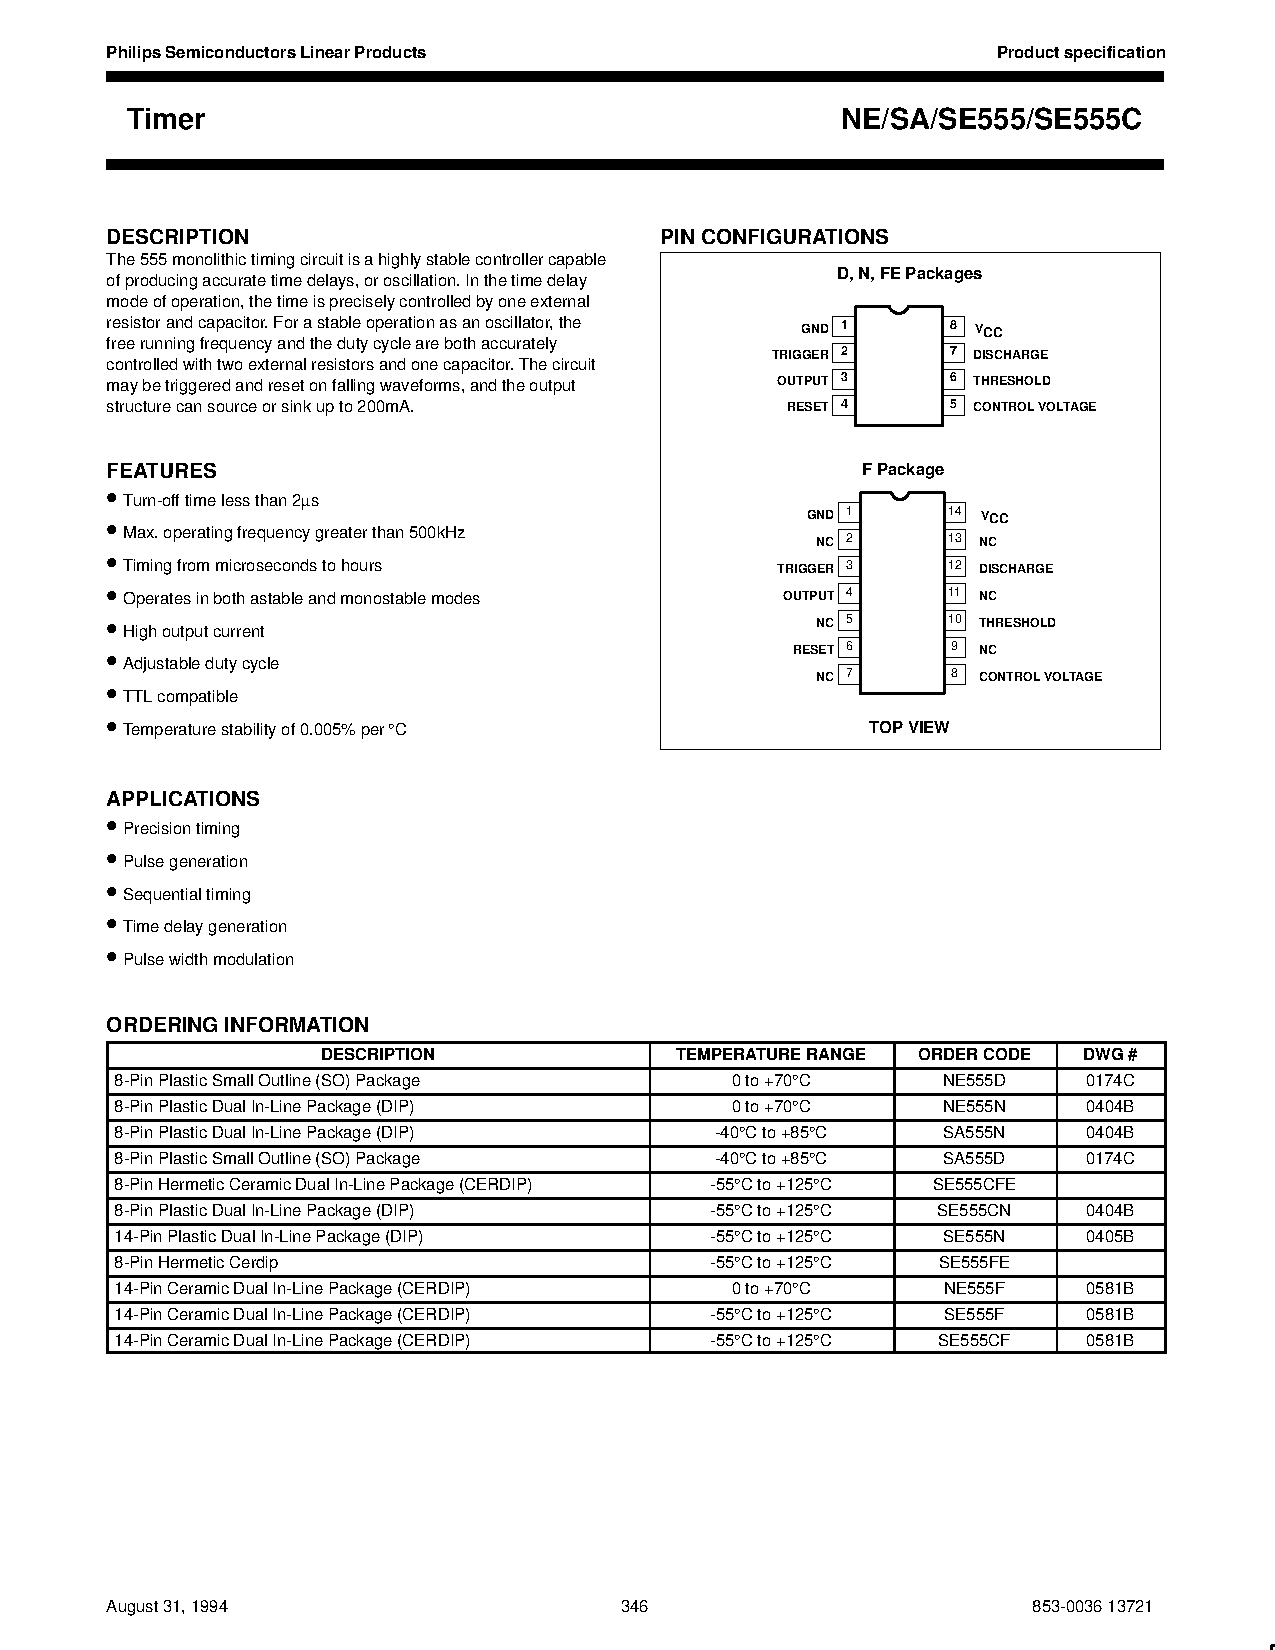
\includepdf[page=1,scale=\includepdfscale,pagecommand={\subsection{555 Datasheet}}]{555.pdf}

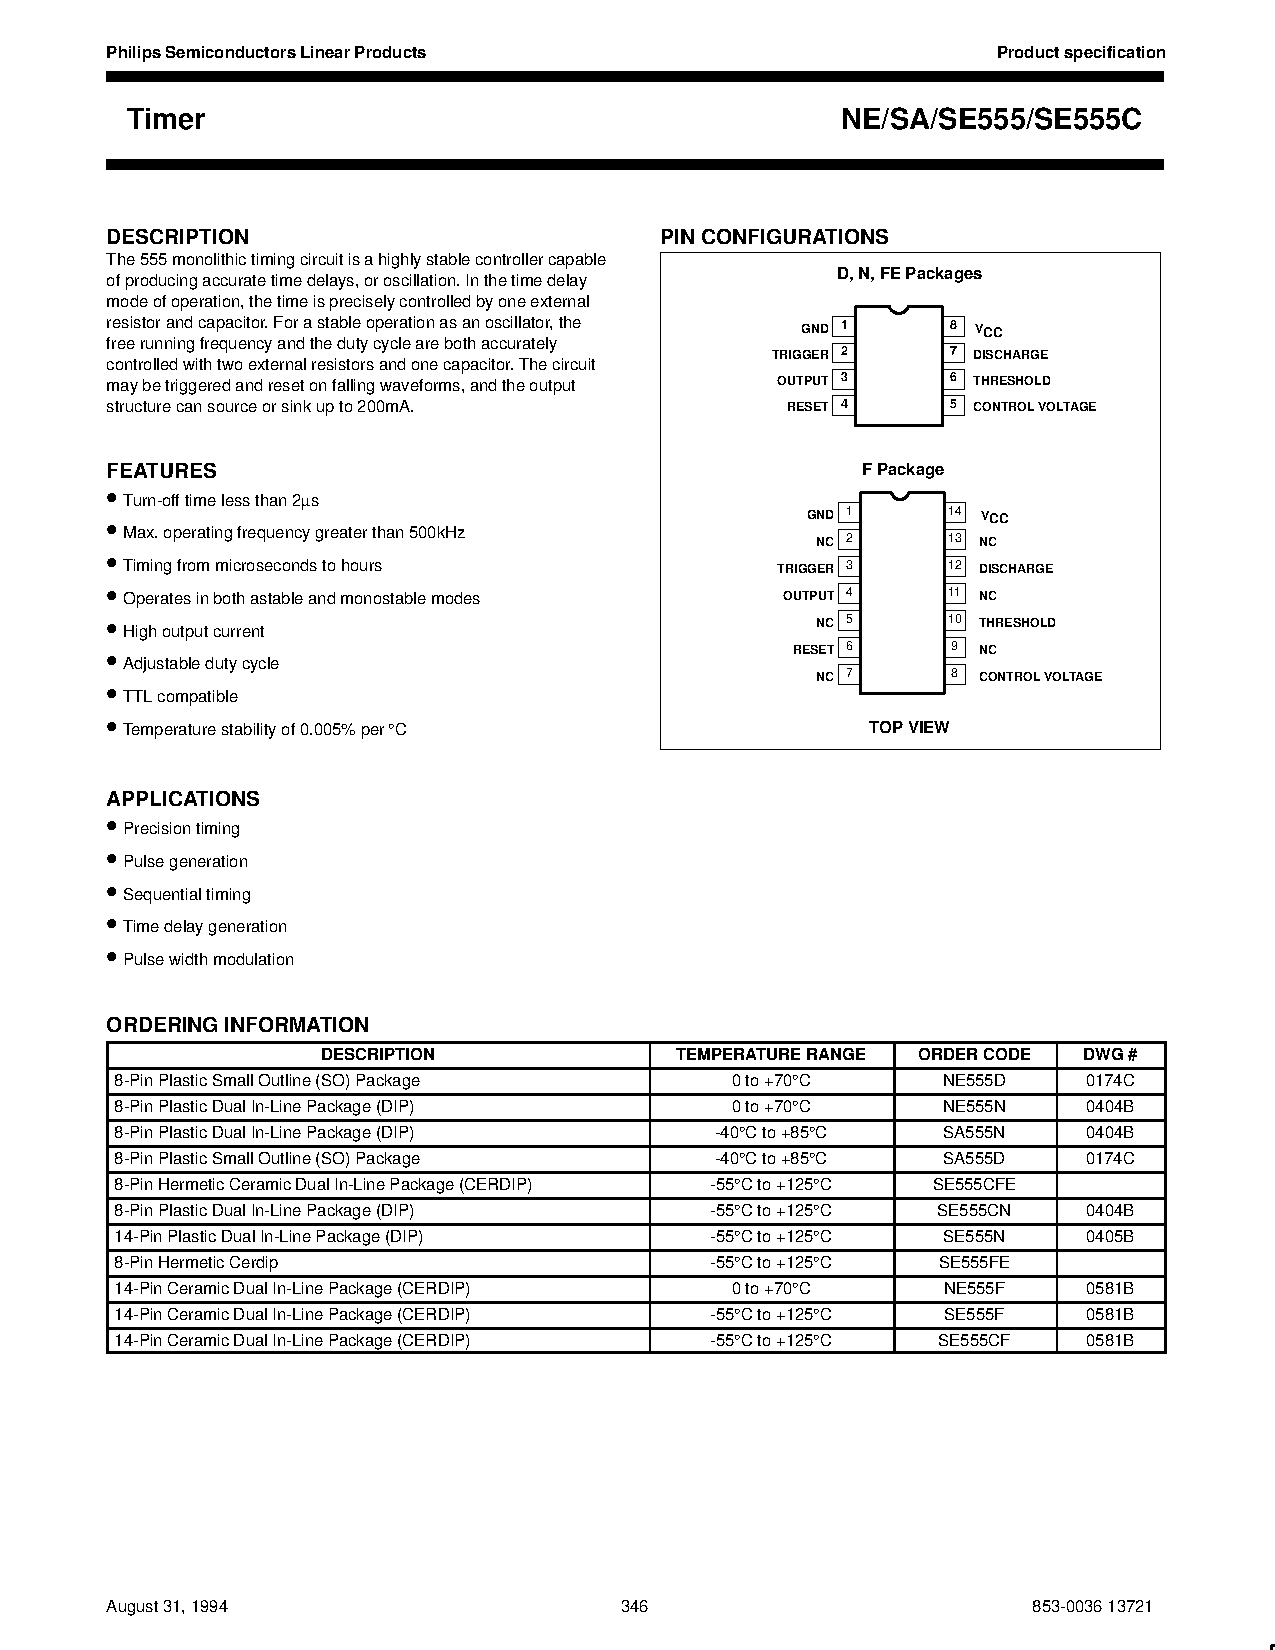
\includepdf[page=2-5,scale=\includepdfscale,pagecommand={ }]{555.pdf}

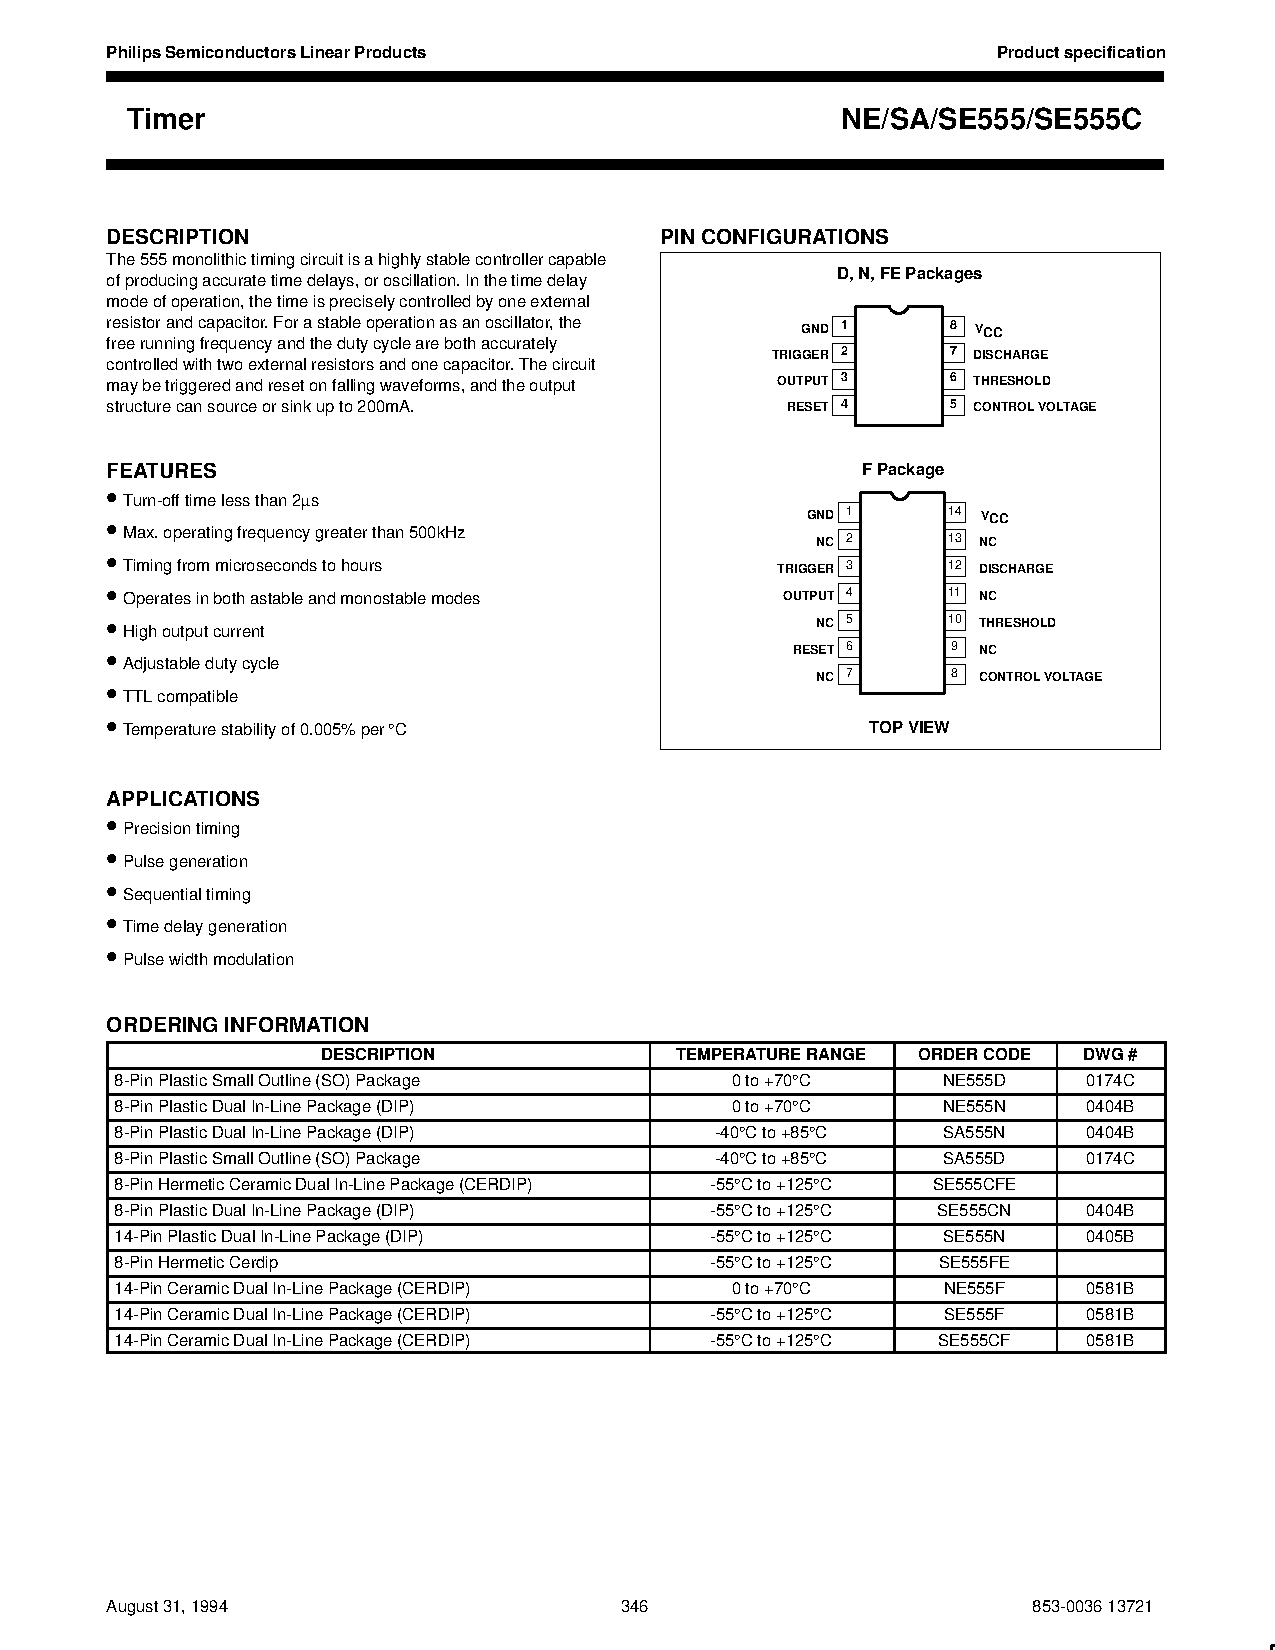
\includepdf[page=6,scale=\includepdfscale,pagecommand={\subsubsection{Typical 555 Application}\hypertarget{555}{}}]{555.pdf}

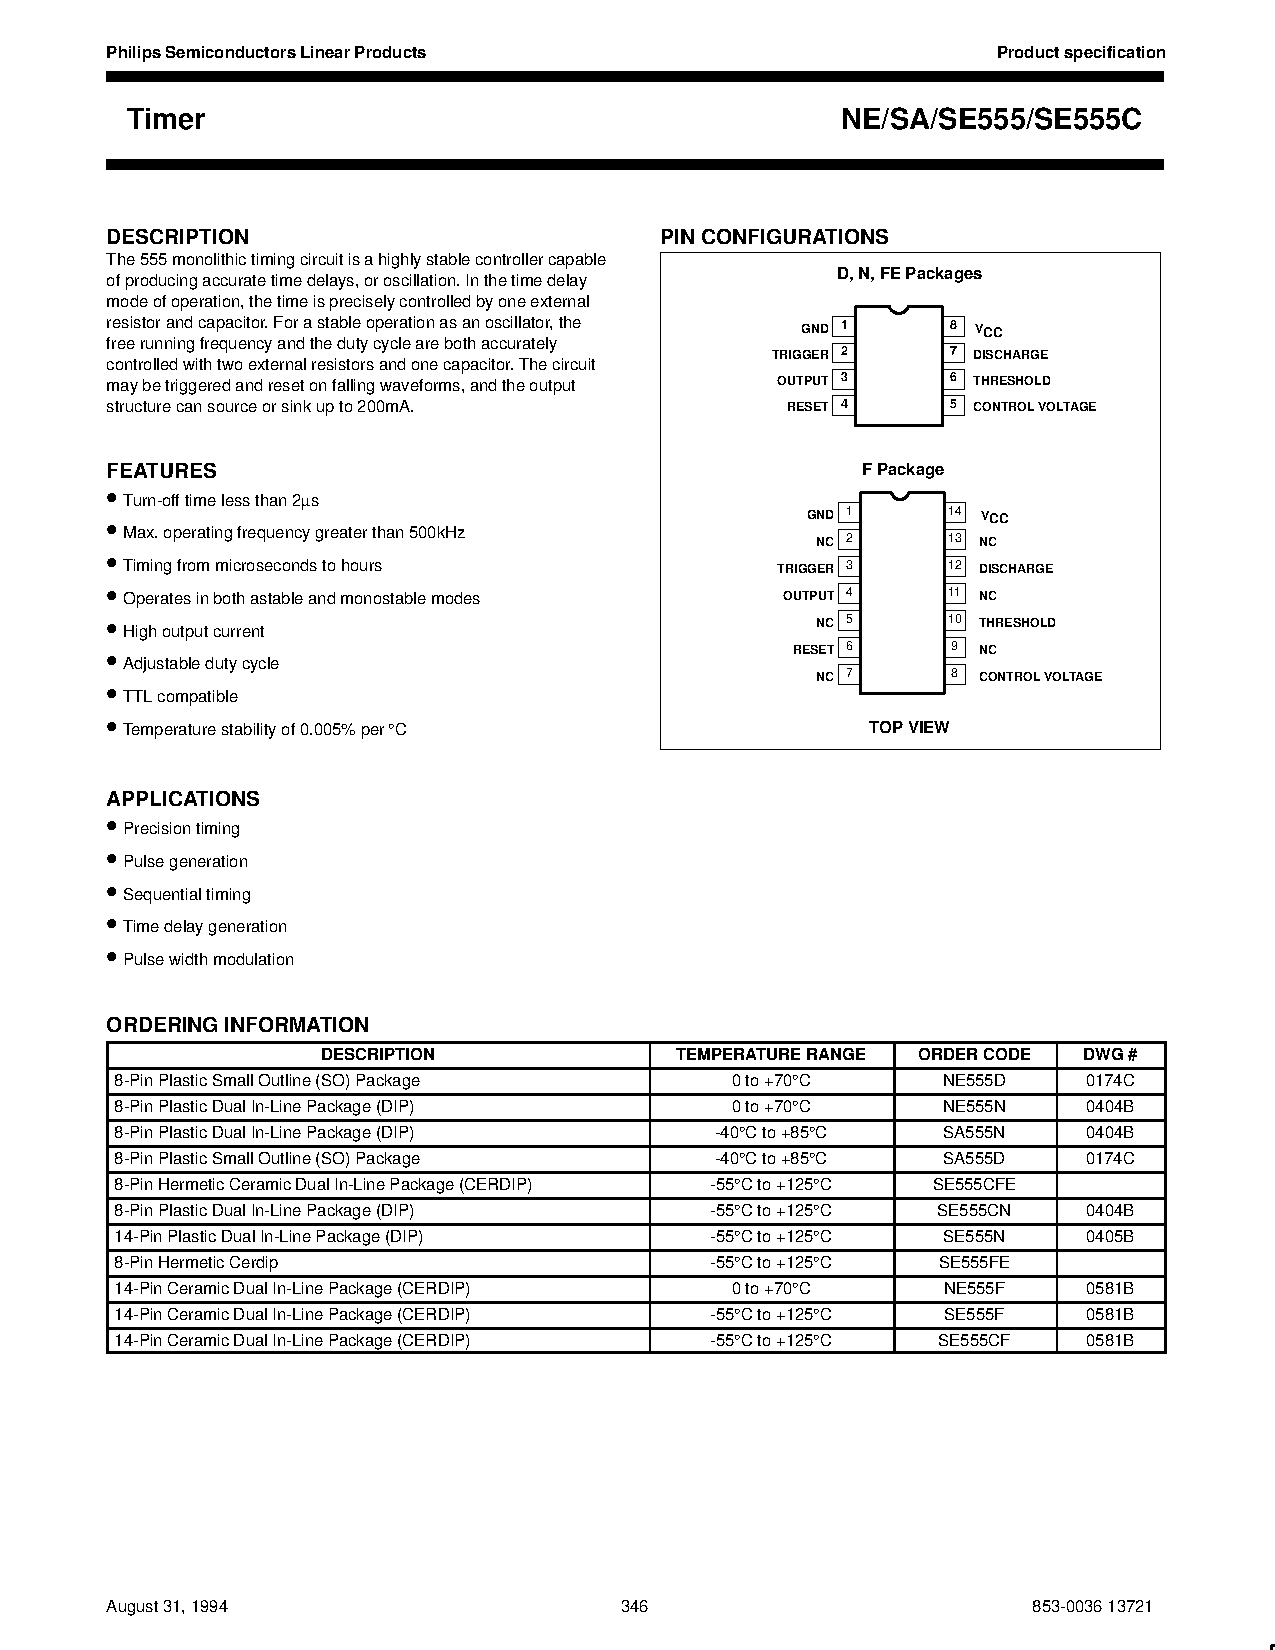
\includepdf[page=7,scale=\includepdfscale,pagecommand={ }]{555.pdf}

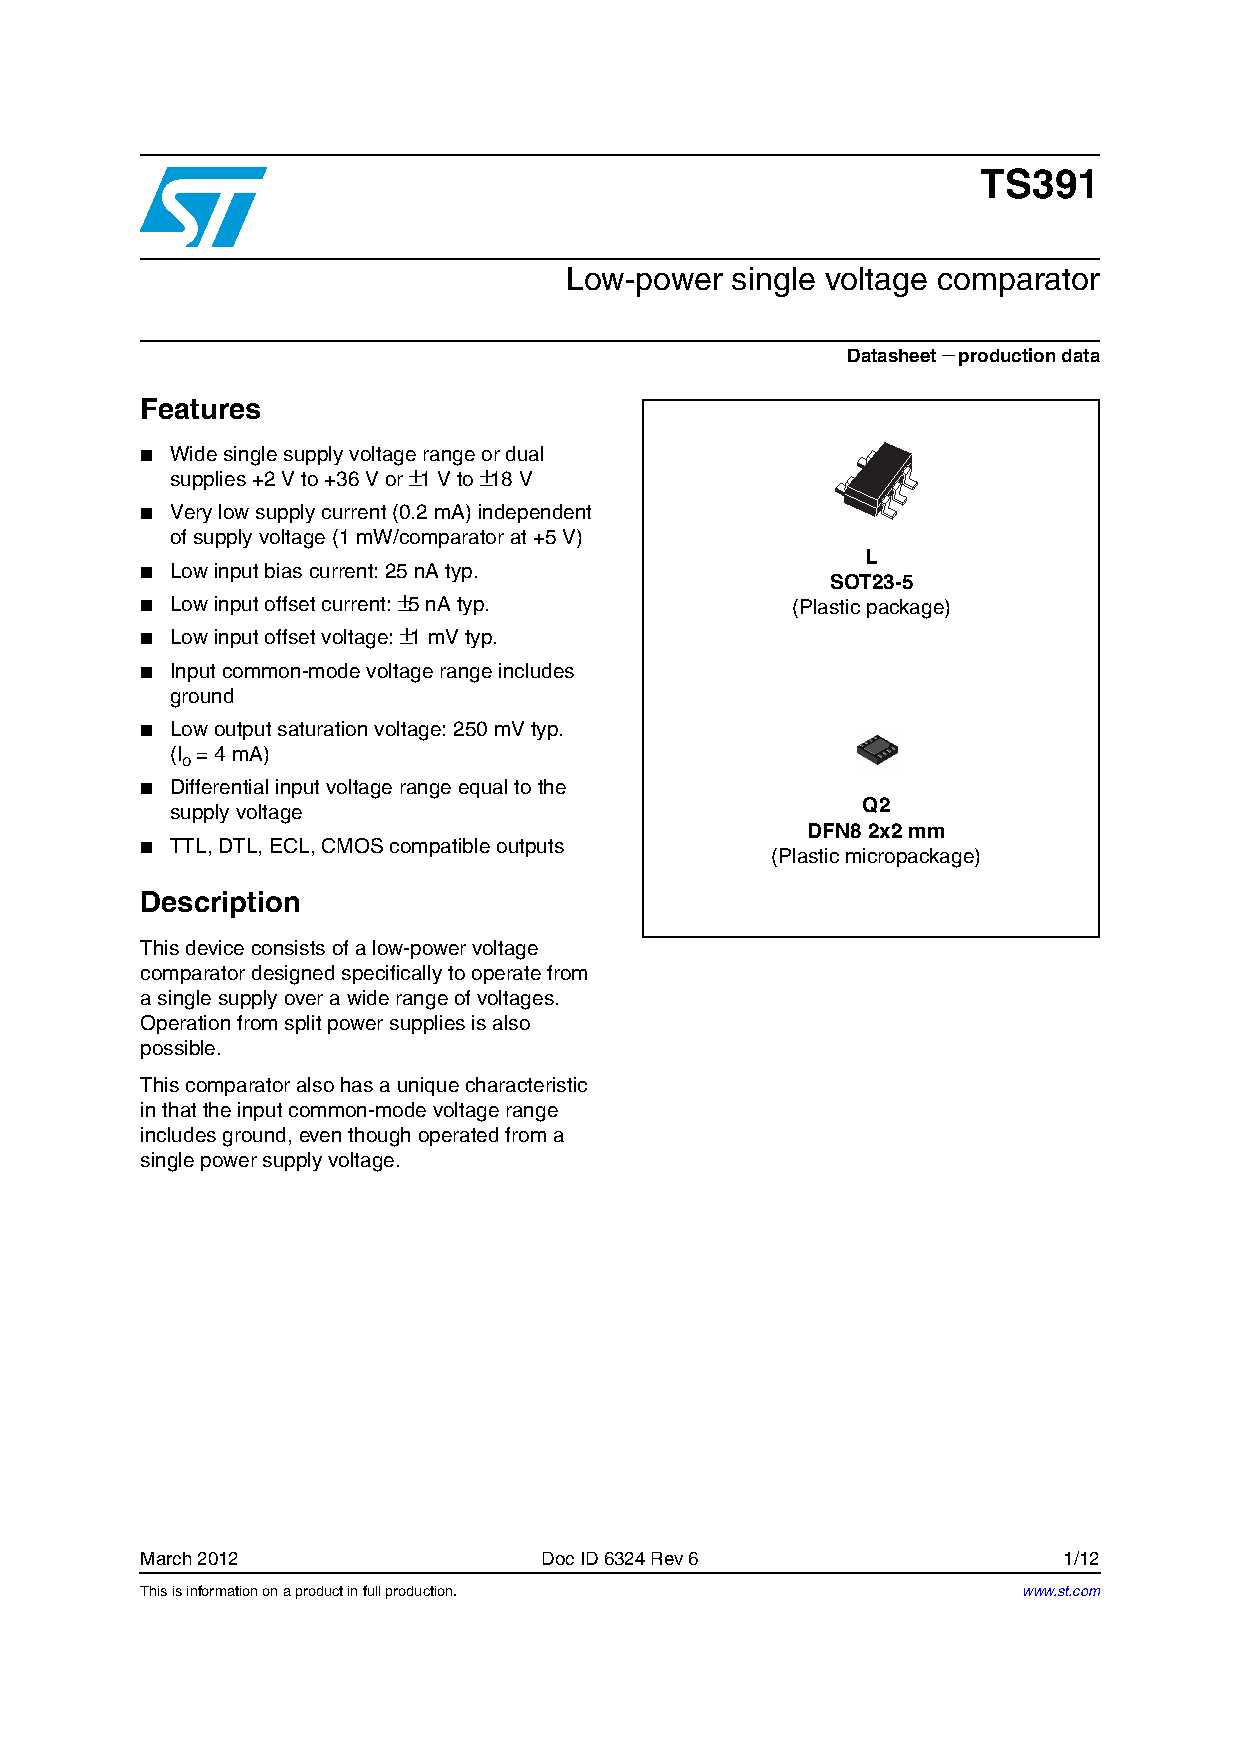
\includepdf[page=1,scale=\includepdfscale,pagecommand={\subsection{Comparateur TS391 Datasheet}\hypertarget{Comparateur}{}}]{Comparateur.pdf}

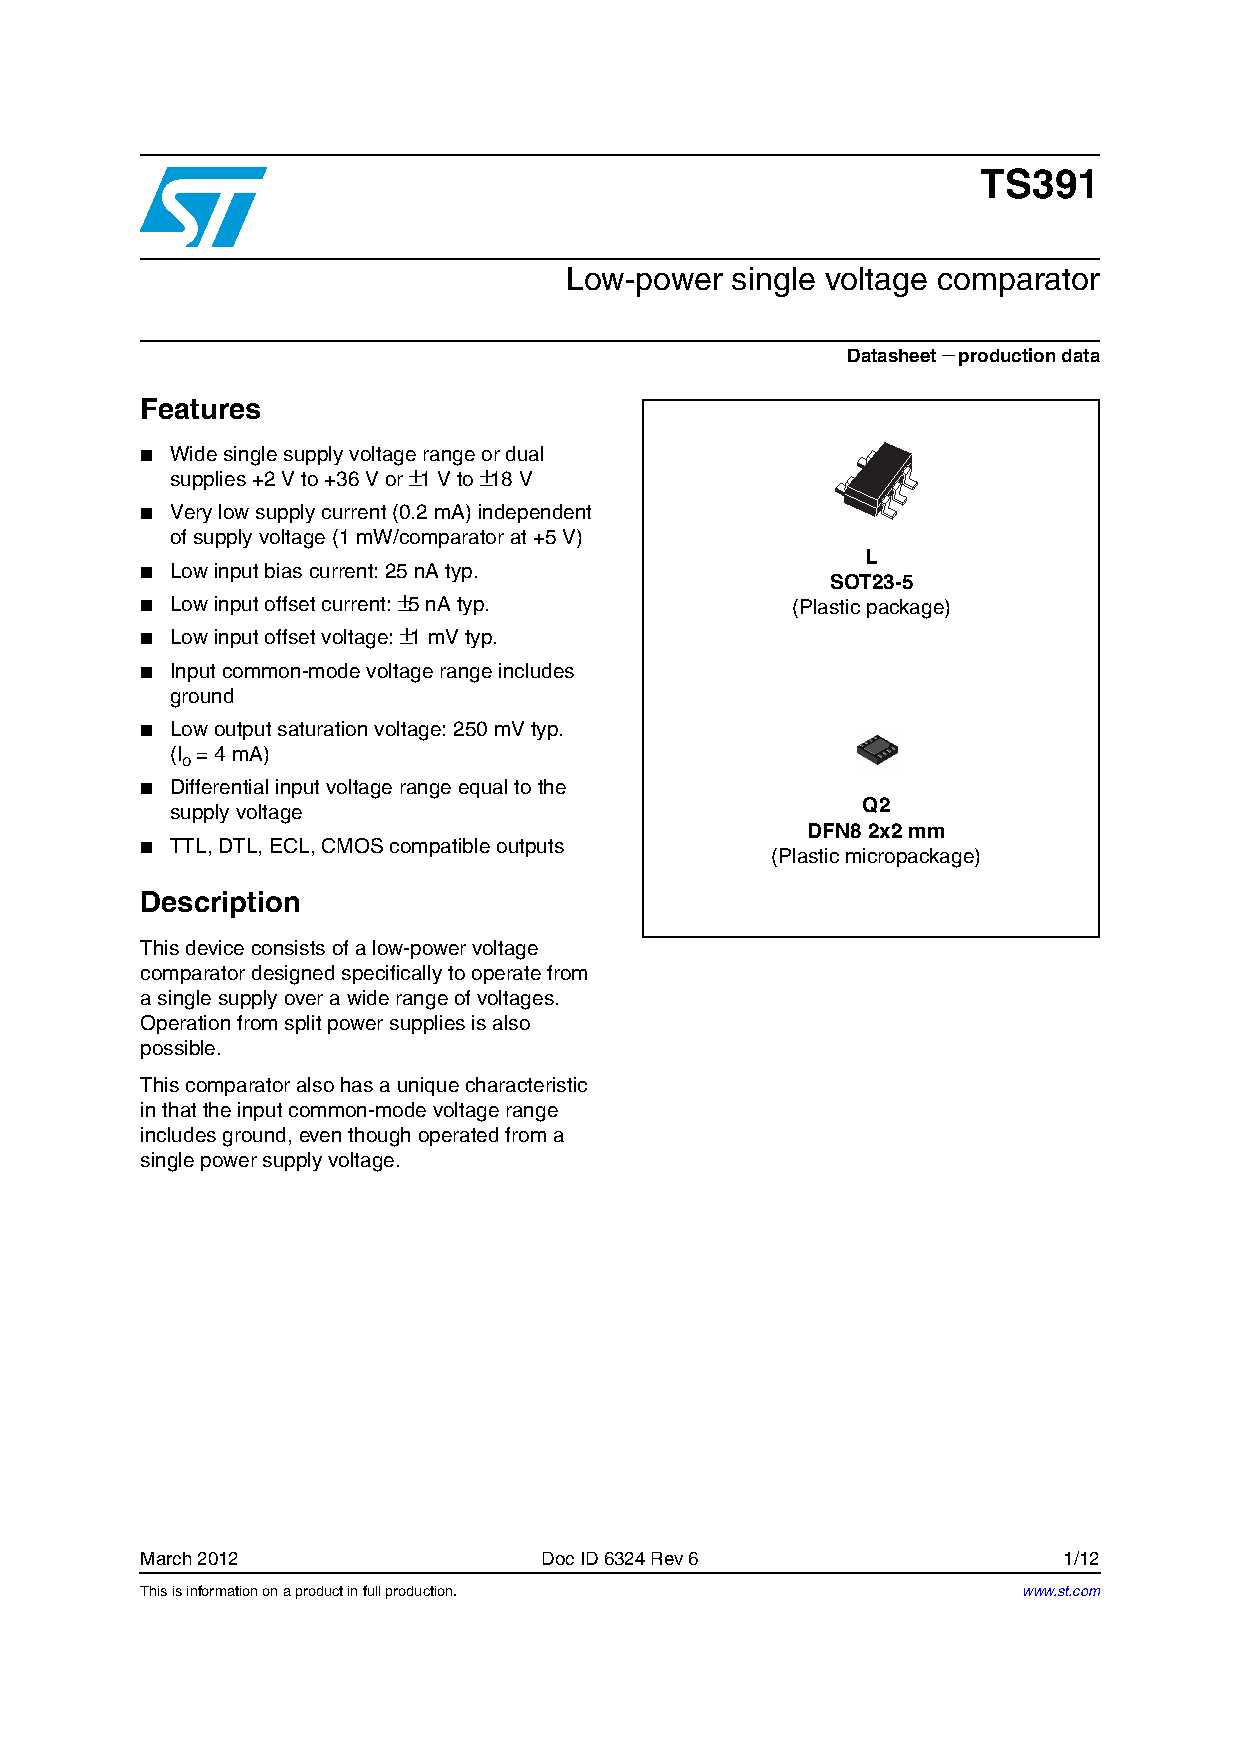
\includepdf[page=2,scale=\includepdfscale,pagecommand={\subsubsection{Schematic Diagram}\hypertarget{AmpliOp}{}}]{Comparateur.pdf}

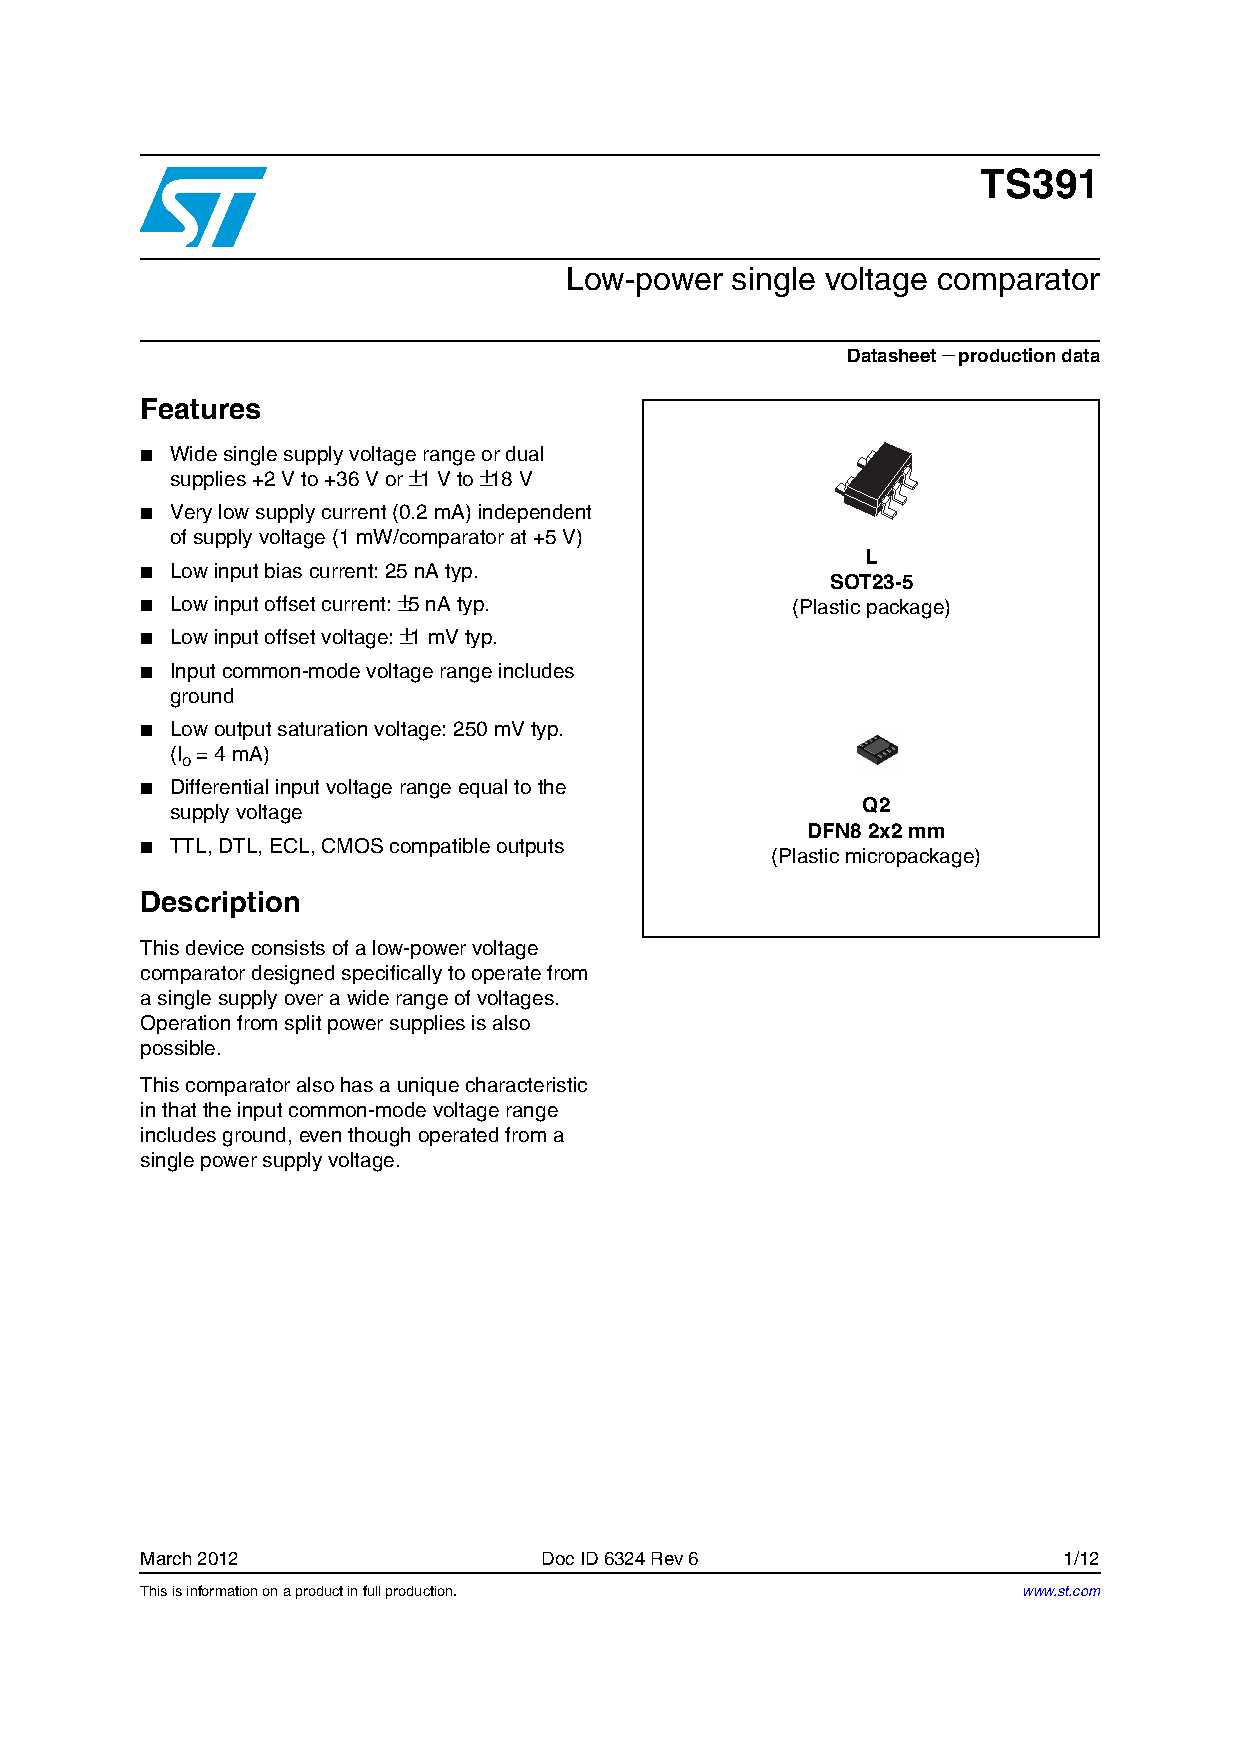
\includepdf[page=3-5,scale=\includepdfscale,pagecommand={ }]{Comparateur.pdf}
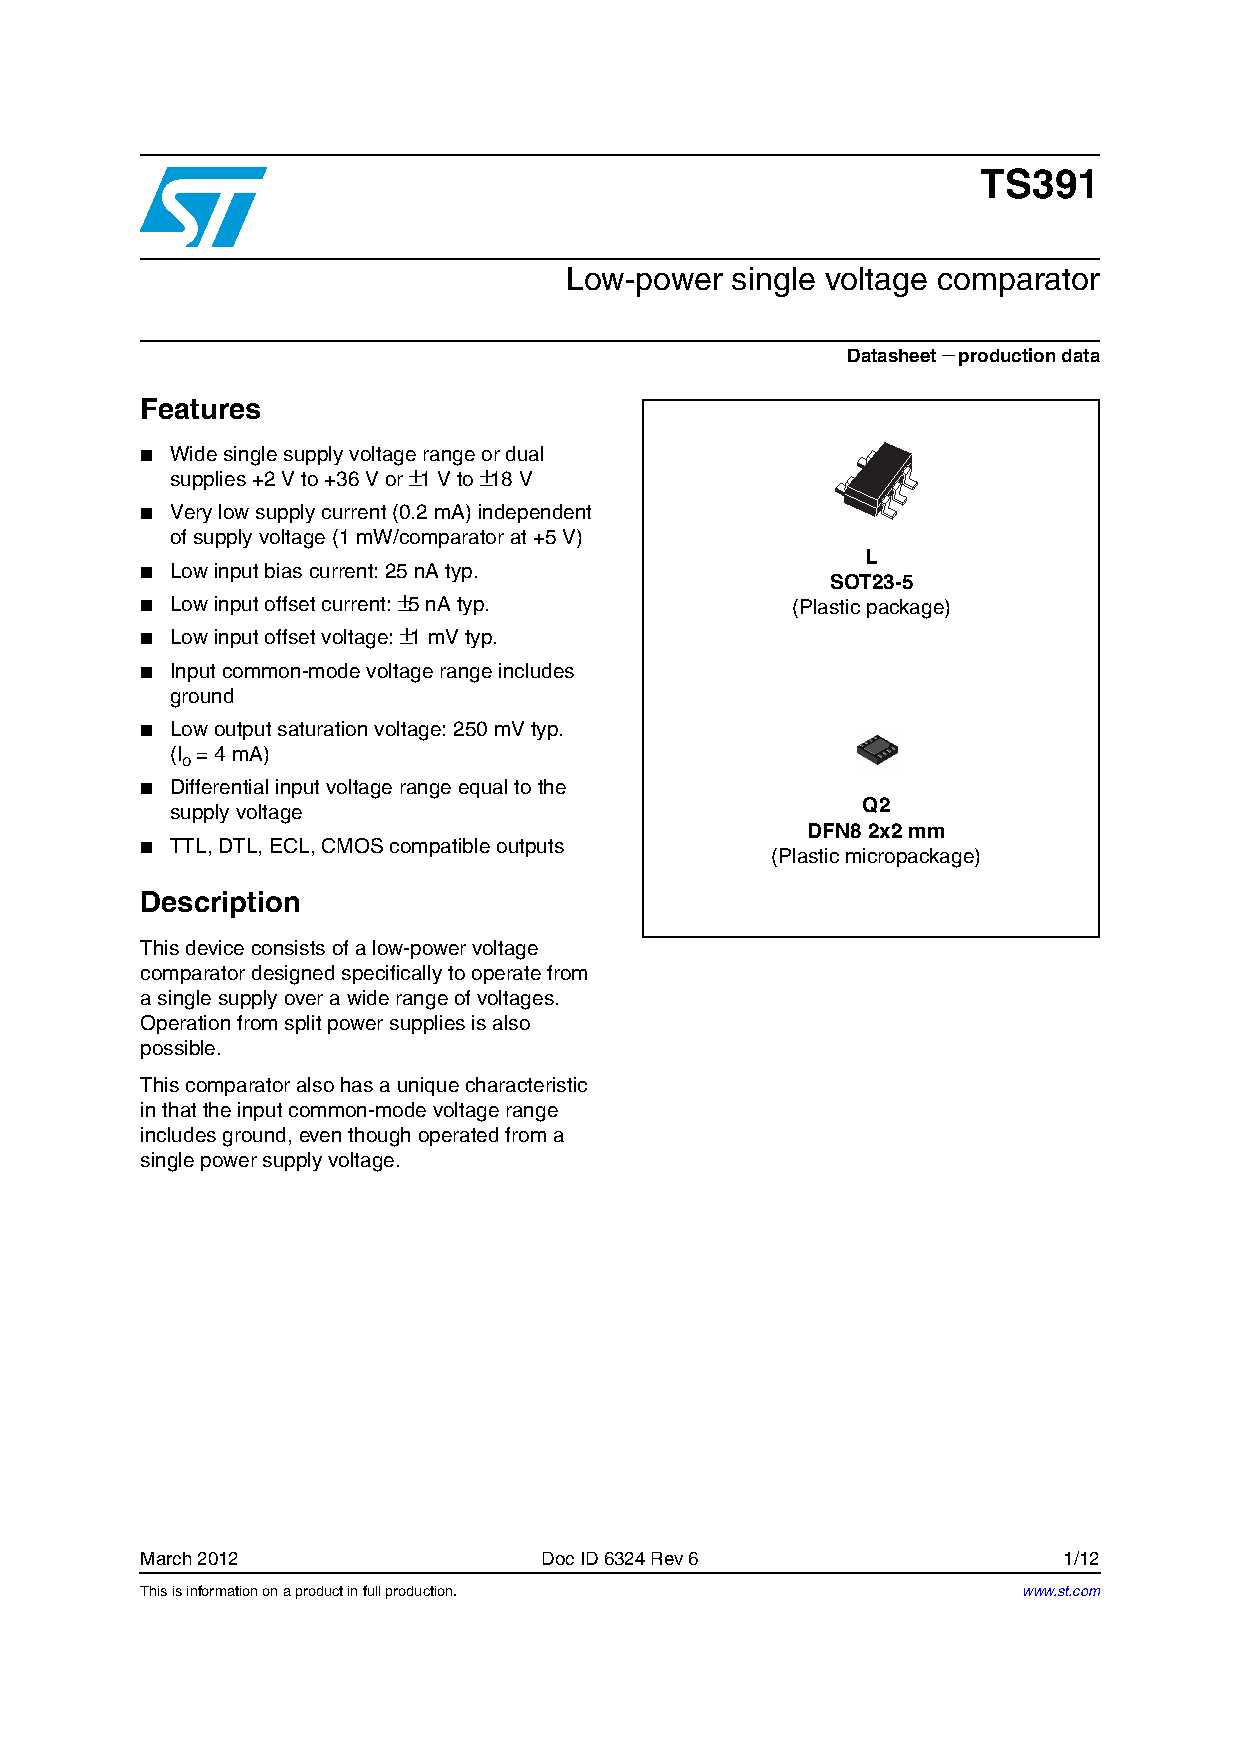
\includepdf[page=9-10,scale=\includepdfscale,pagecommand={ }]{Comparateur.pdf}

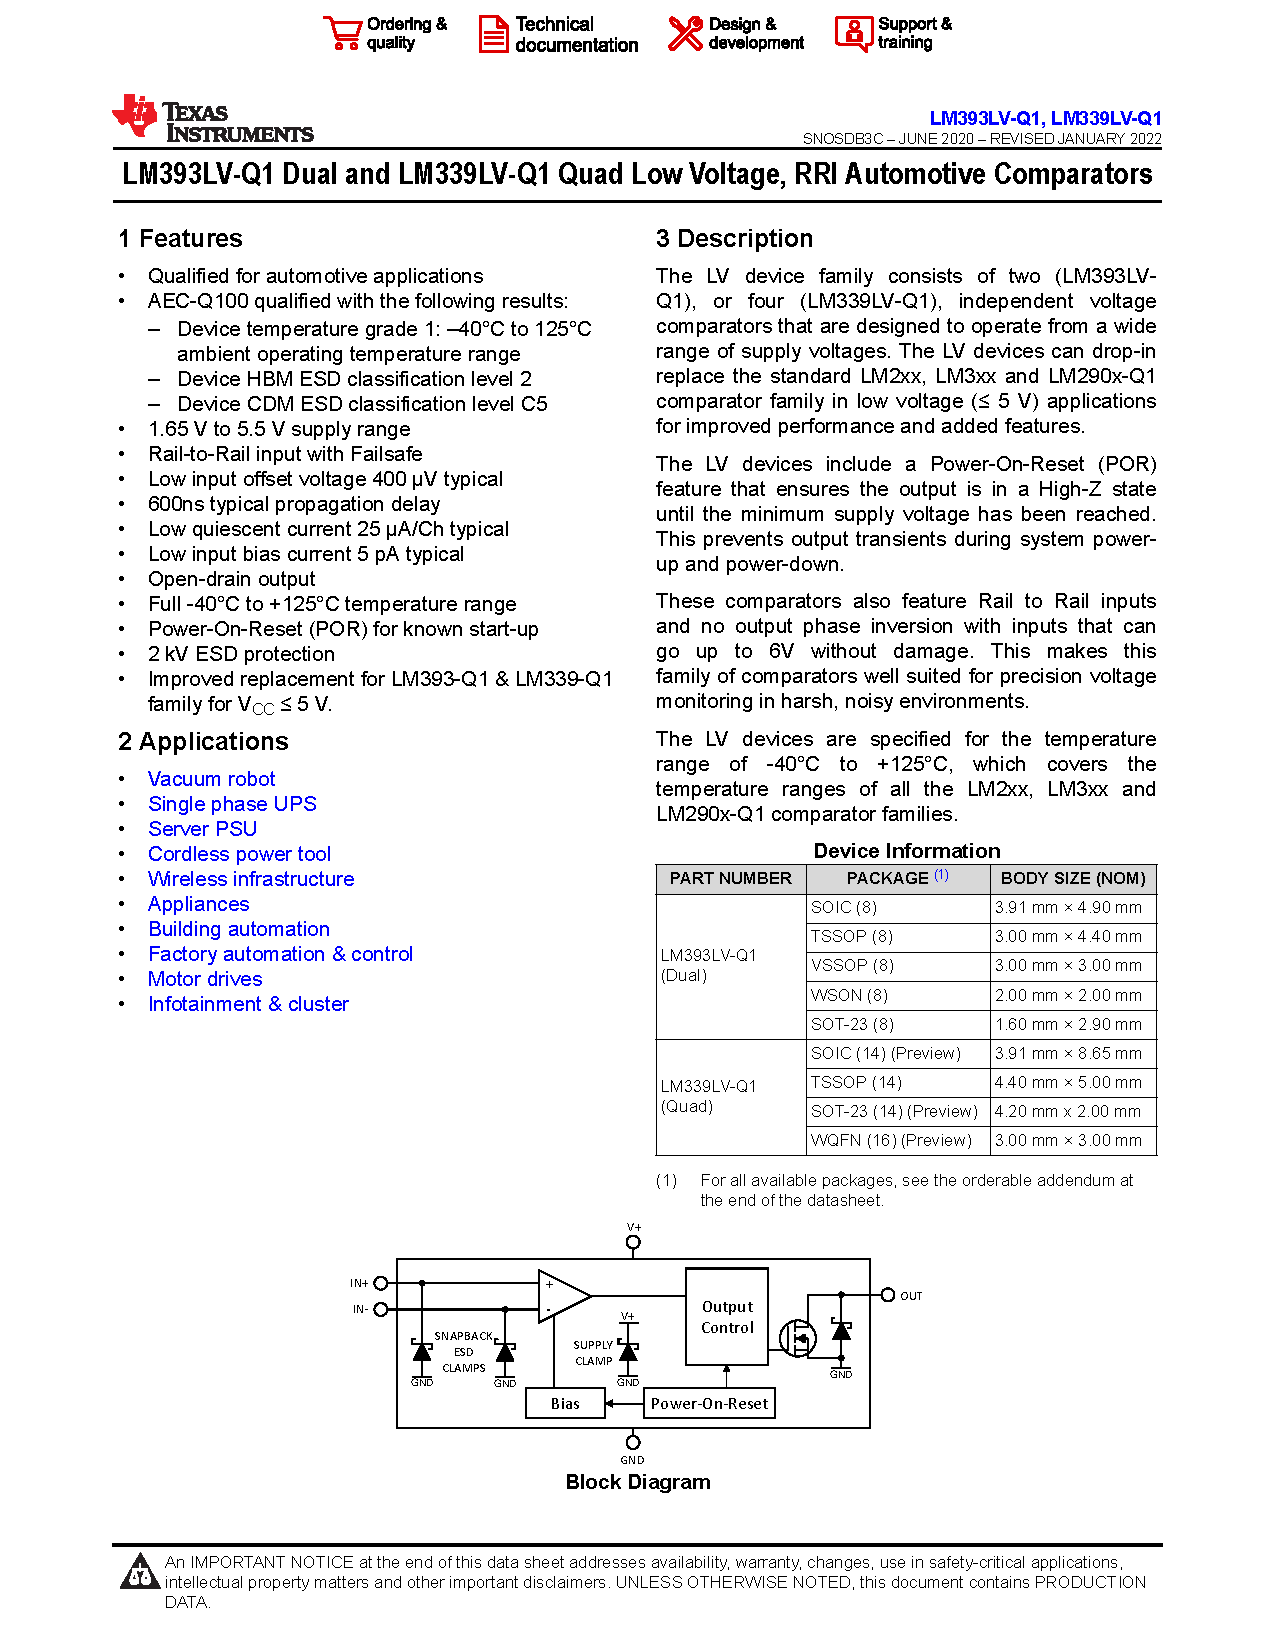
\includepdf[page=1,scale=\includepdfscale,pagecommand={\subsection{Comparateur double LM393LV-Q1 Datasheet}\hypertarget{ComparateurDouble}{}}]{Comparateur double_1.pdf}
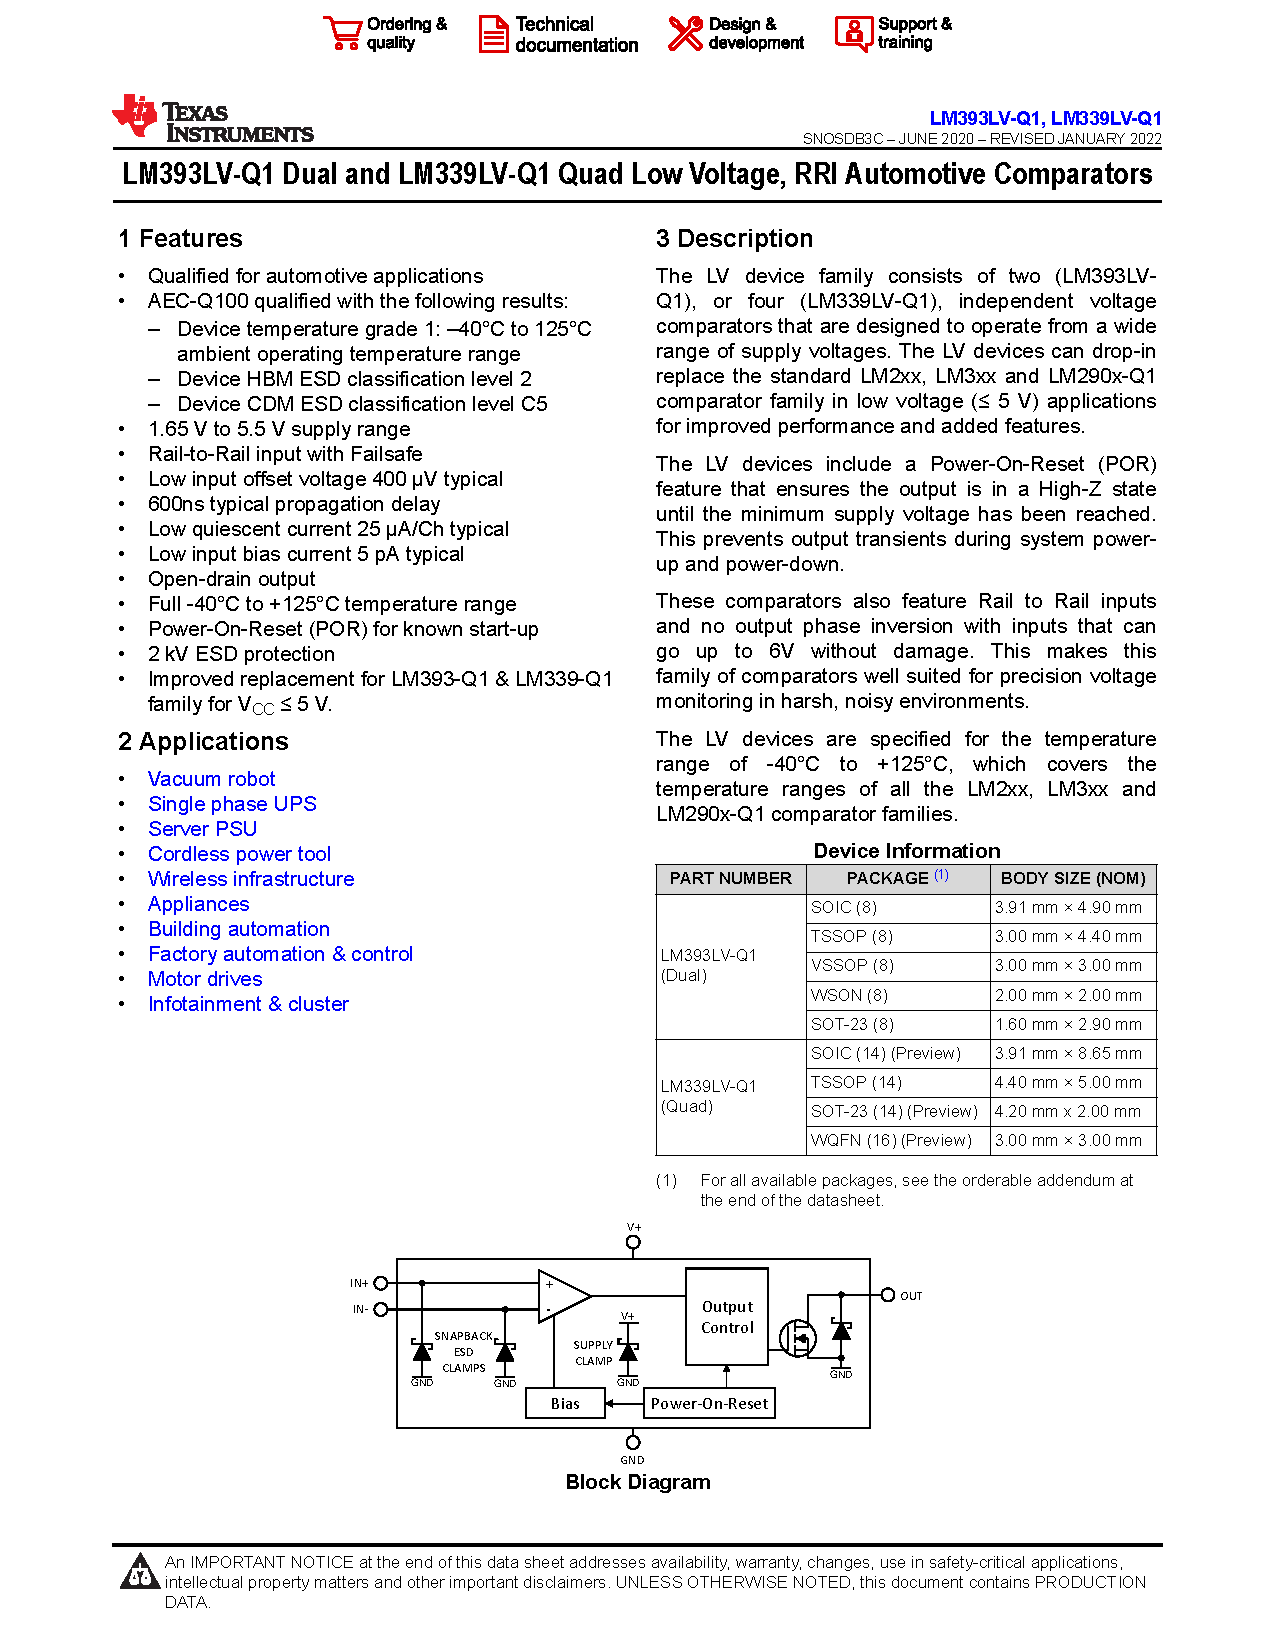
\includepdf[page=2-3,scale=\includepdfscale,pagecommand={}]{Comparateur double_1.pdf}
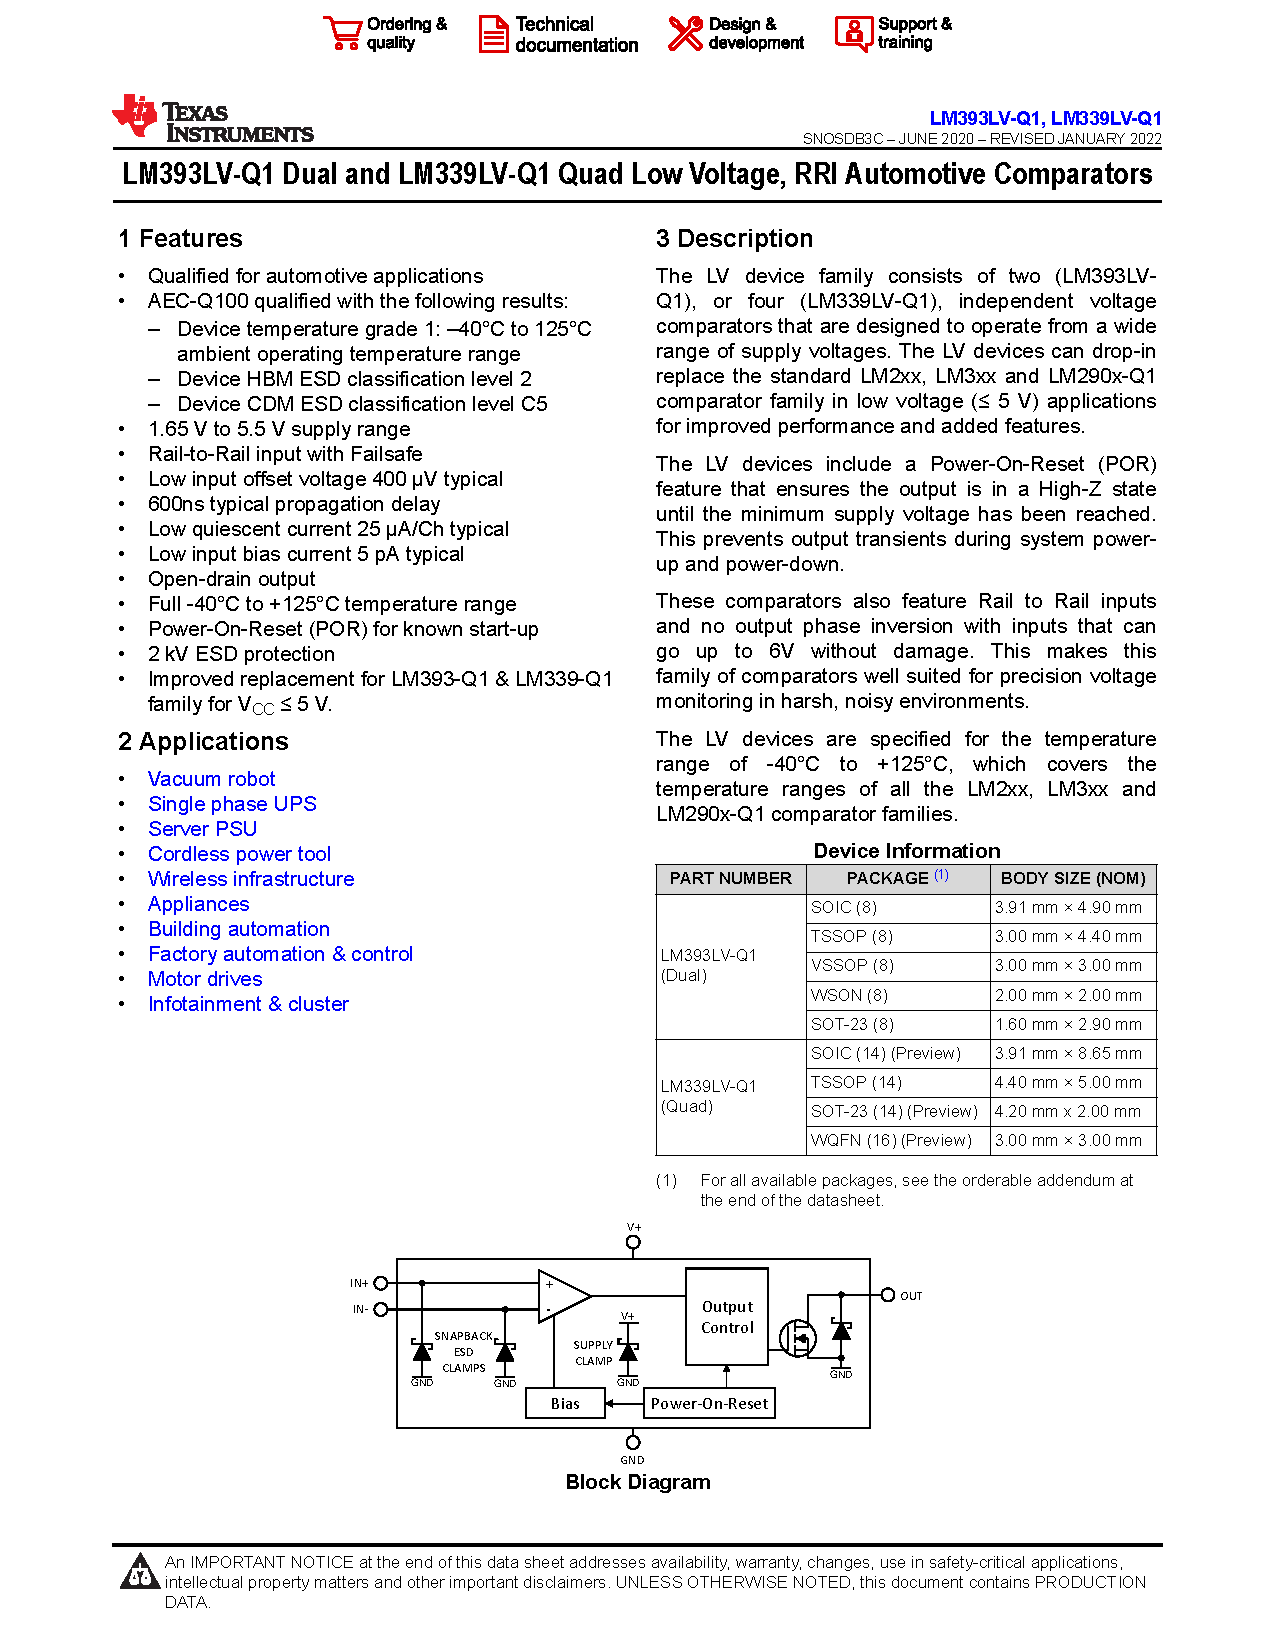
\includepdf[page=5-30,scale=\includepdfscale,pagecommand={}]{Comparateur double_1.pdf}

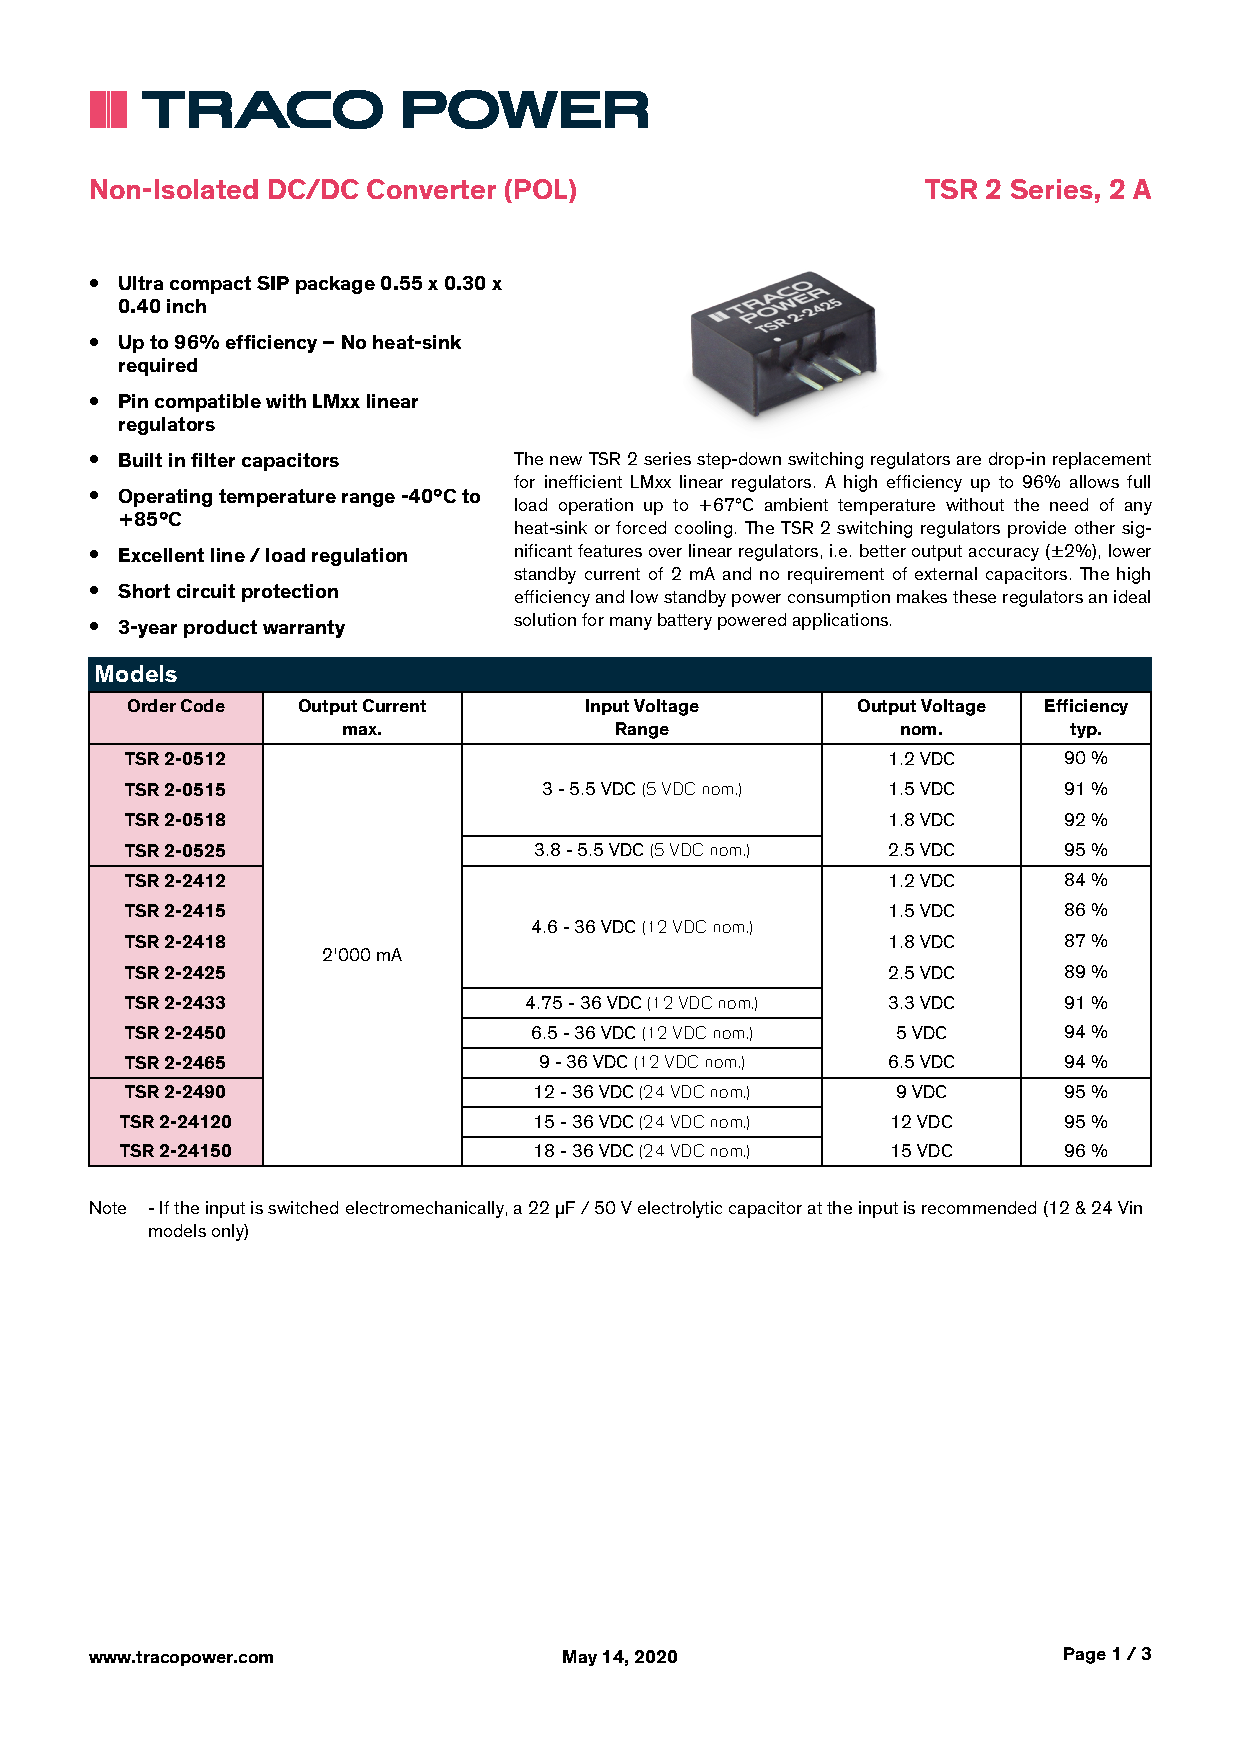
\includepdf[page=1,scale=\includepdfscale,pagecommand={\subsection{Alimentation Isolé Datasheet}\hypertarget{AlimIsol}{}}]{Regulateur de tension.pdf}
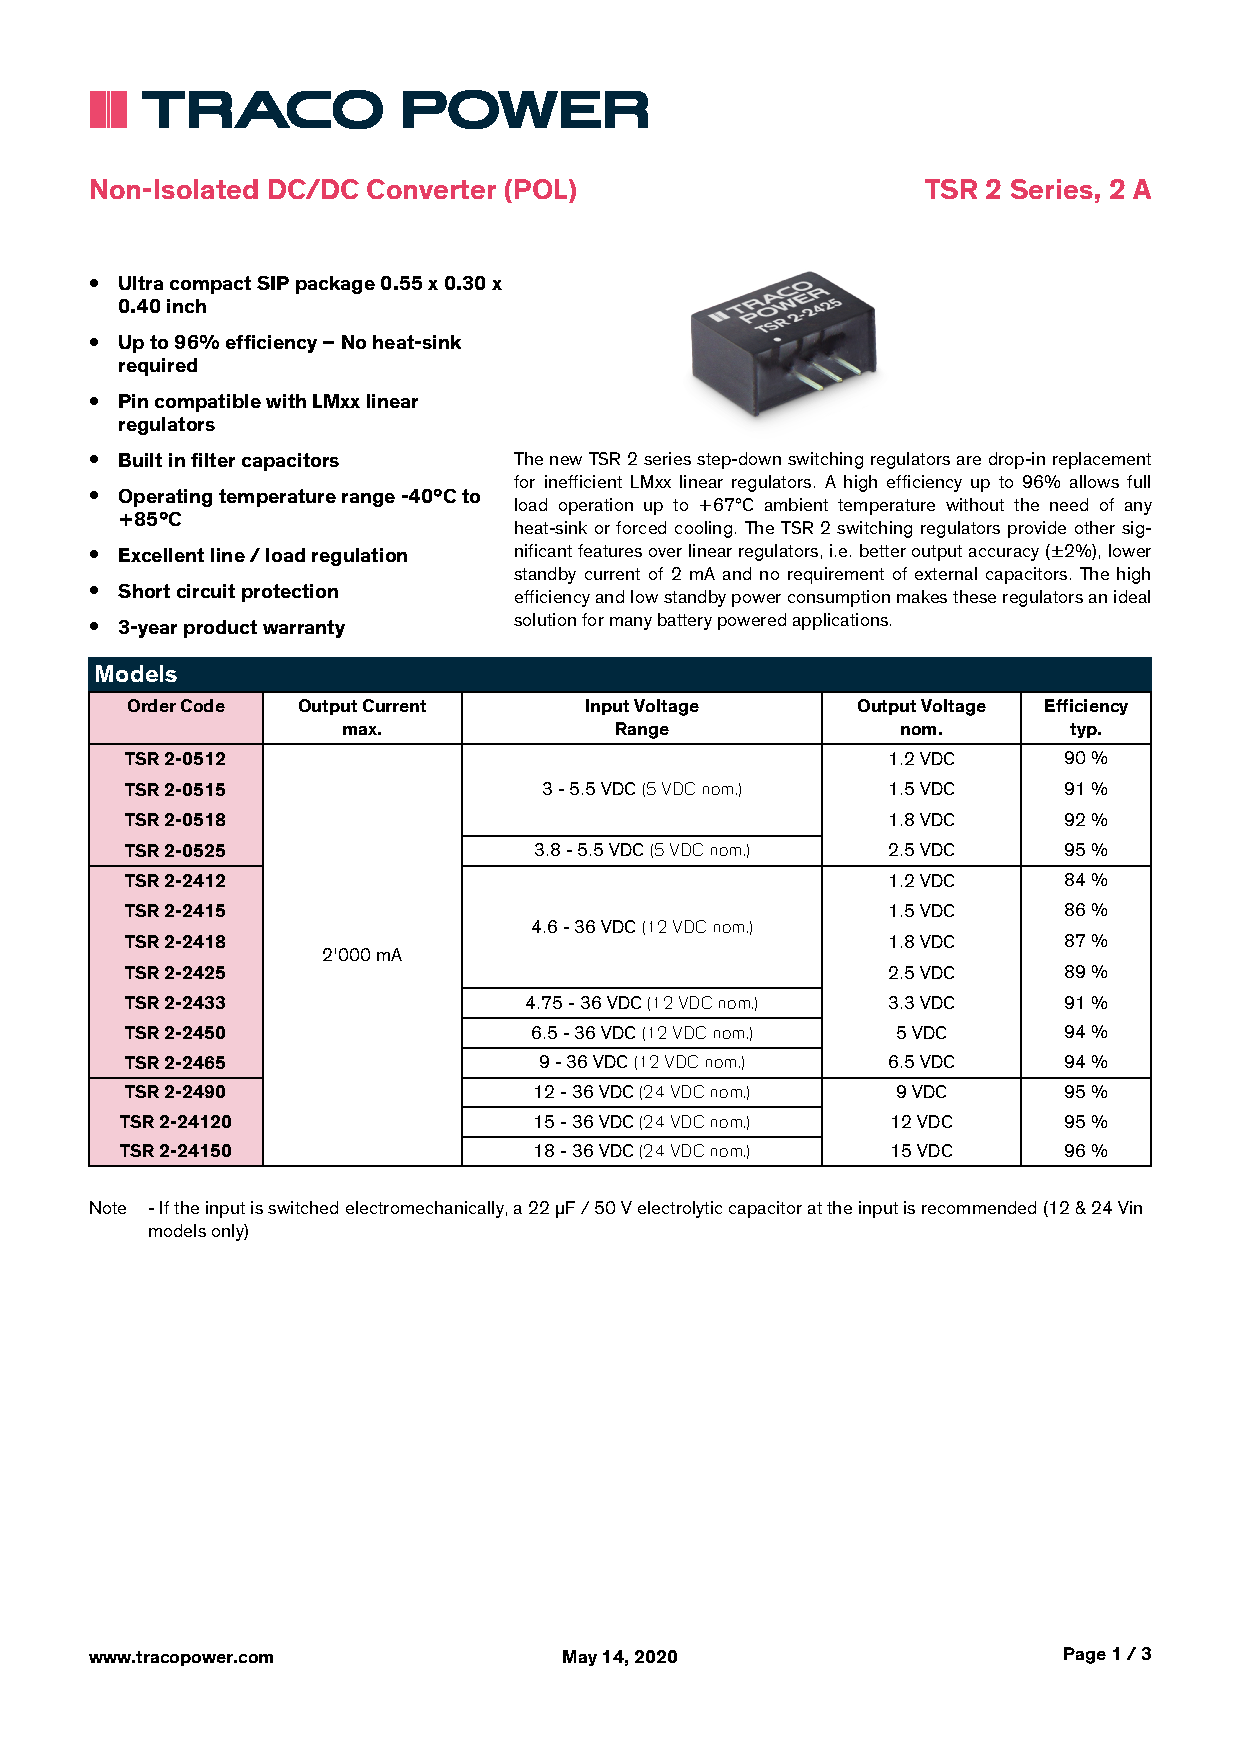
\includepdf[page=2-3,scale=\includepdfscale,pagecommand={}]{Regulateur de tension.pdf}

\includepdf[page=1,scale=\includepdfscale,pagecommand={\subsection{Alimentation Datasheet}\hypertarget{Alim}{}}]{Regulateur de tension isolé.pdf}
\includepdf[page=2-6,scale=\includepdfscale,pagecommand={}]{Regulateur de tension isolé.pdf}


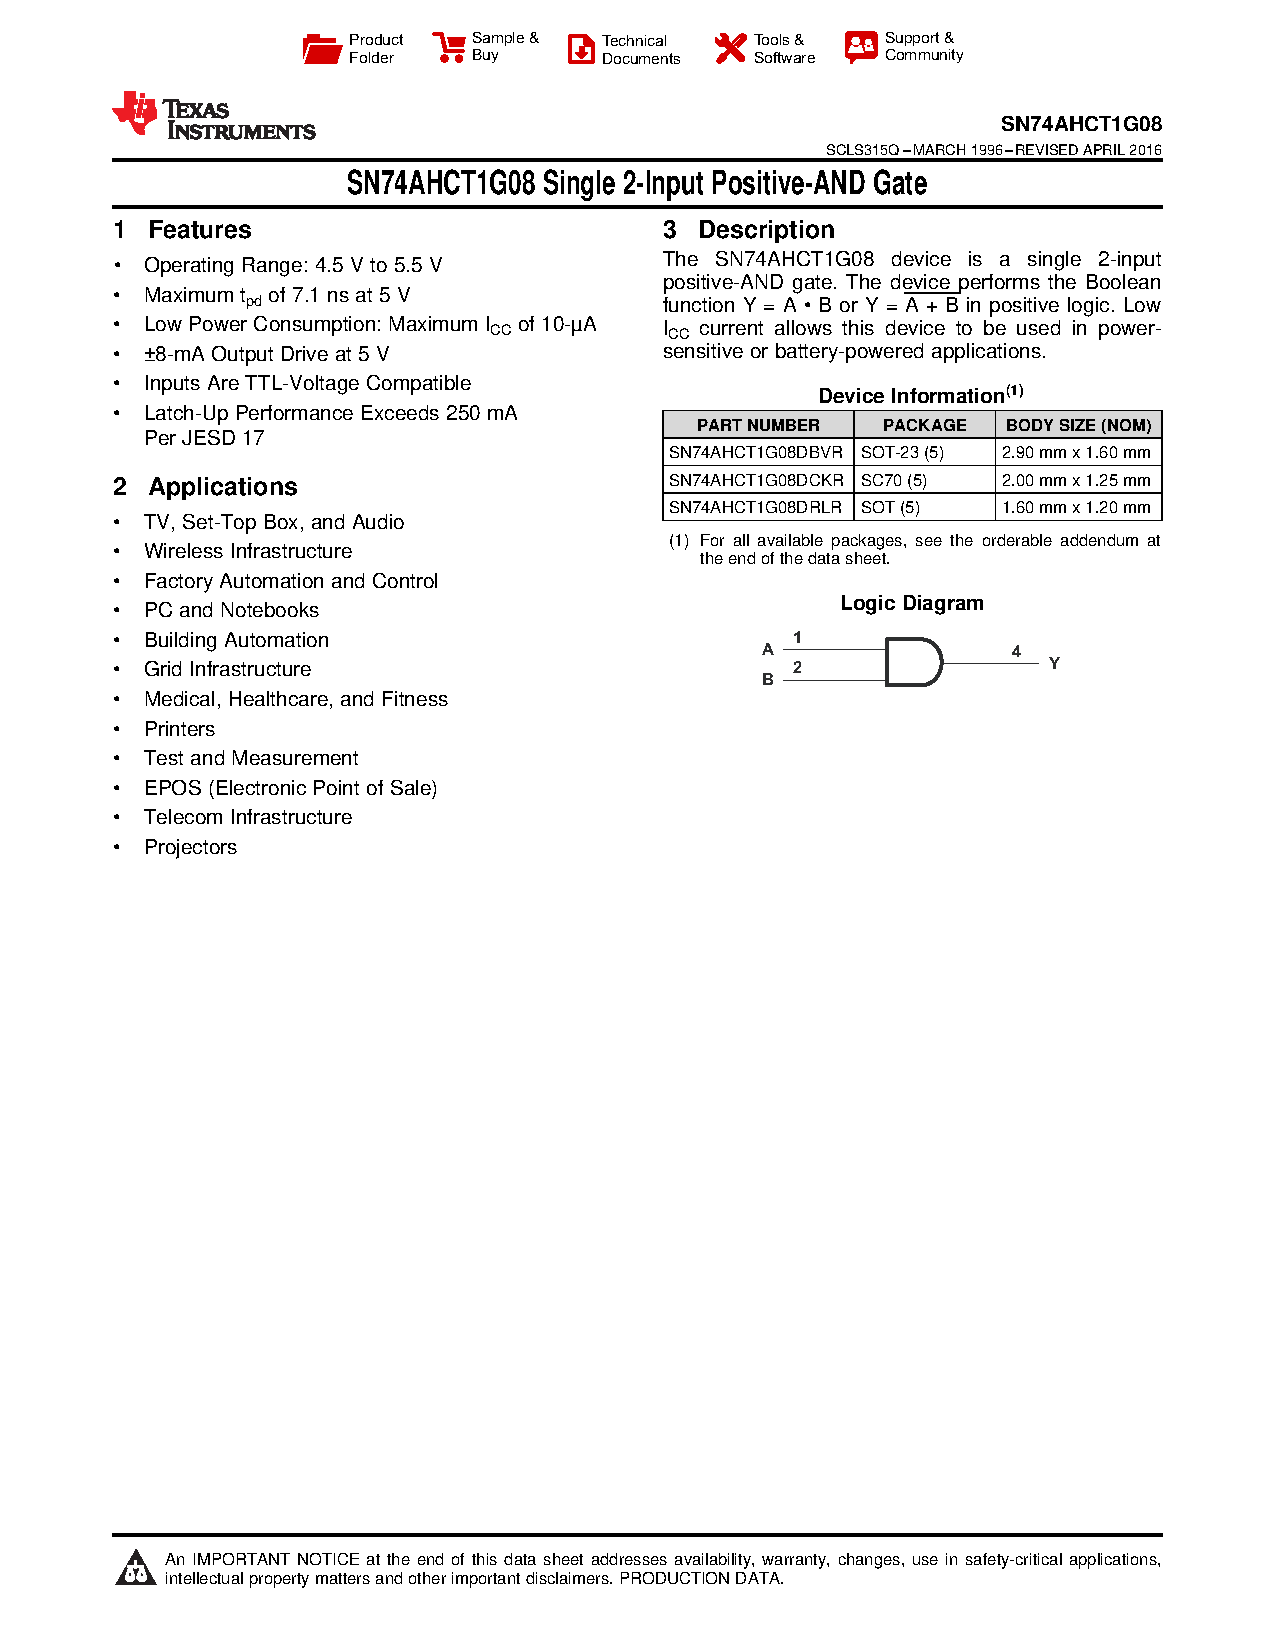
\includepdf[page=1,scale=0.78,pagecommand={\subsection{Porte Logique}\subsubsection{Porte And Datasheet}\hypertarget{And}{}}]{Gate AND.pdf}
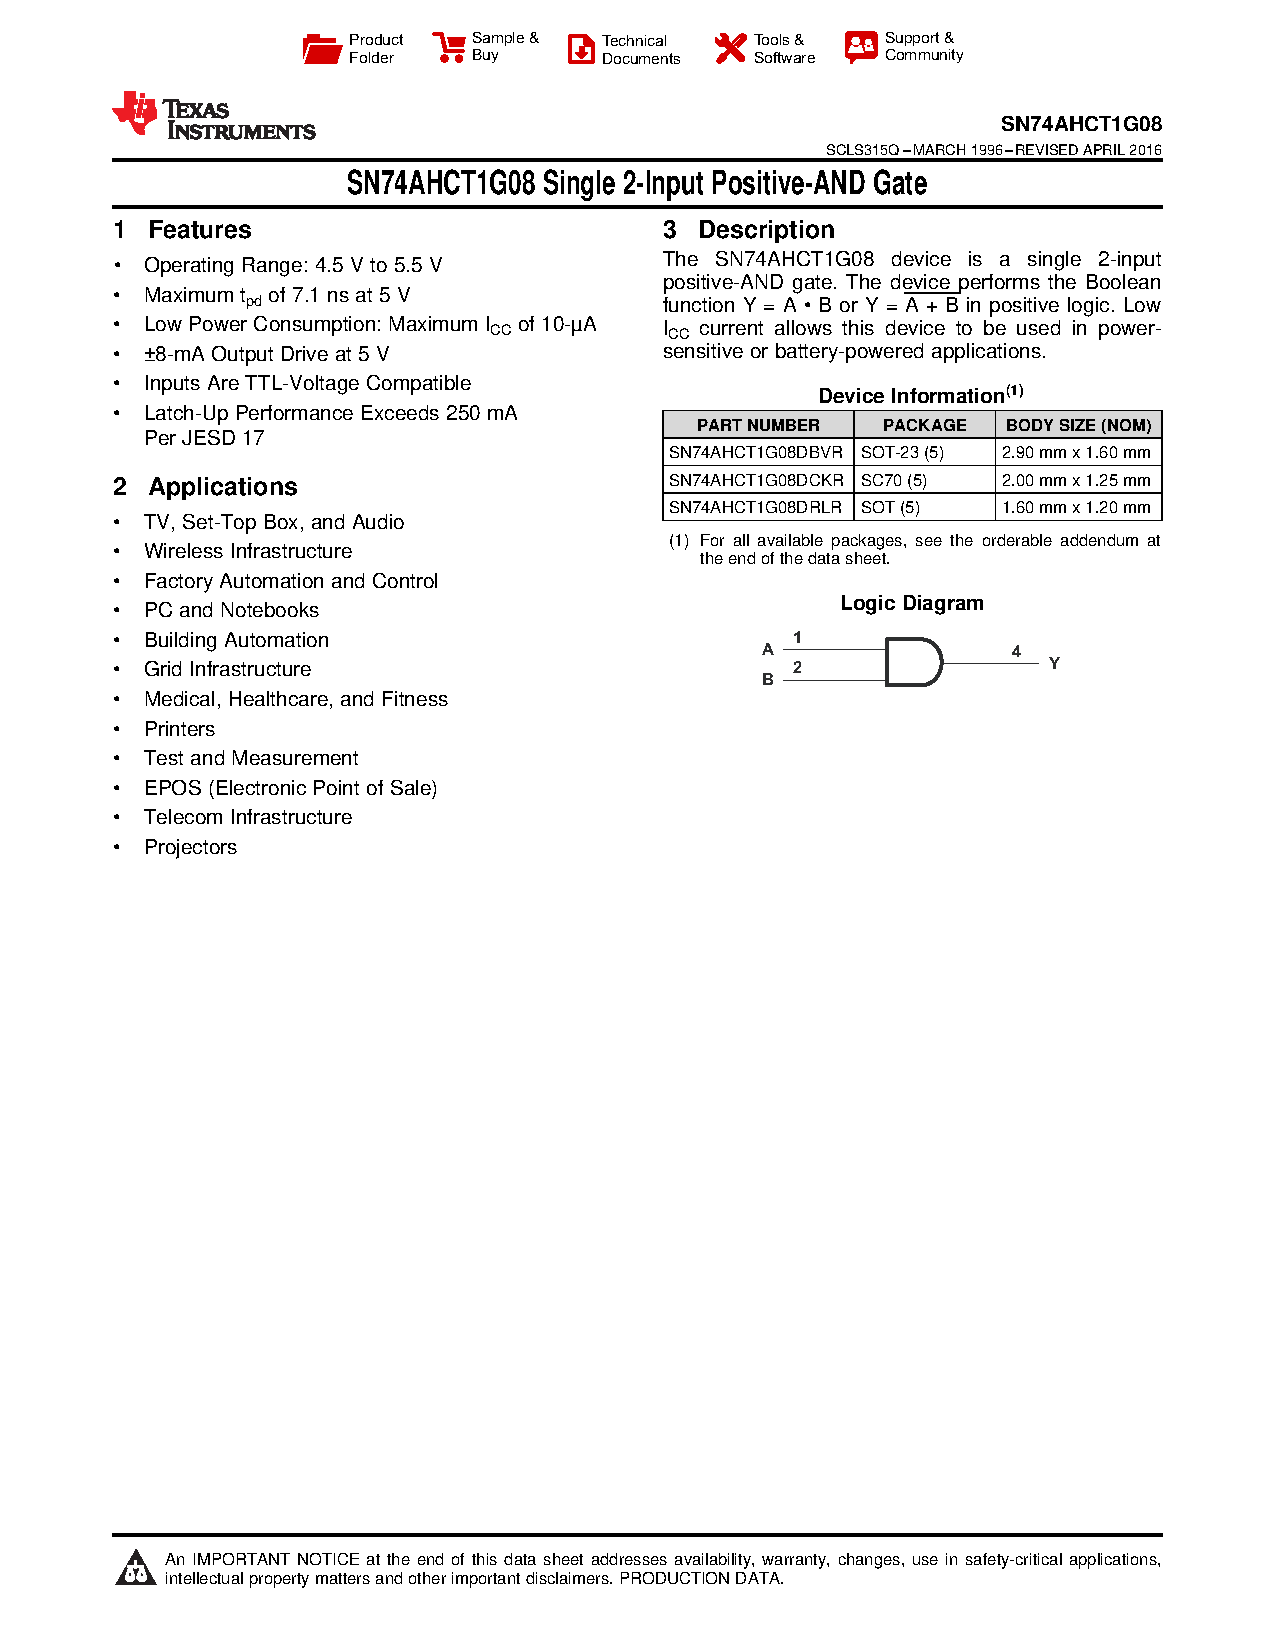
\includepdf[page=2-10,scale=\includepdfscale,pagecommand={}]{Gate AND.pdf}

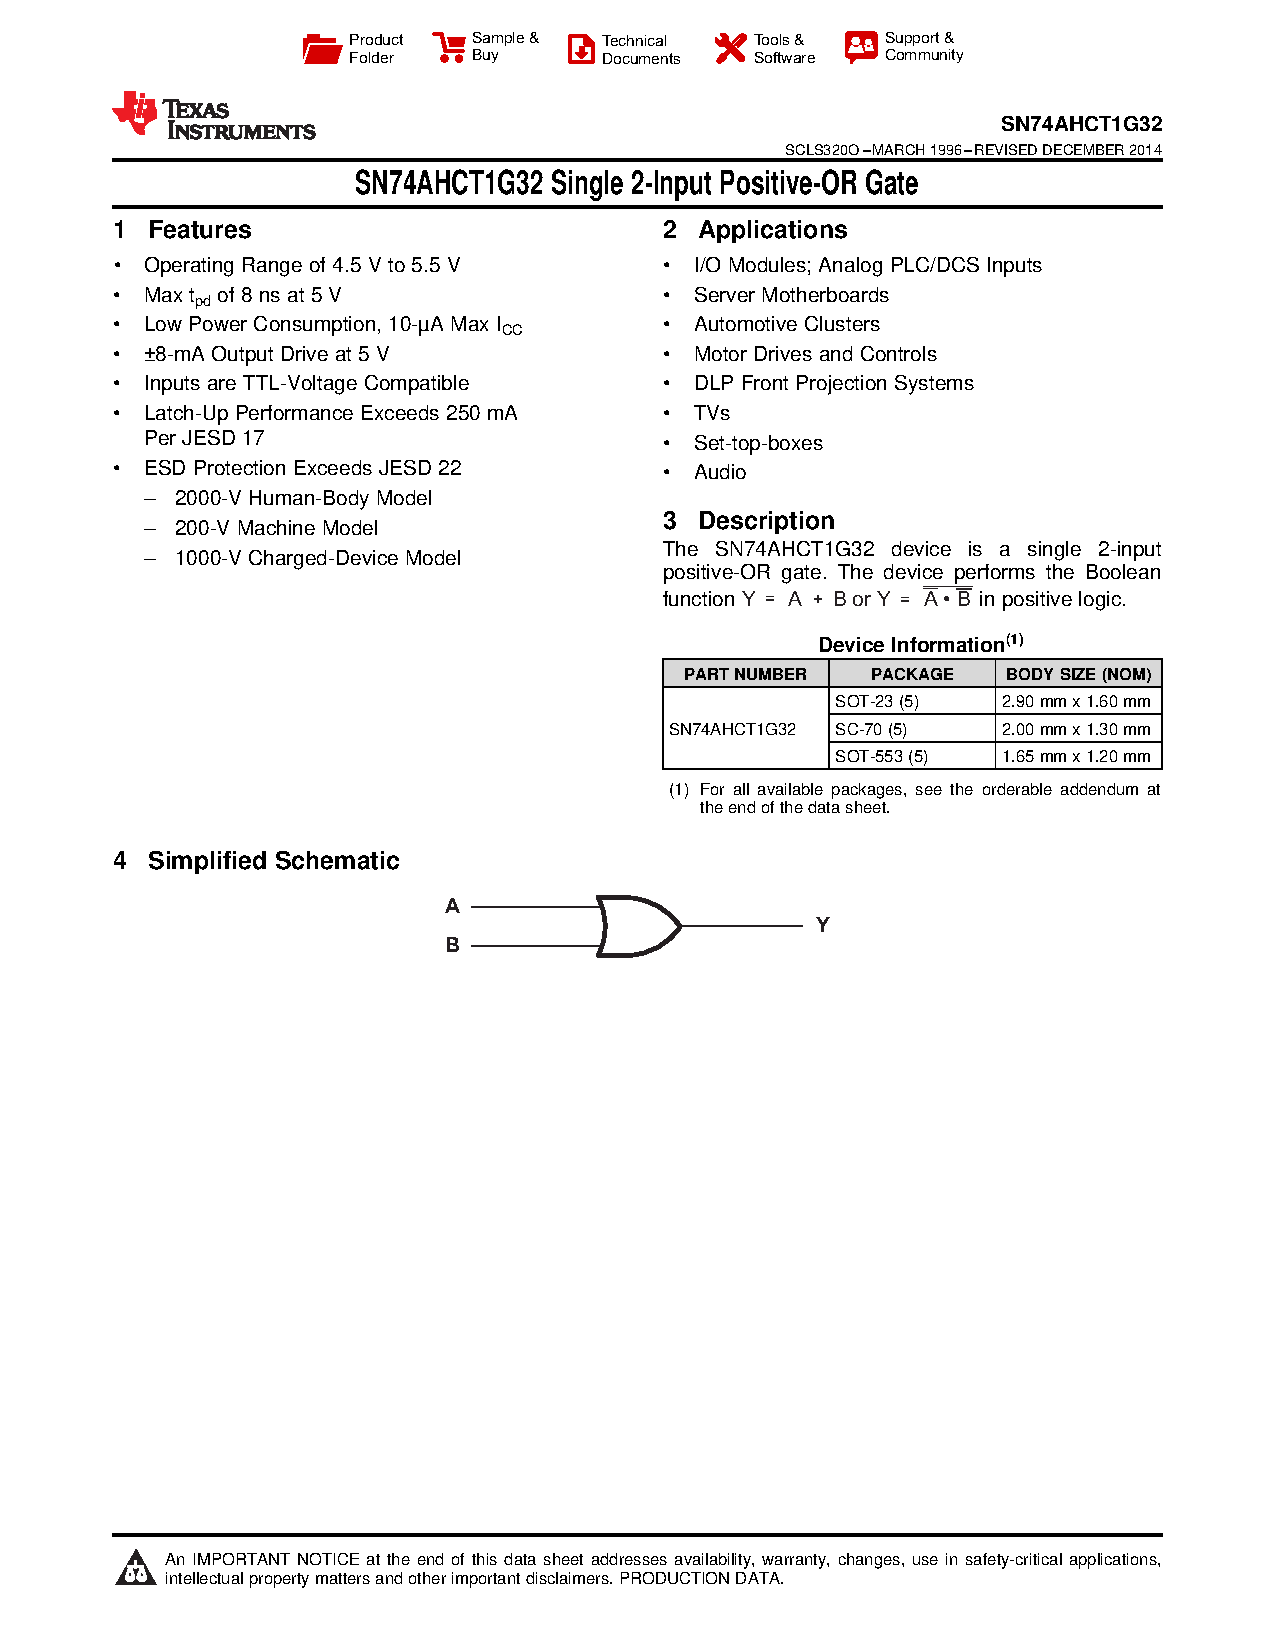
\includepdf[page=1,scale=\includepdfscale,pagecommand={\subsubsection{Porte Or Datasheet}\hypertarget{Or}{}}]{Gate OR.pdf}
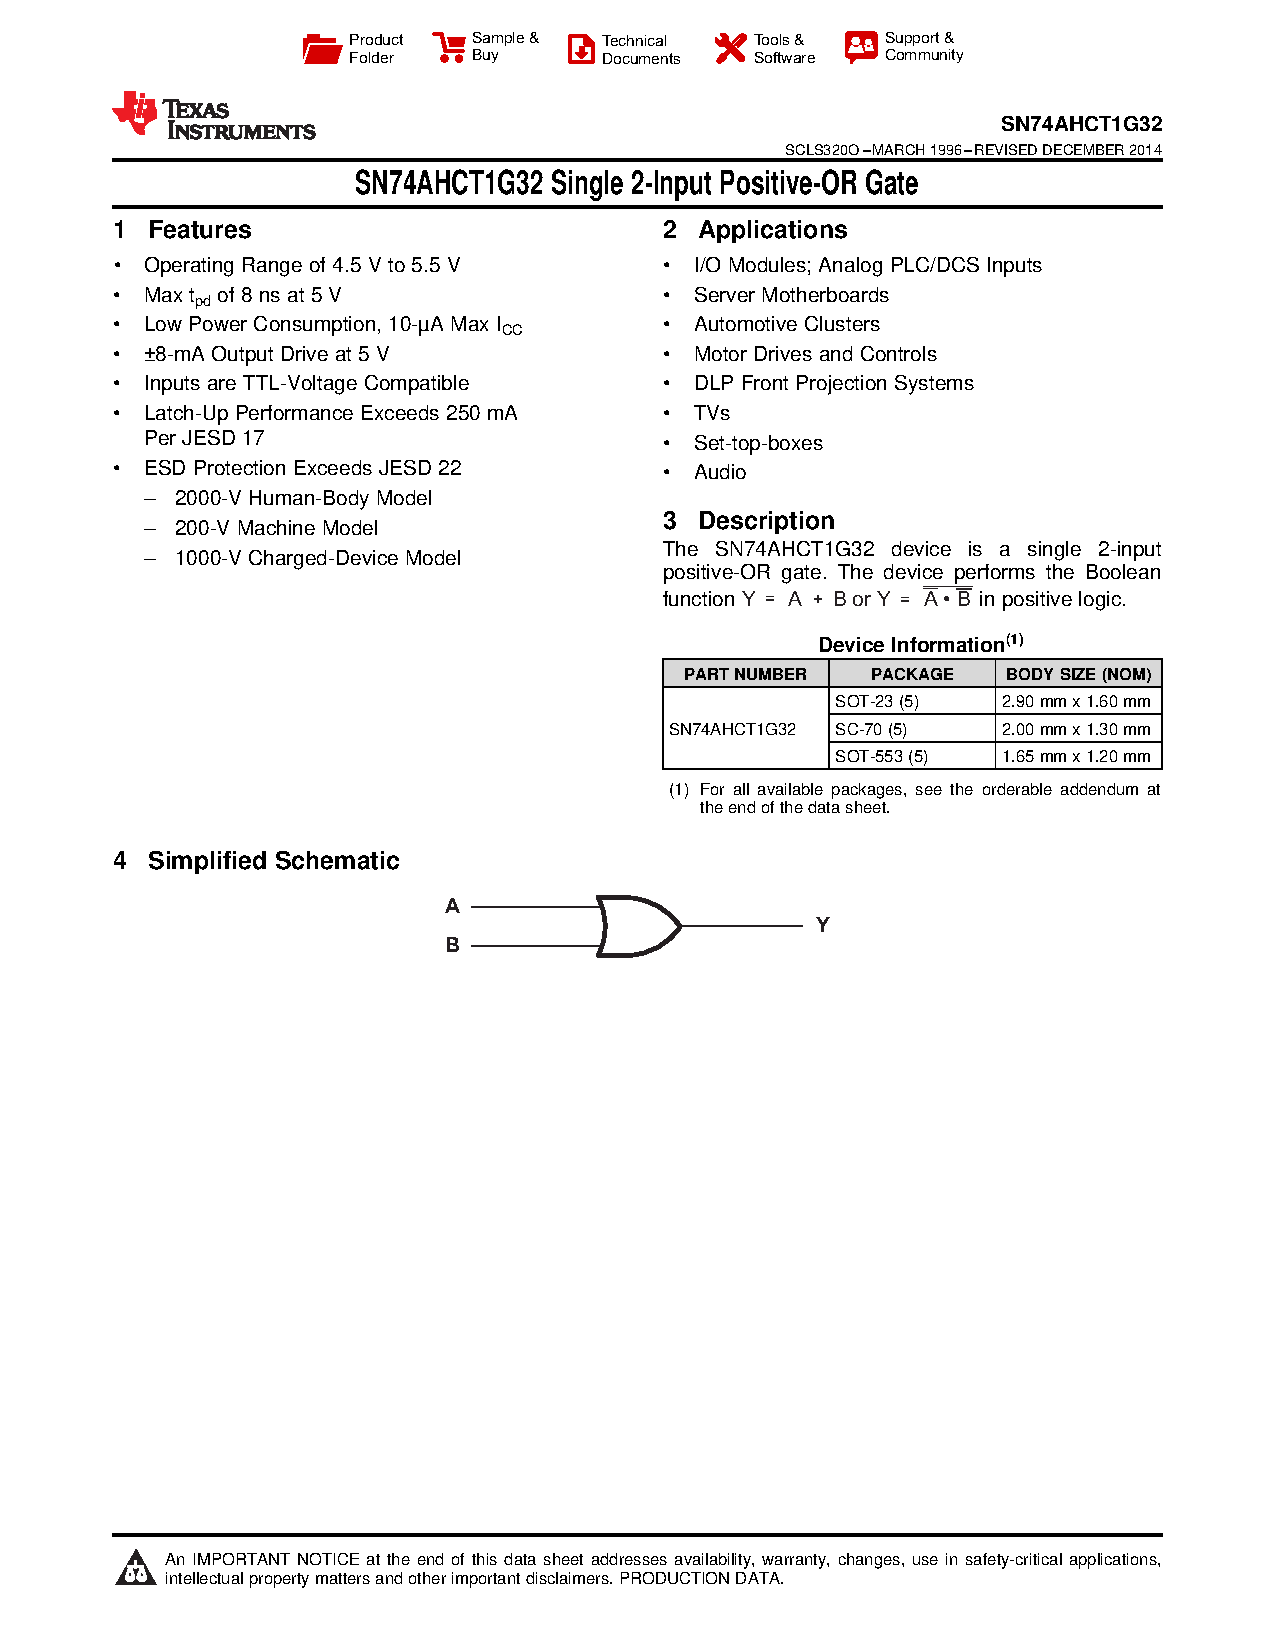
\includepdf[page=2-10,scale=\includepdfscale,pagecommand={}]{Gate OR.pdf}

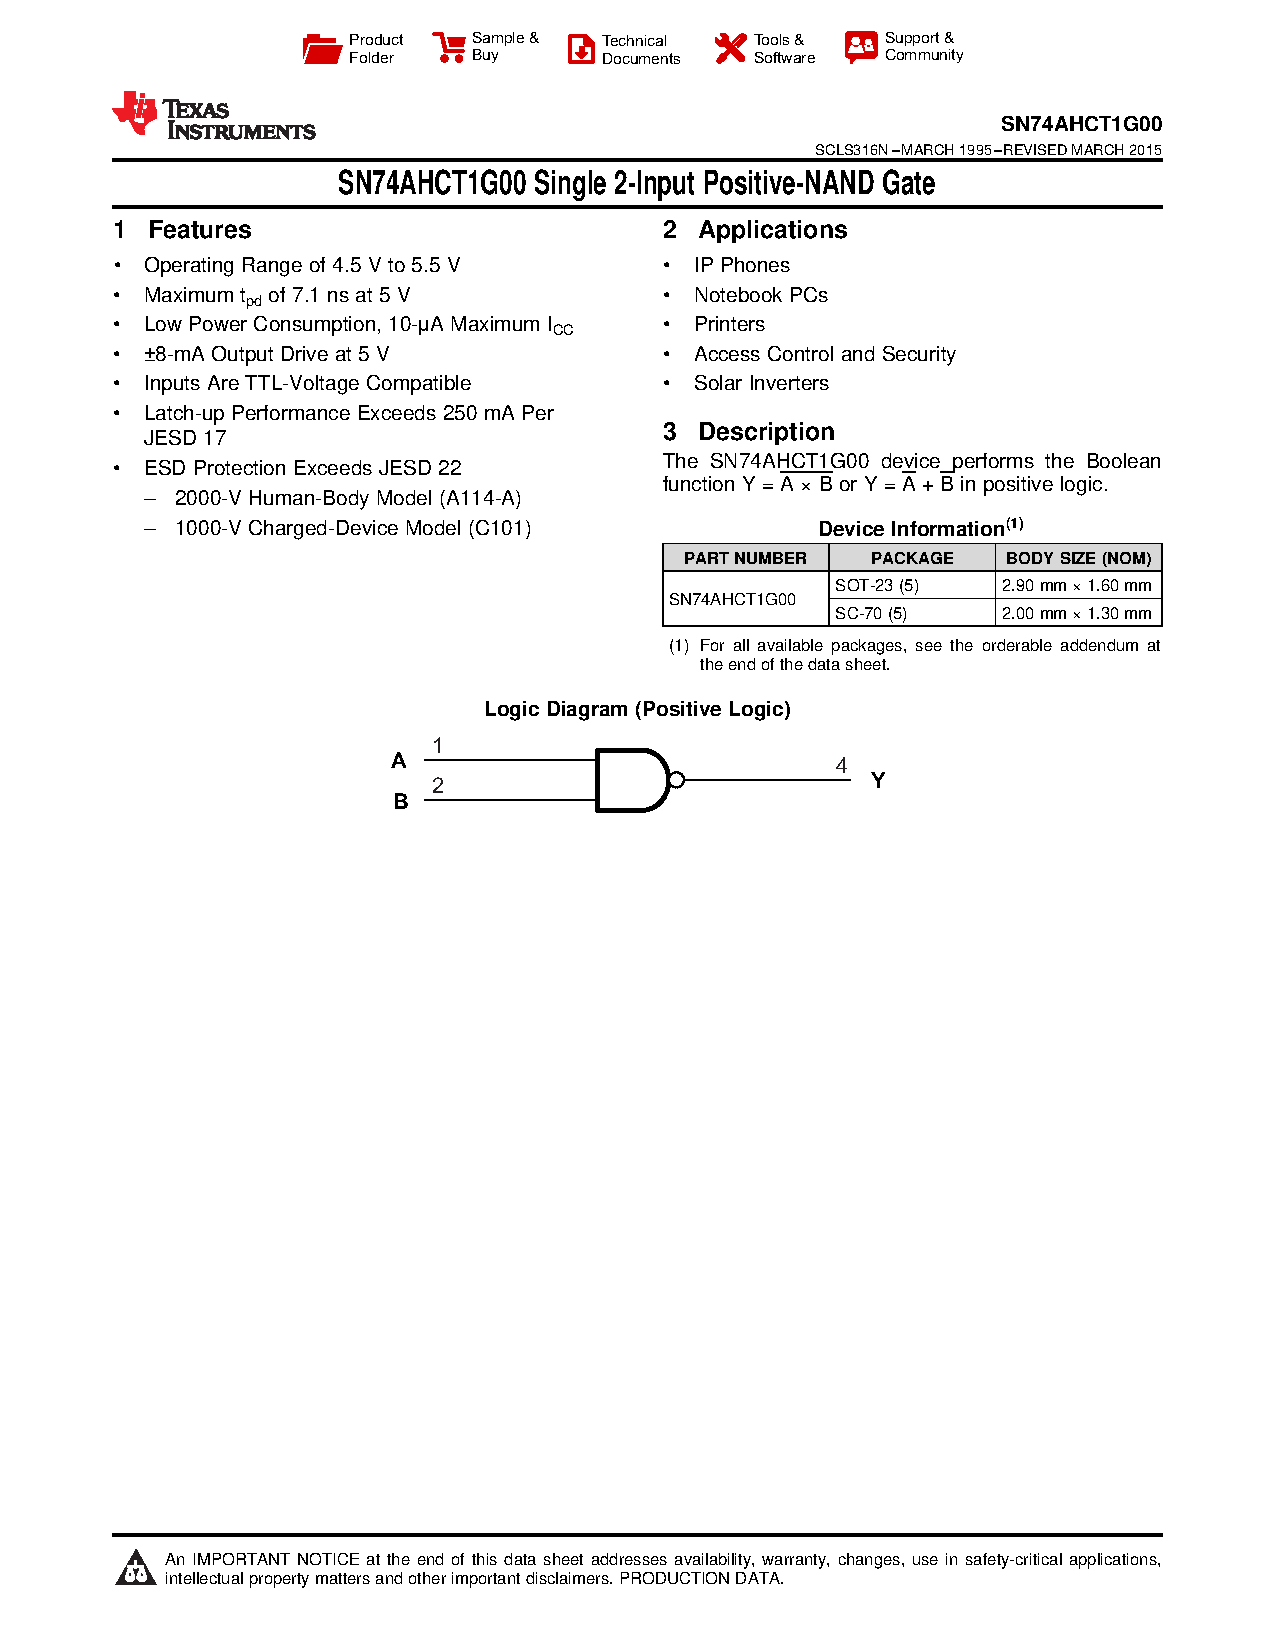
\includepdf[page=1,scale=\includepdfscale,pagecommand={\subsubsection{Porte NAnd Datasheet}\hypertarget{NAnd}{}}]{Gate NAND.pdf}
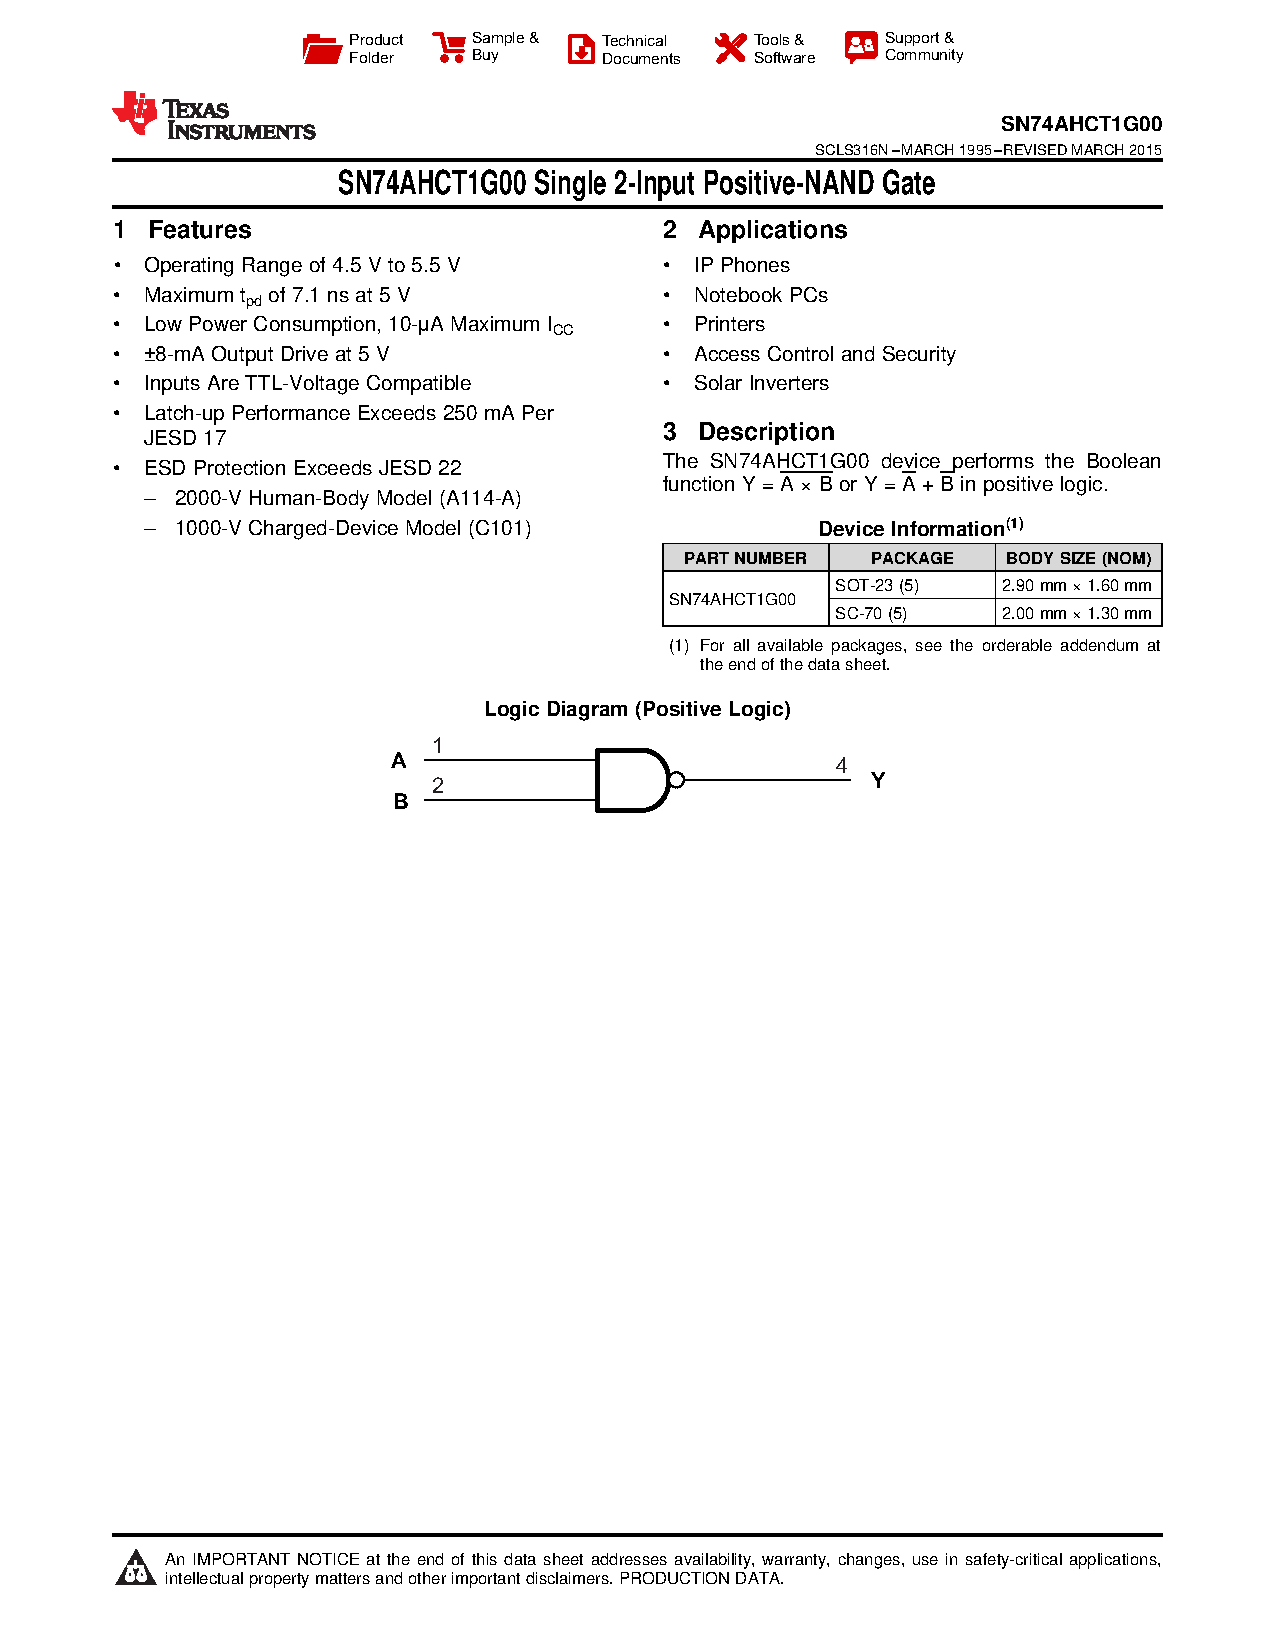
\includepdf[page=2-11,scale=\includepdfscale,pagecommand={}]{Gate NAND.pdf}

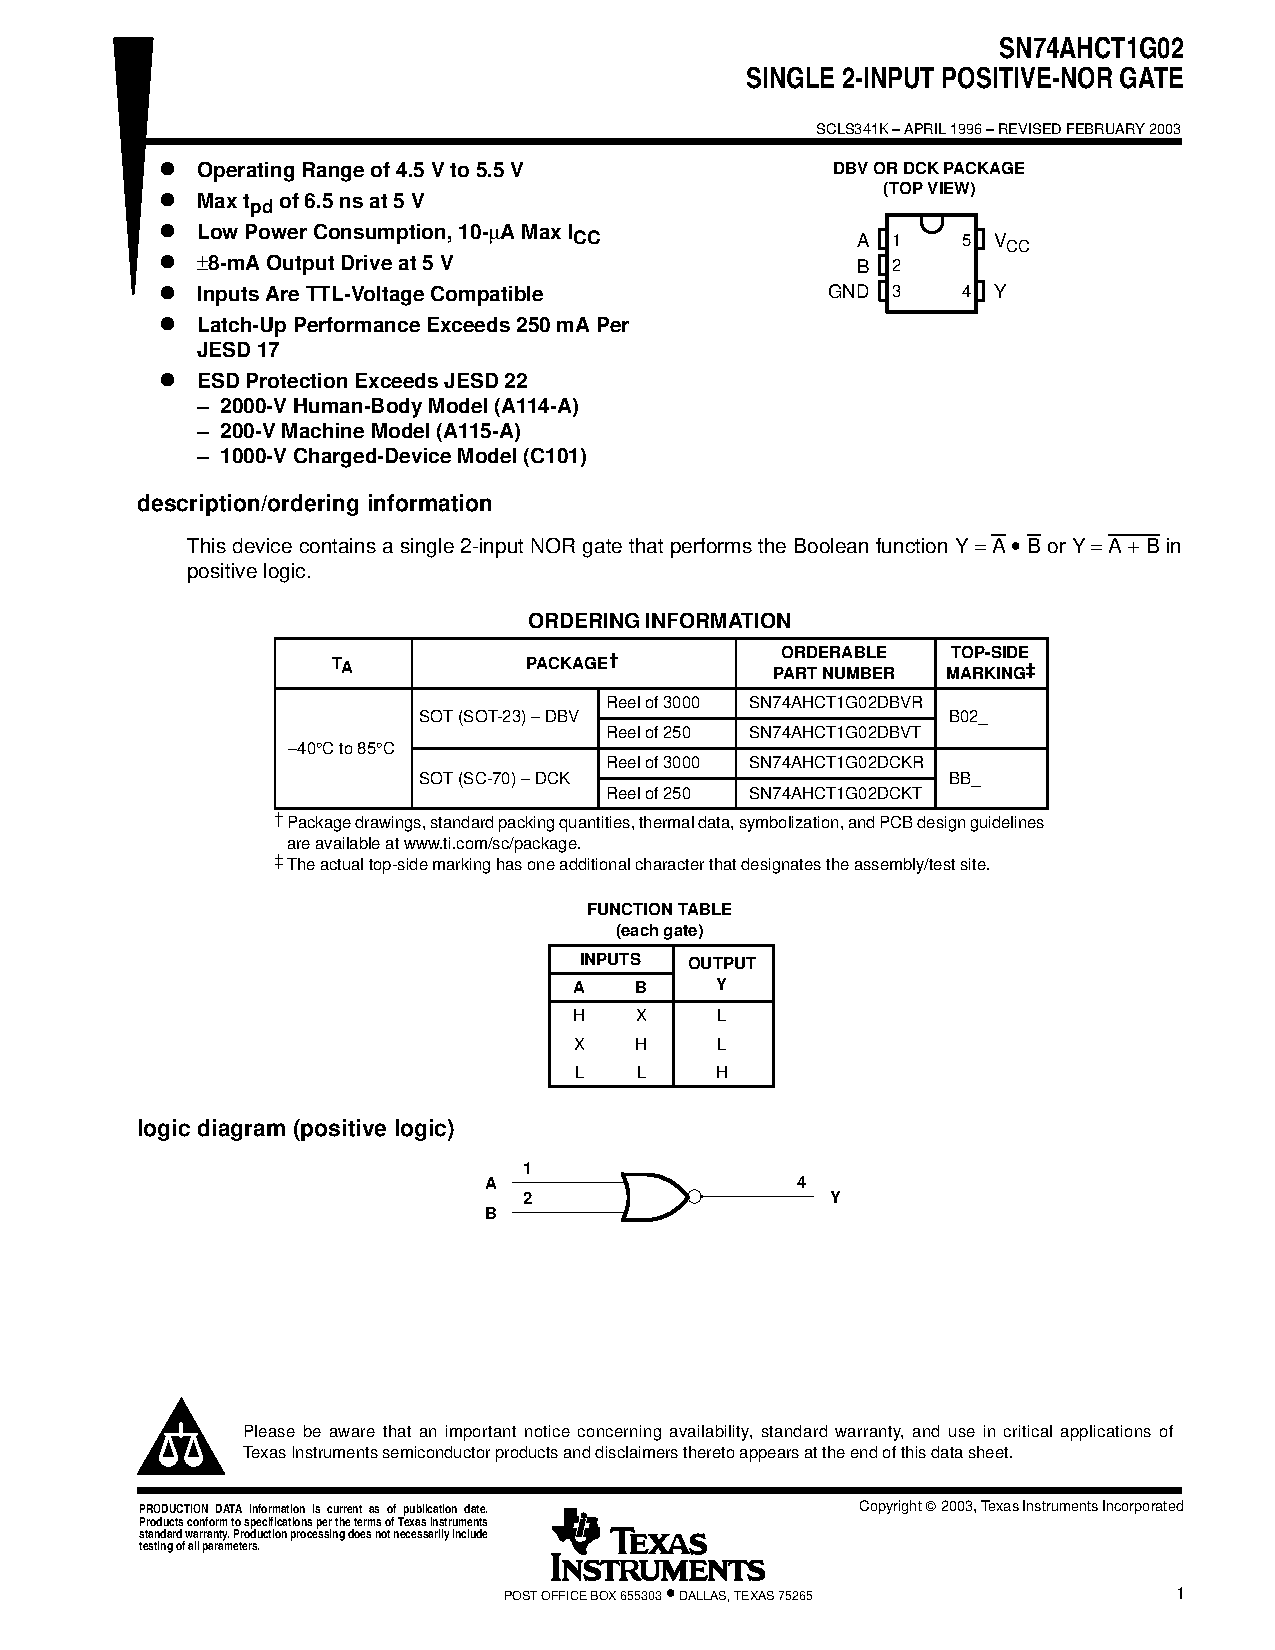
\includepdf[page=1,scale=\includepdfscale,pagecommand={\subsubsection{Porte NOr Datasheet}\hypertarget{NOr}{}}]{Gate NOR.pdf}
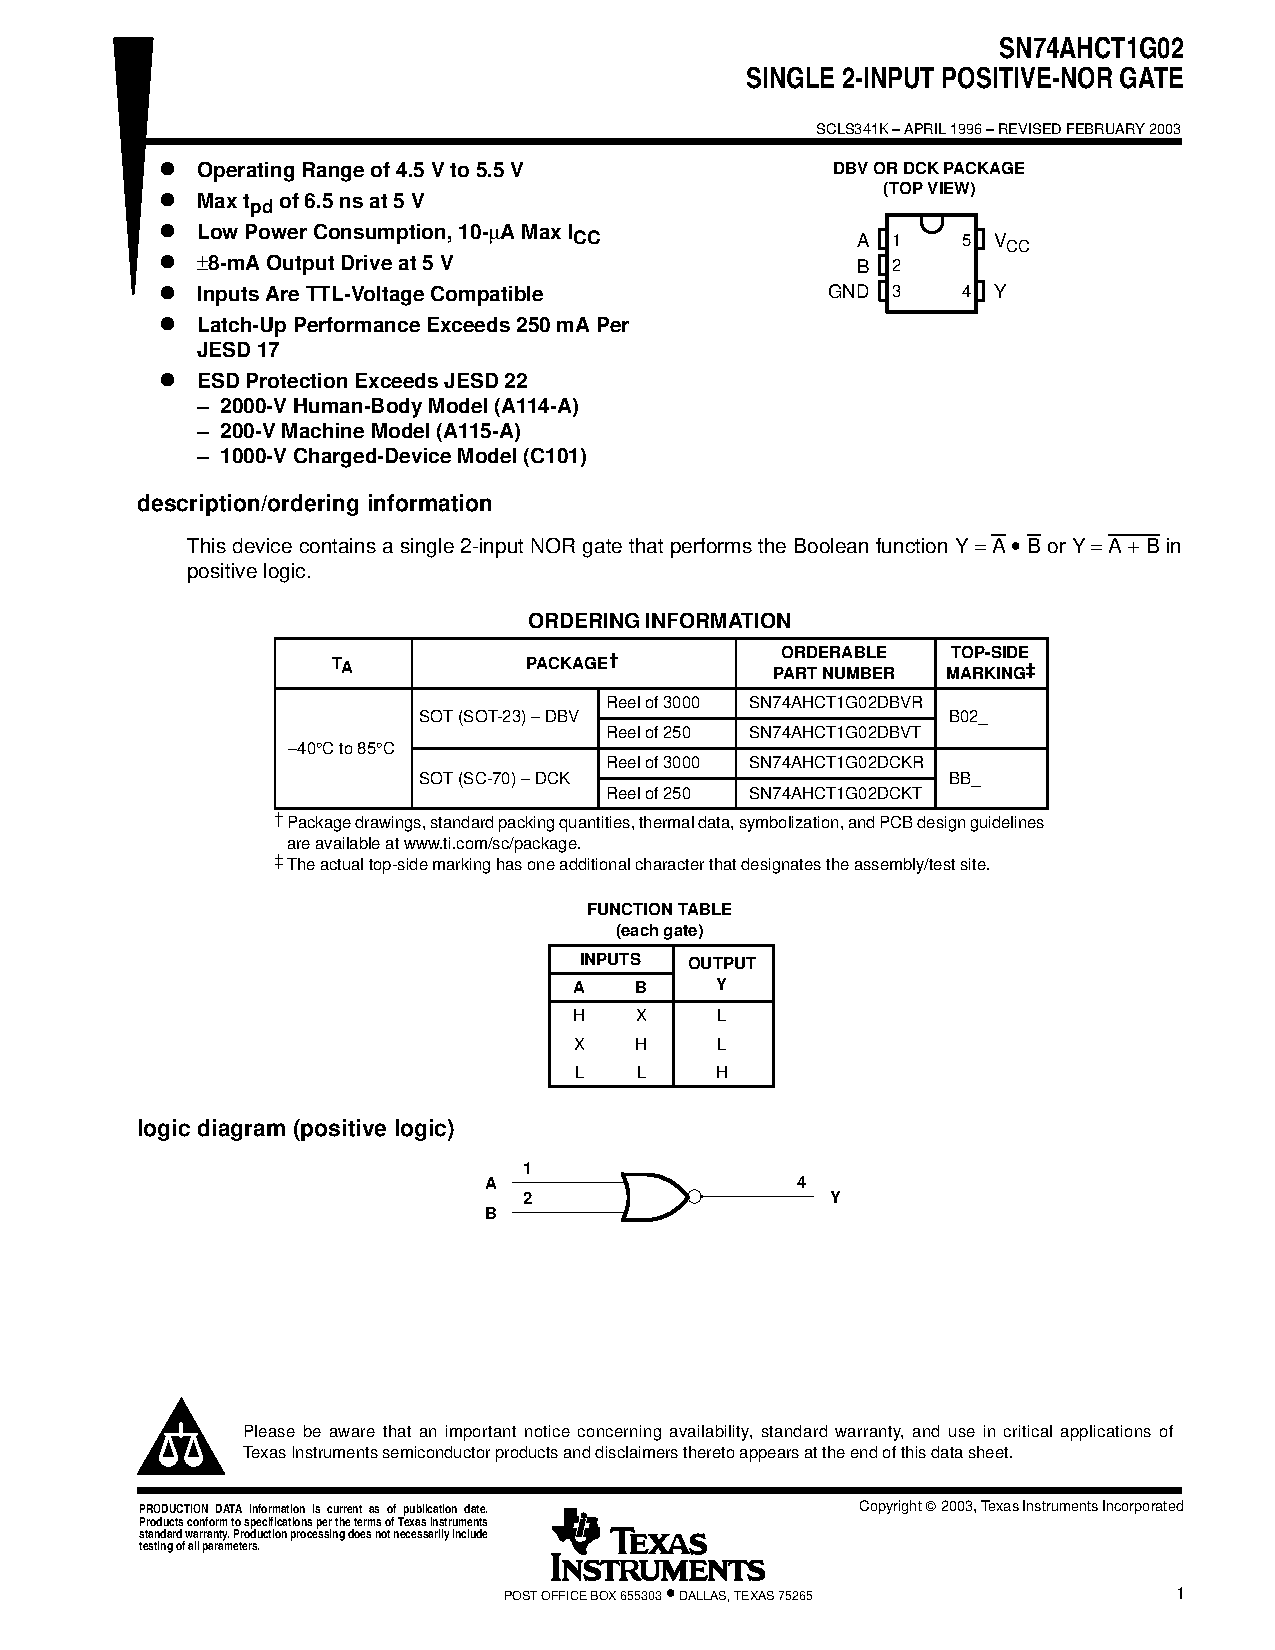
\includepdf[page=2-4,scale=\includepdfscale,pagecommand={}]{Gate NOR.pdf}

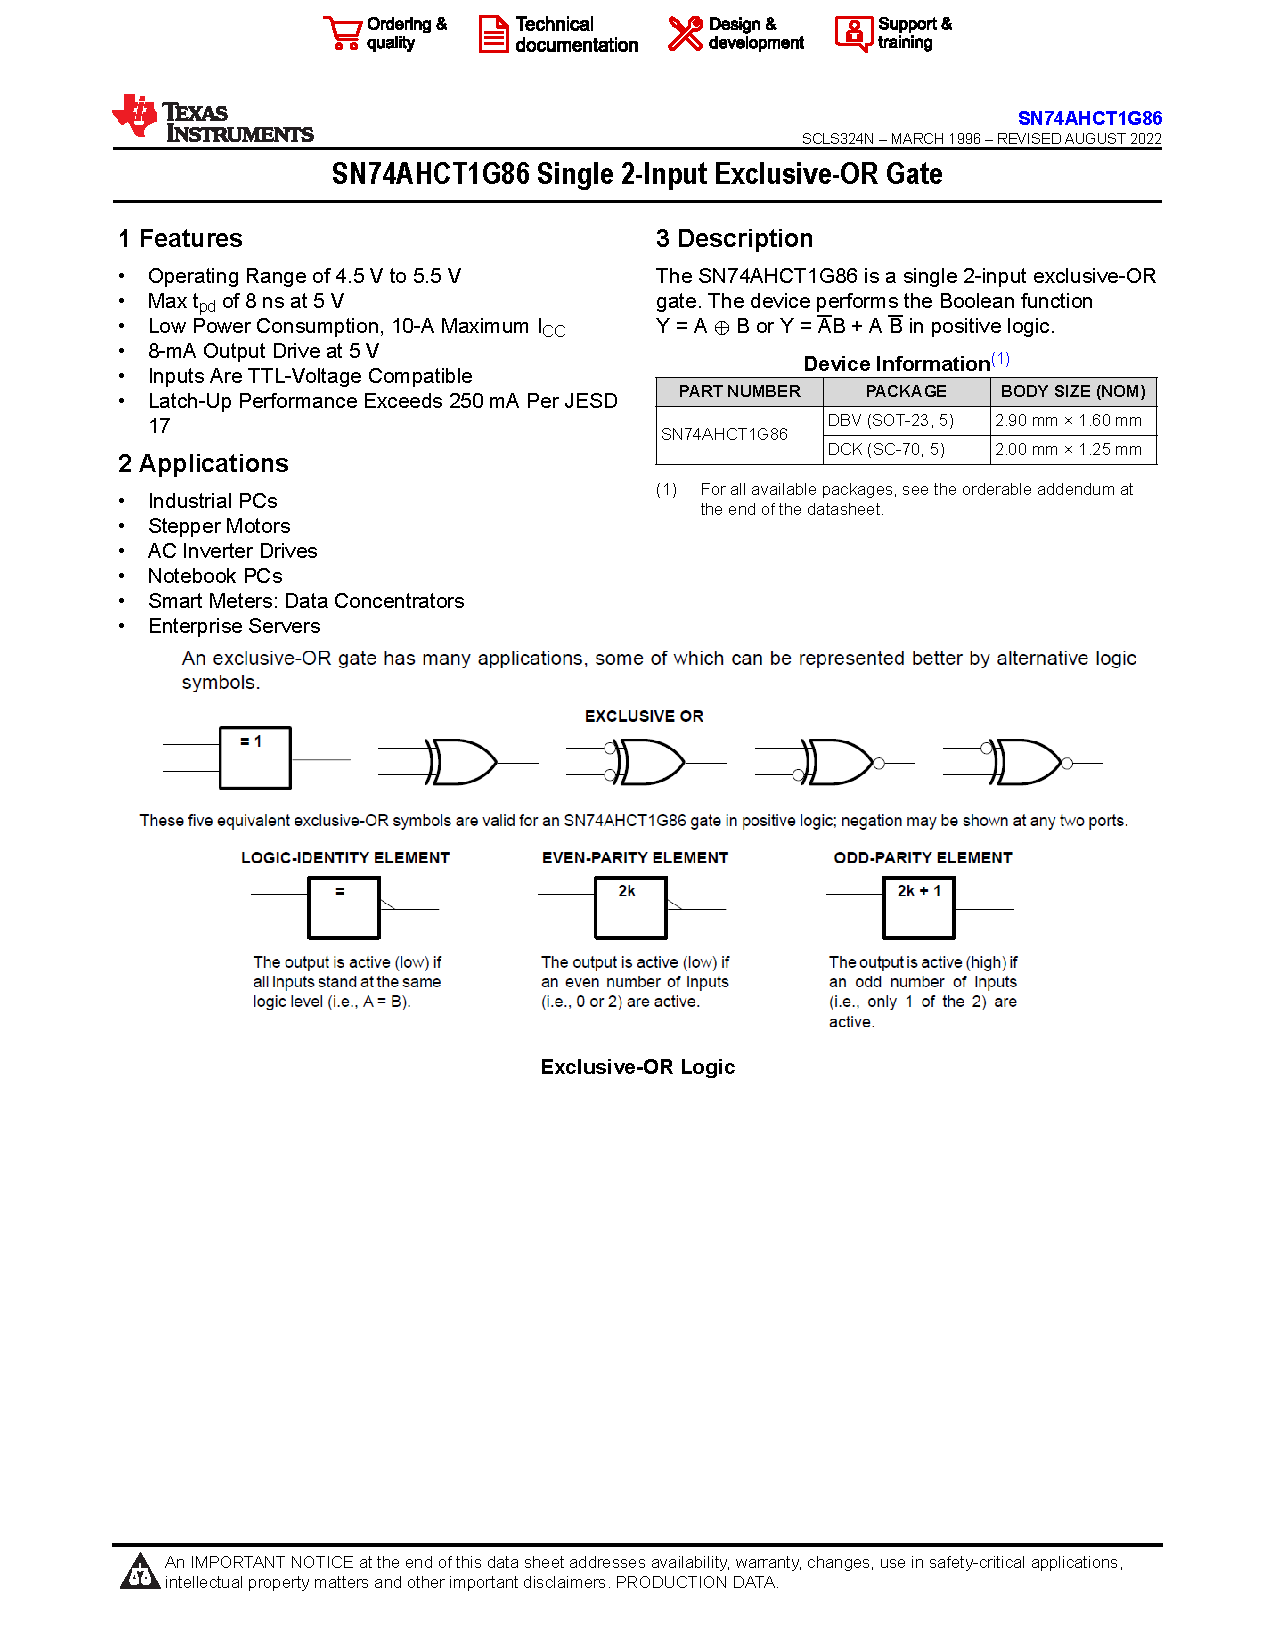
\includepdf[page=1,scale=\includepdfscale,pagecommand={\subsubsection{Porte XOr Datasheet}\hypertarget{XOr}{}}]{Gate XOR.pdf}
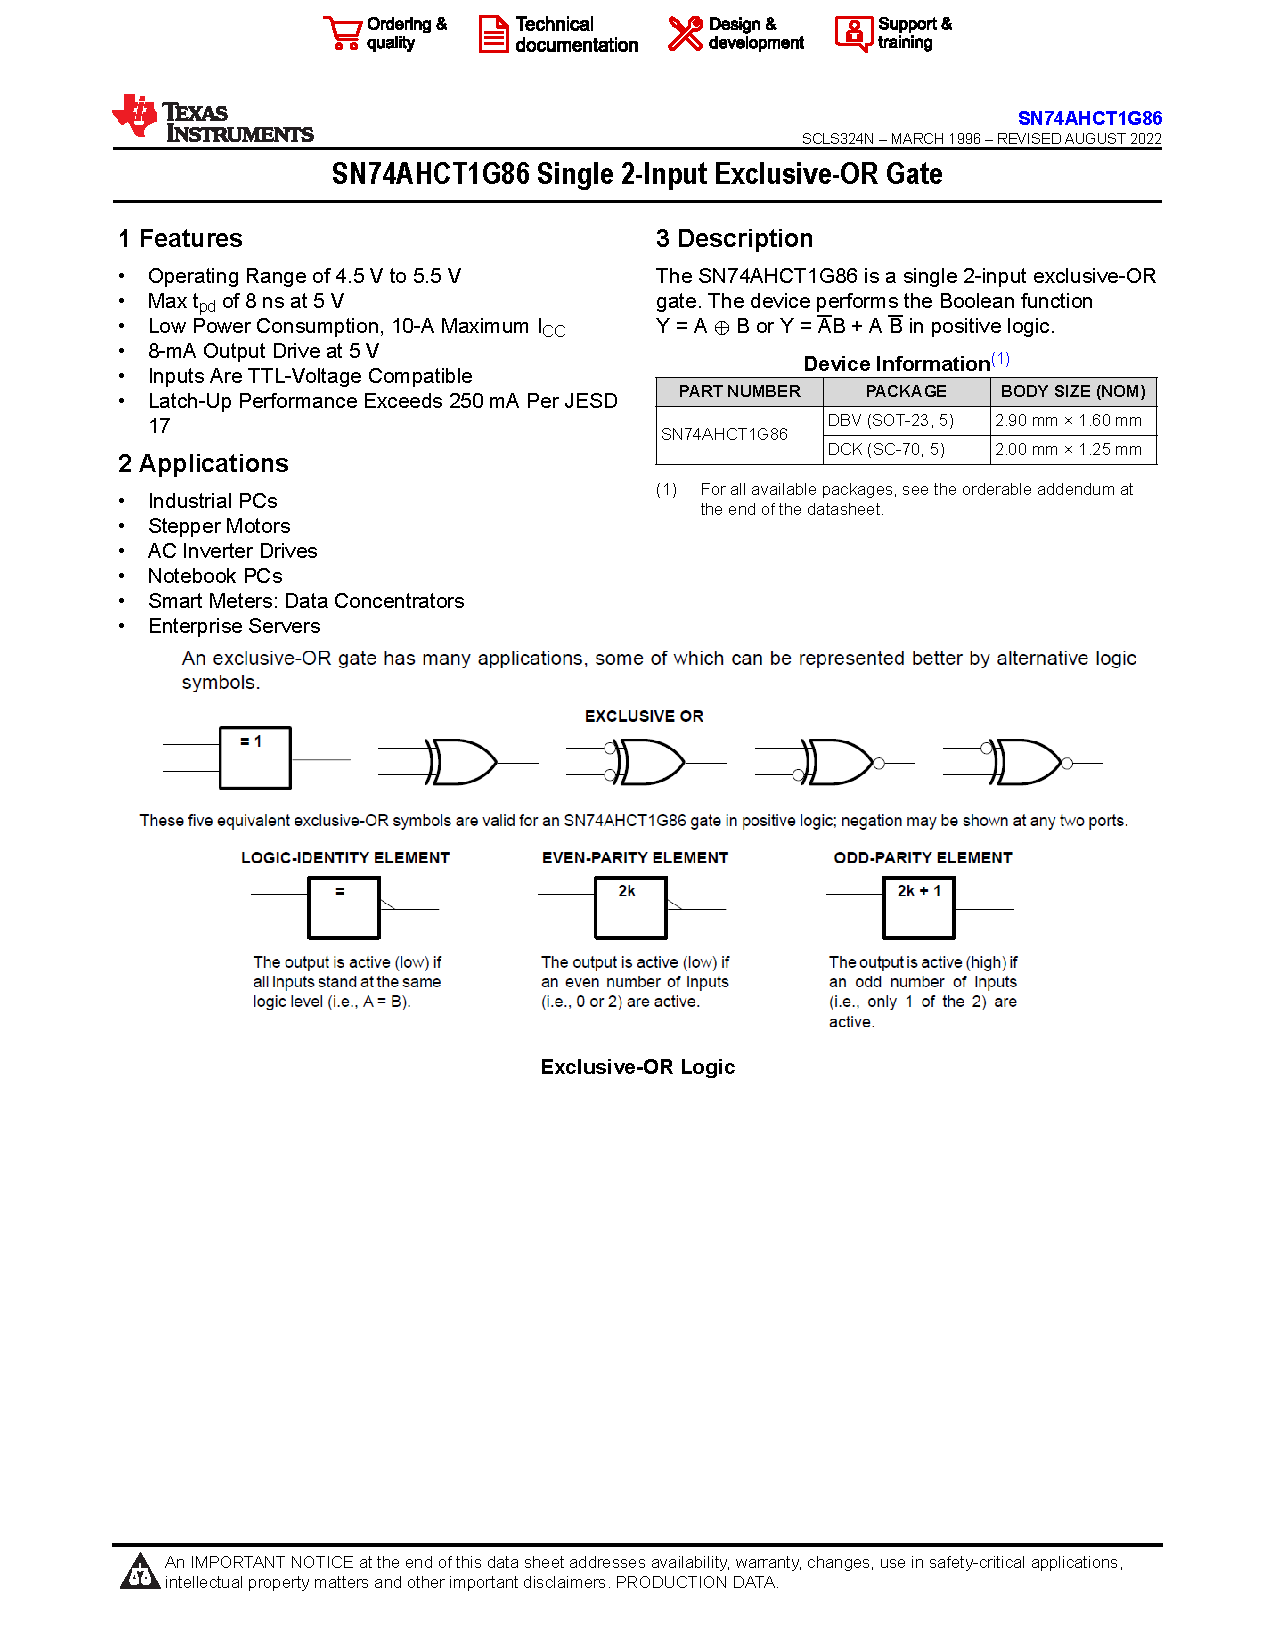
\includepdf[page=2-12,scale=\includepdfscale,pagecommand={}]{Gate XOR.pdf}

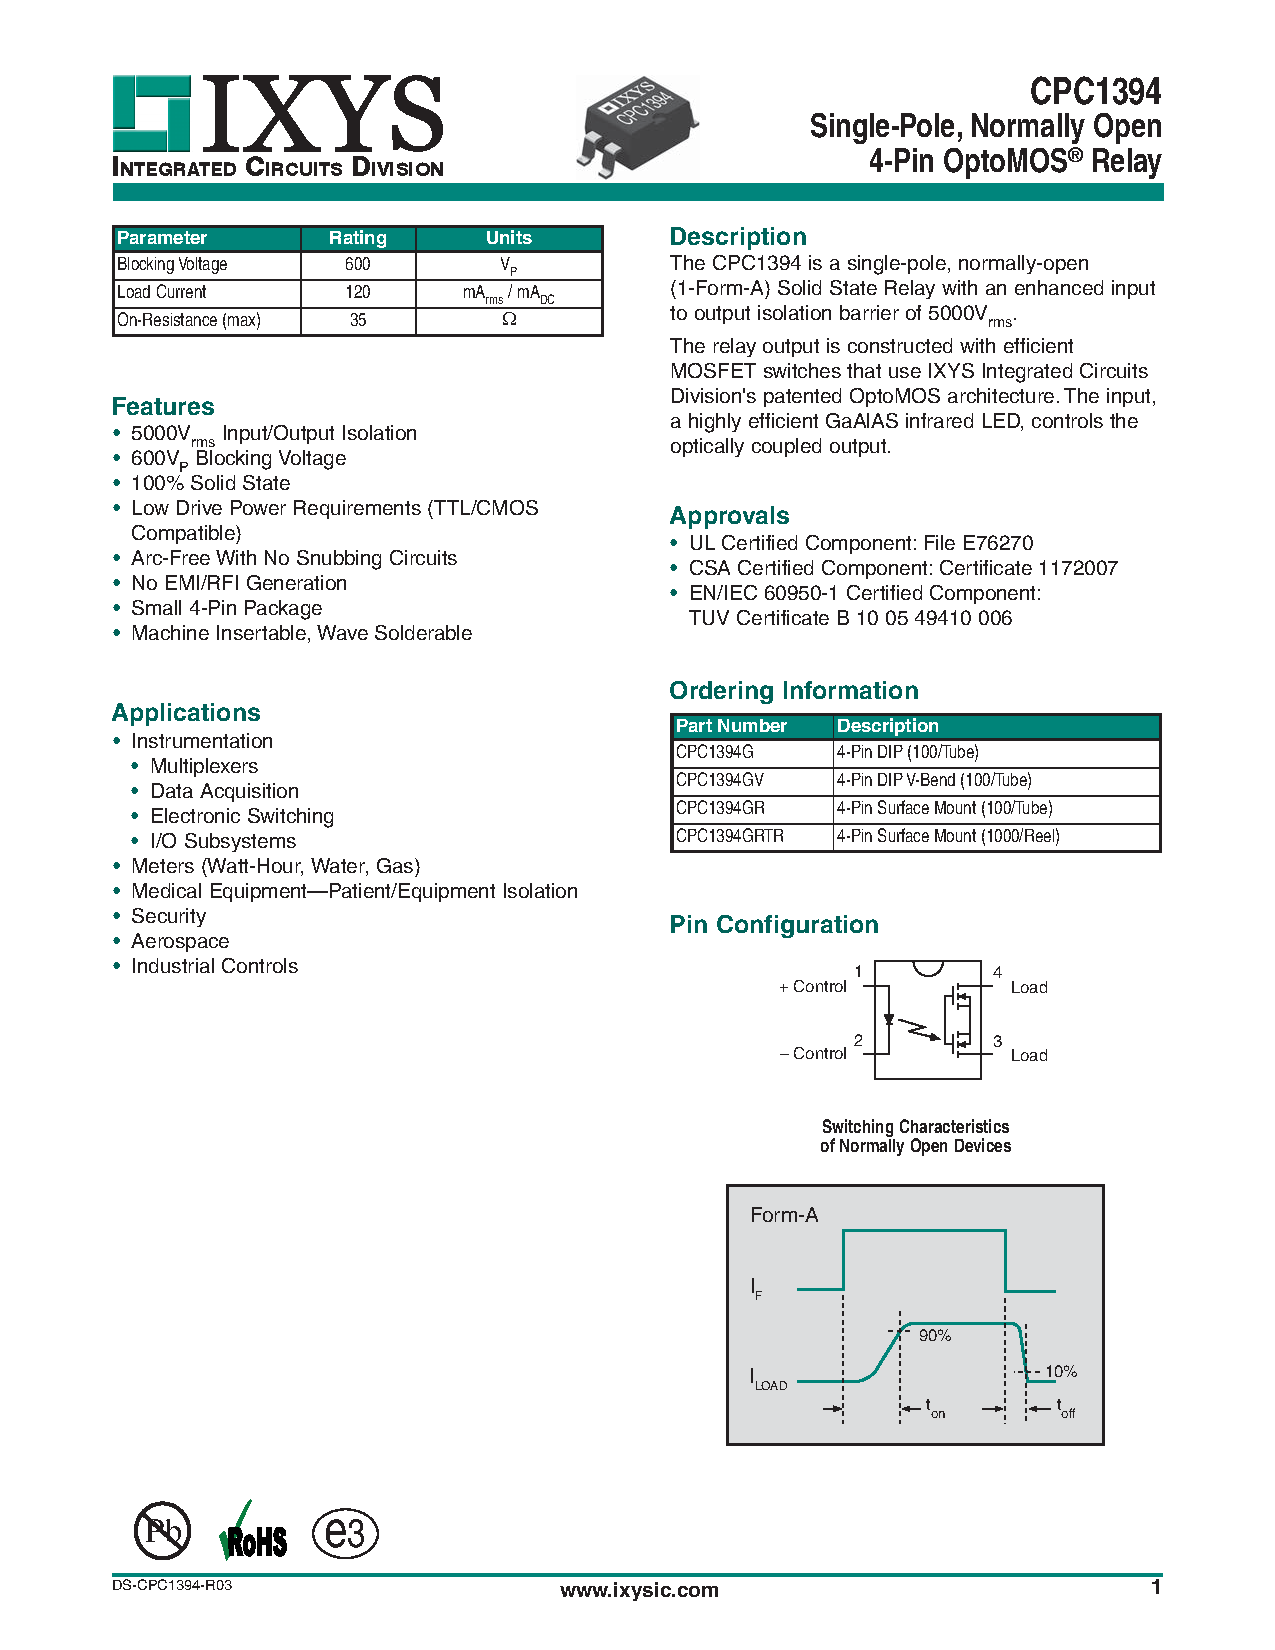
\includepdf[page=1,scale=\includepdfscale,pagecommand={\subsection{Solid State Relay Datasheet}\hypertarget{SSR}{}}]{SSR.pdf}
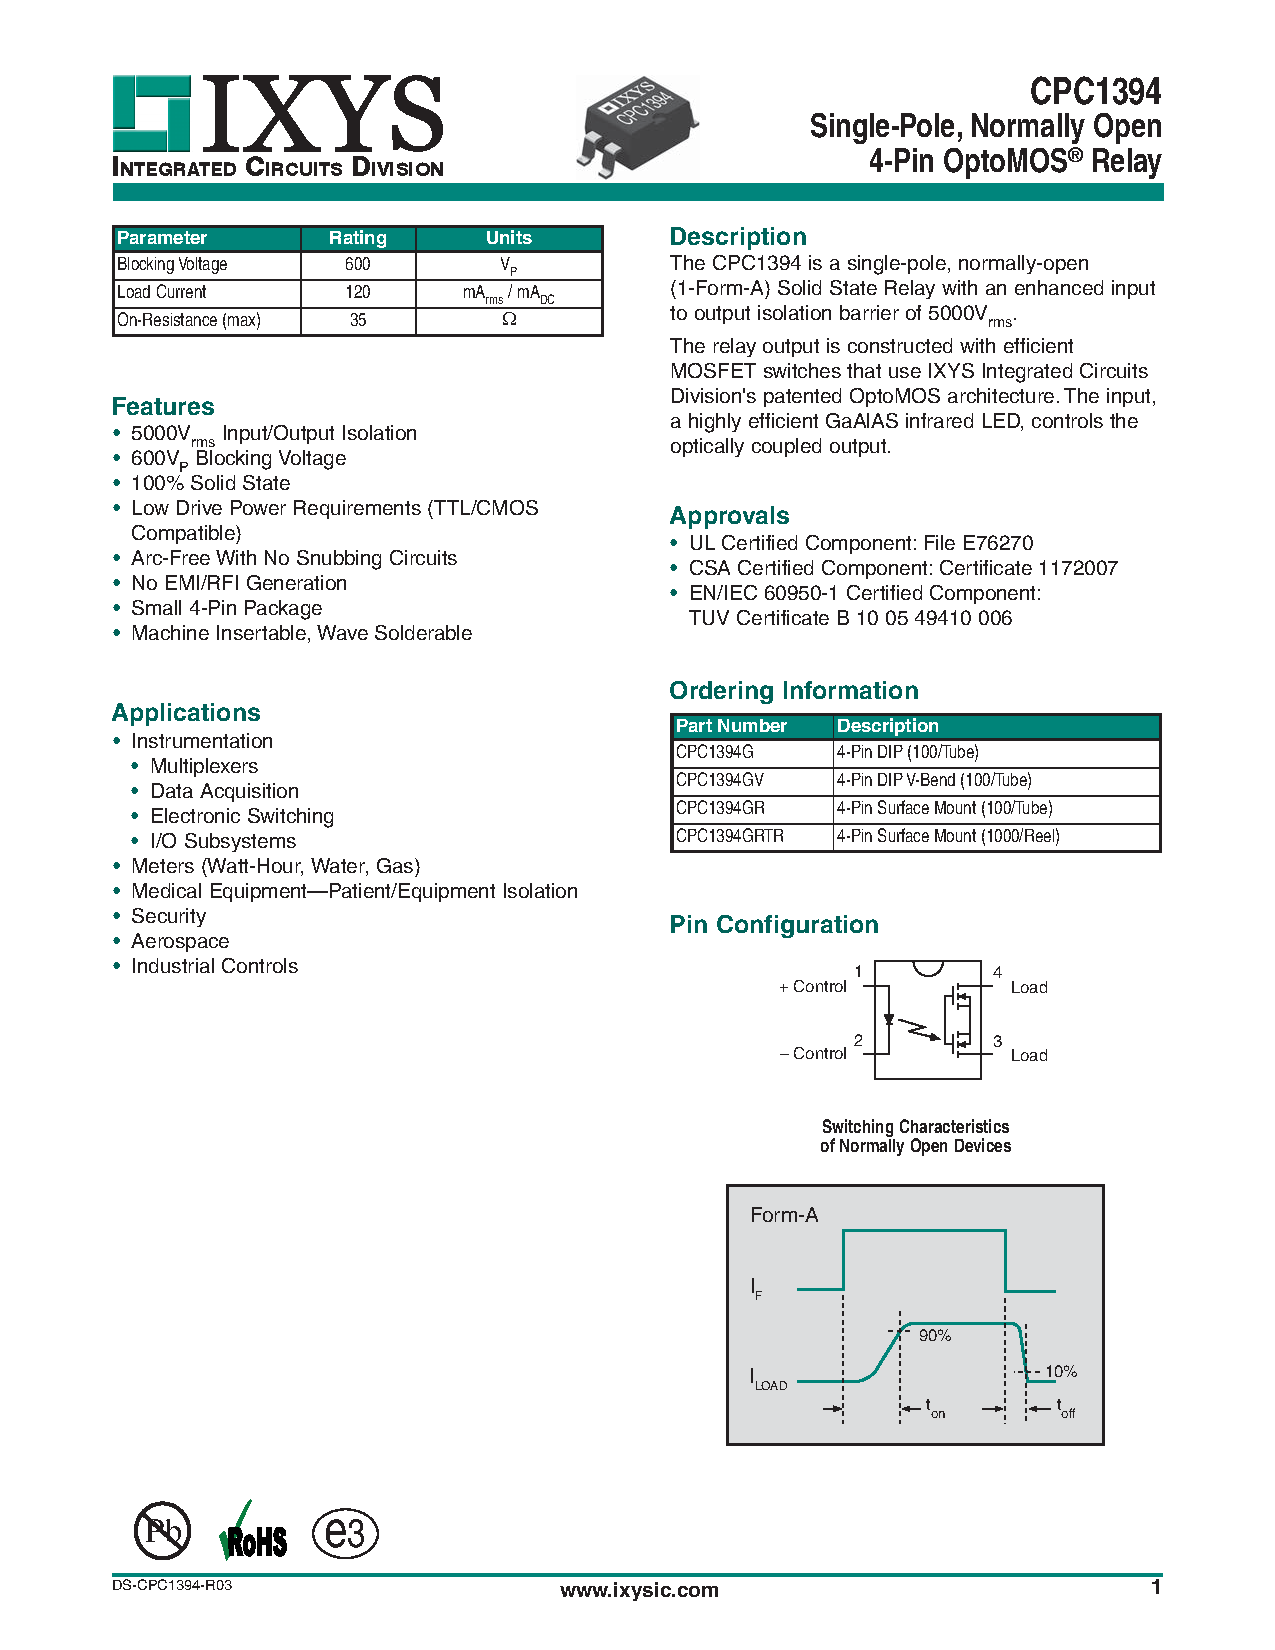
\includepdf[page=2-5,scale=\includepdfscale,pagecommand={}]{SSR.pdf}

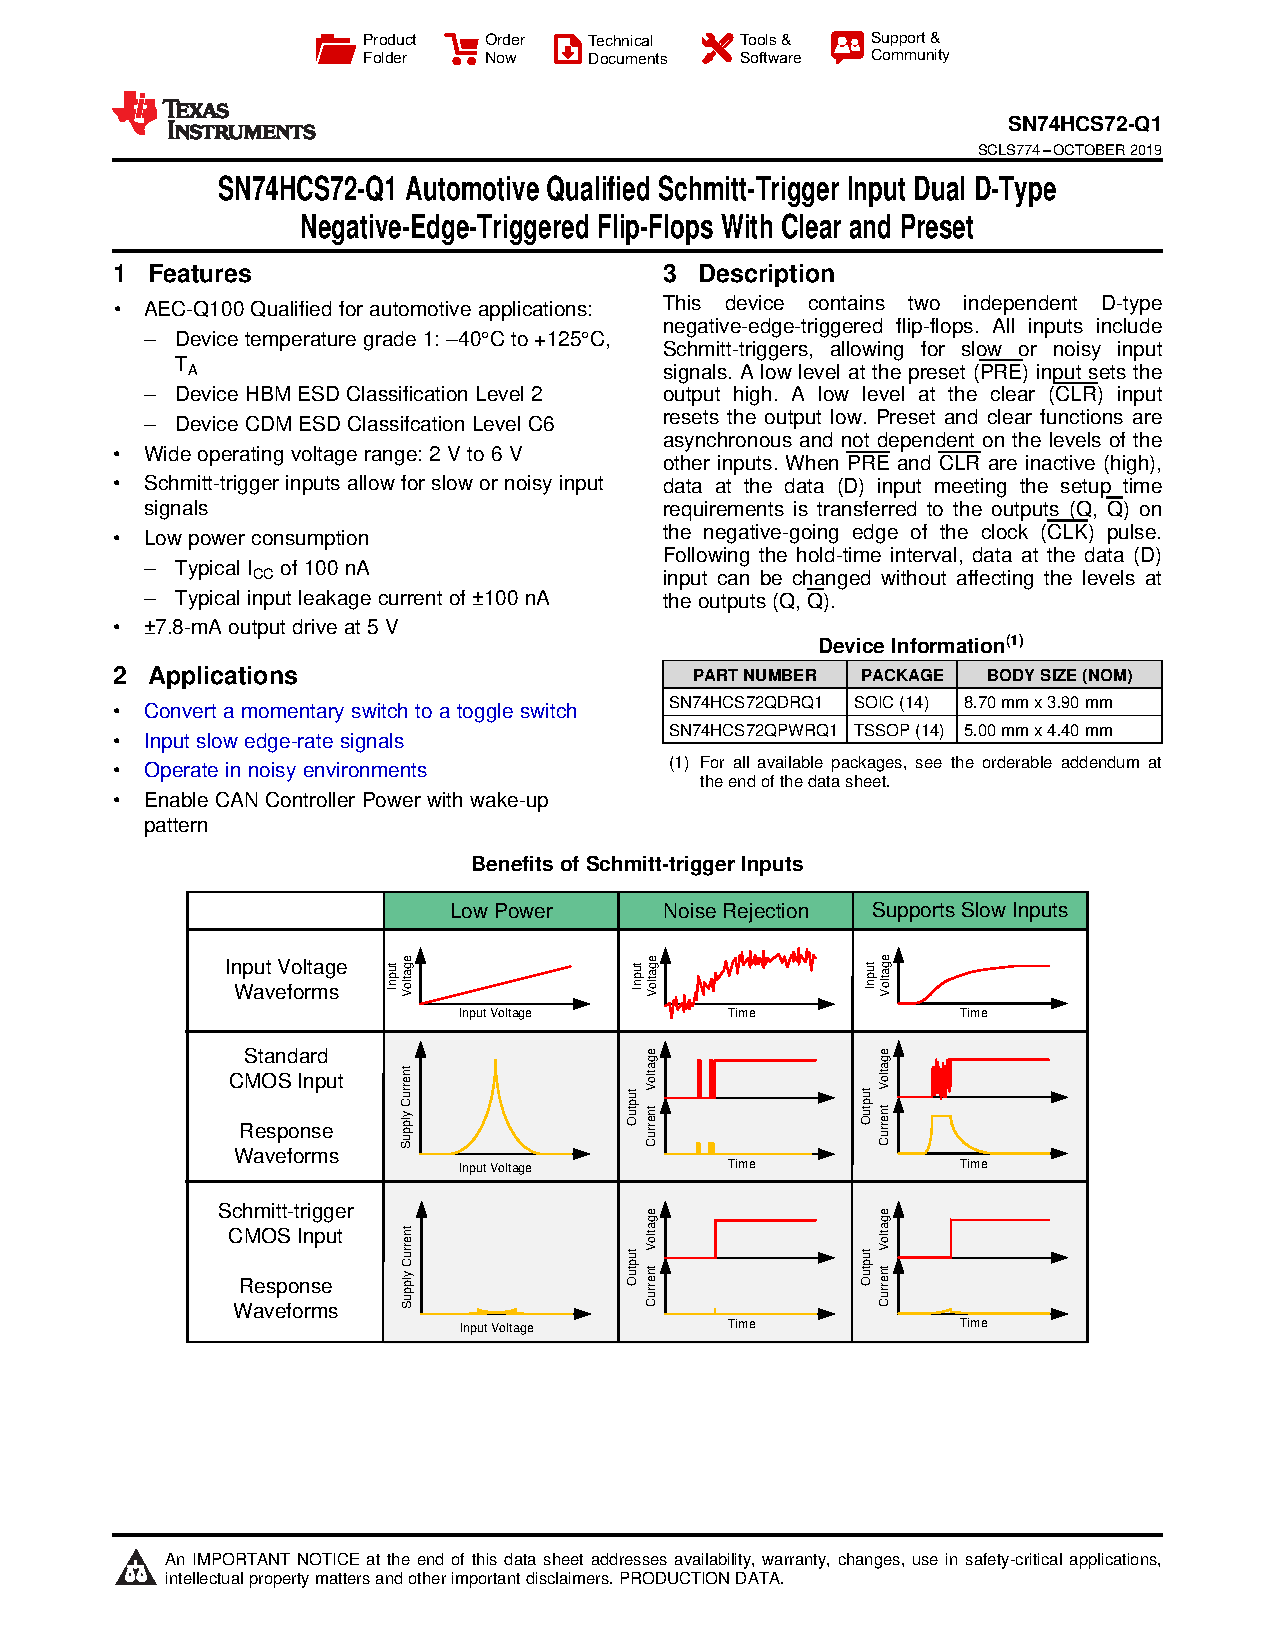
\includepdf[page=1,scale=\includepdfscale,pagecommand={\subsection{Bascule D Datasheet}\hypertarget{DLatch}{}}]{D Latch.pdf}
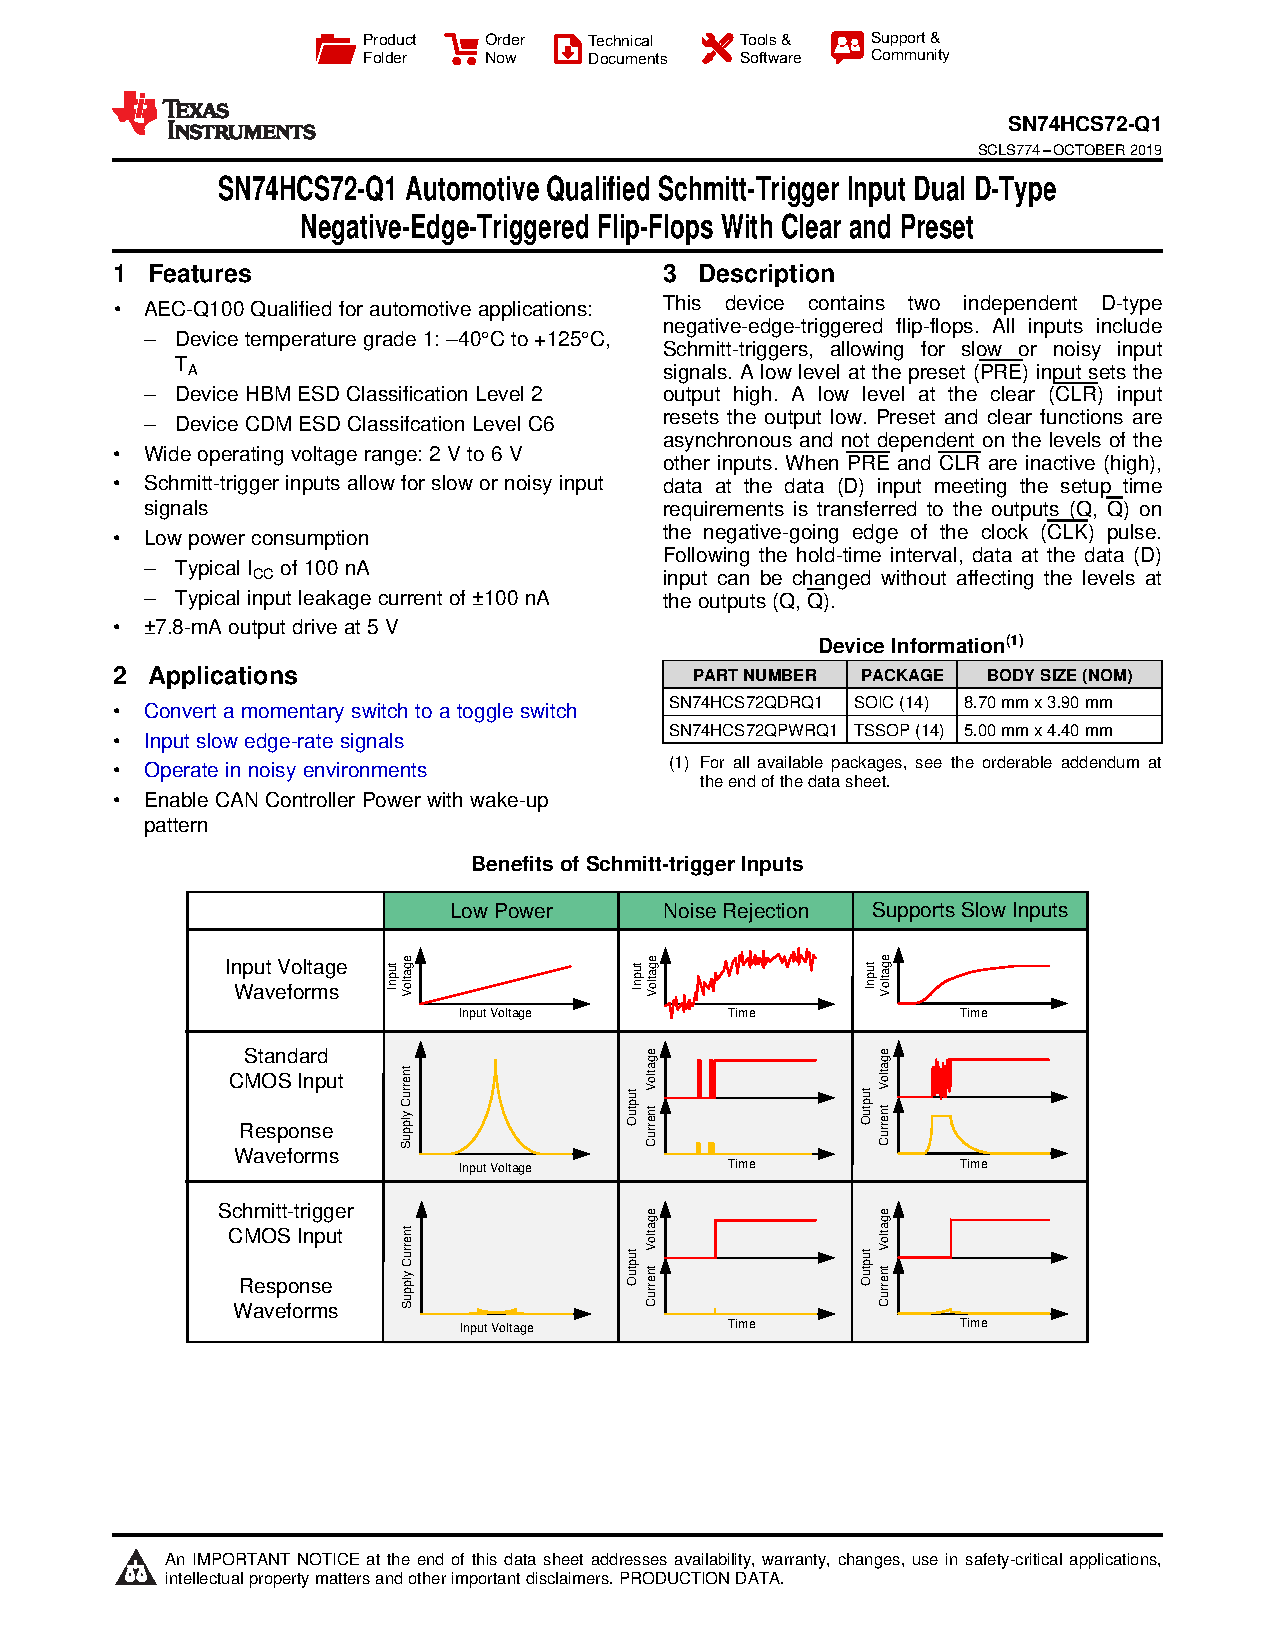
\includepdf[page=2-14,scale=\includepdfscale,pagecommand={}]{D Latch.pdf}

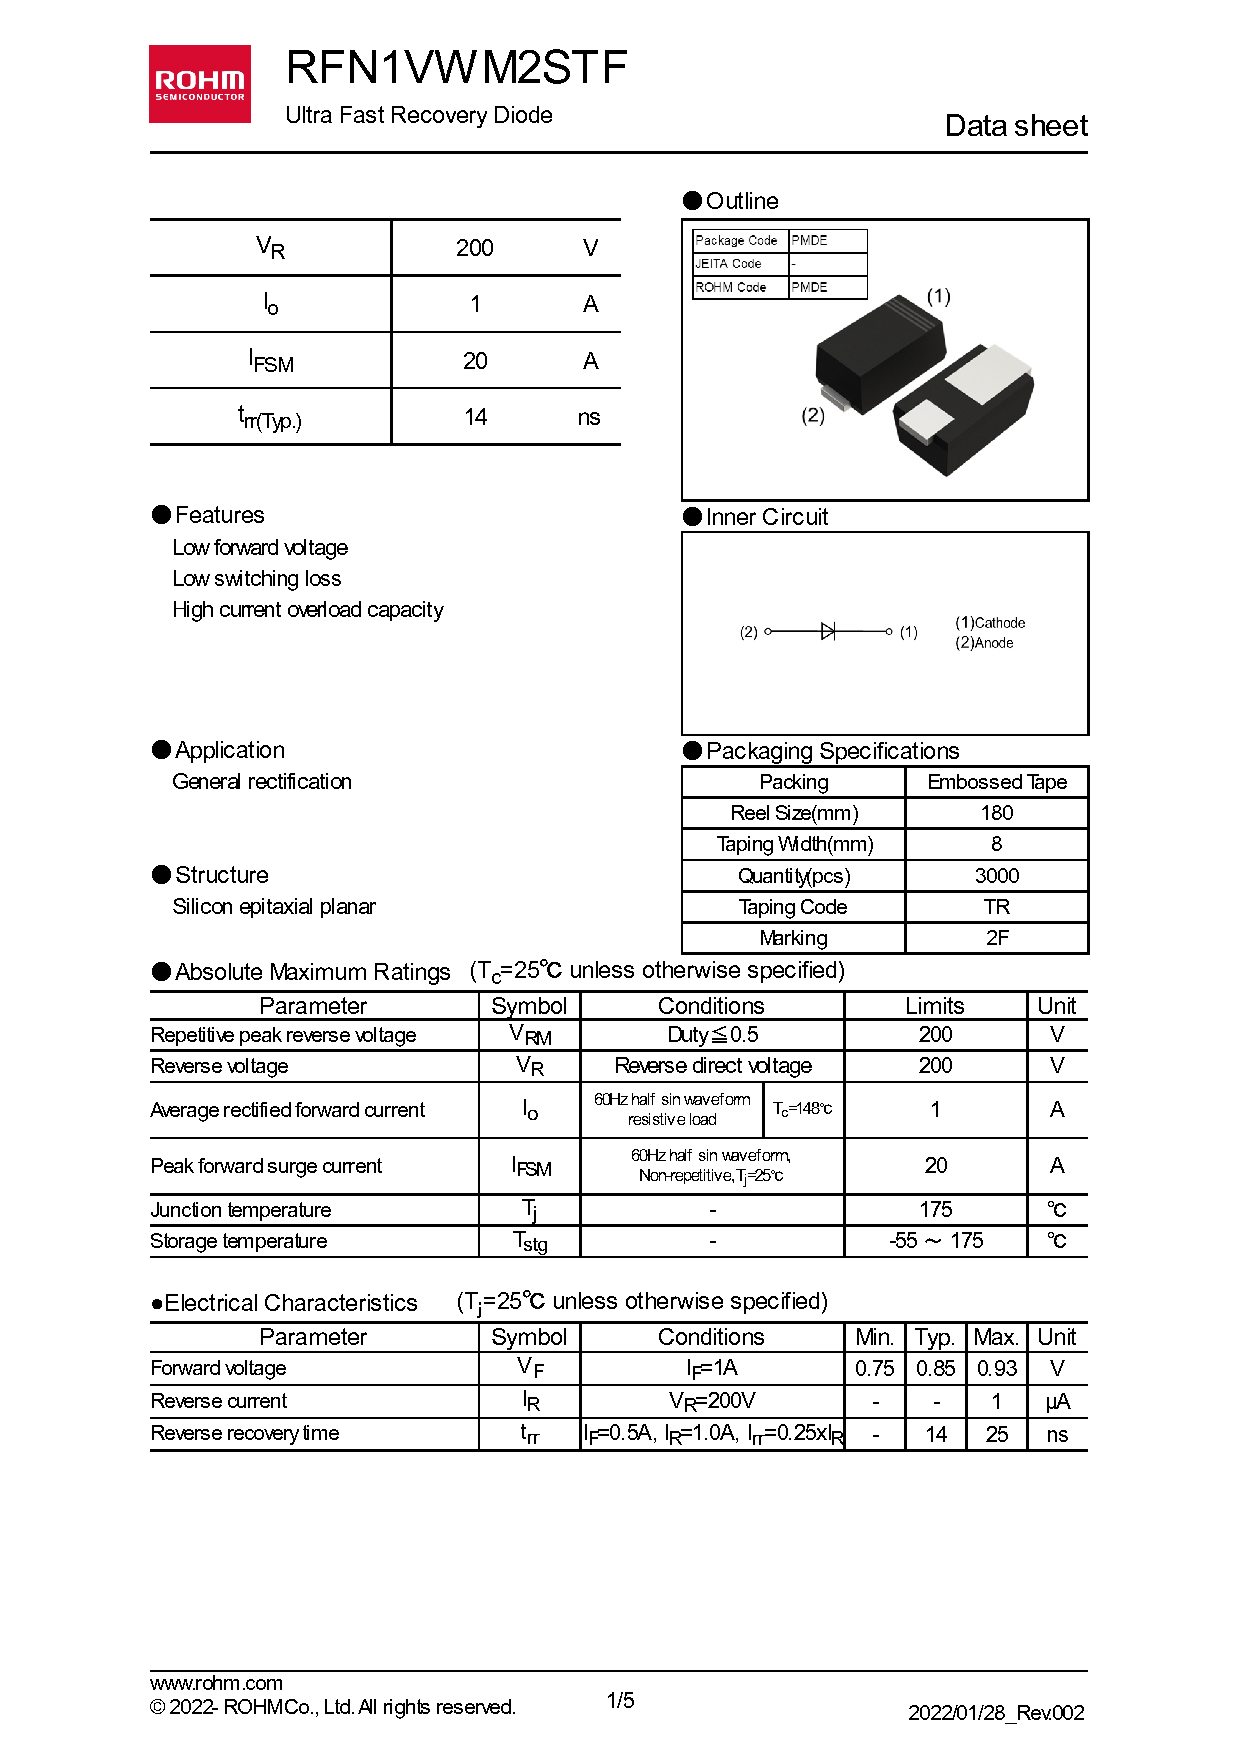
\includepdf[page=1,scale=\includepdfscale,pagecommand={\subsection{Diode Datasheet}\hypertarget{Diode}{}}]{Diode.pdf}
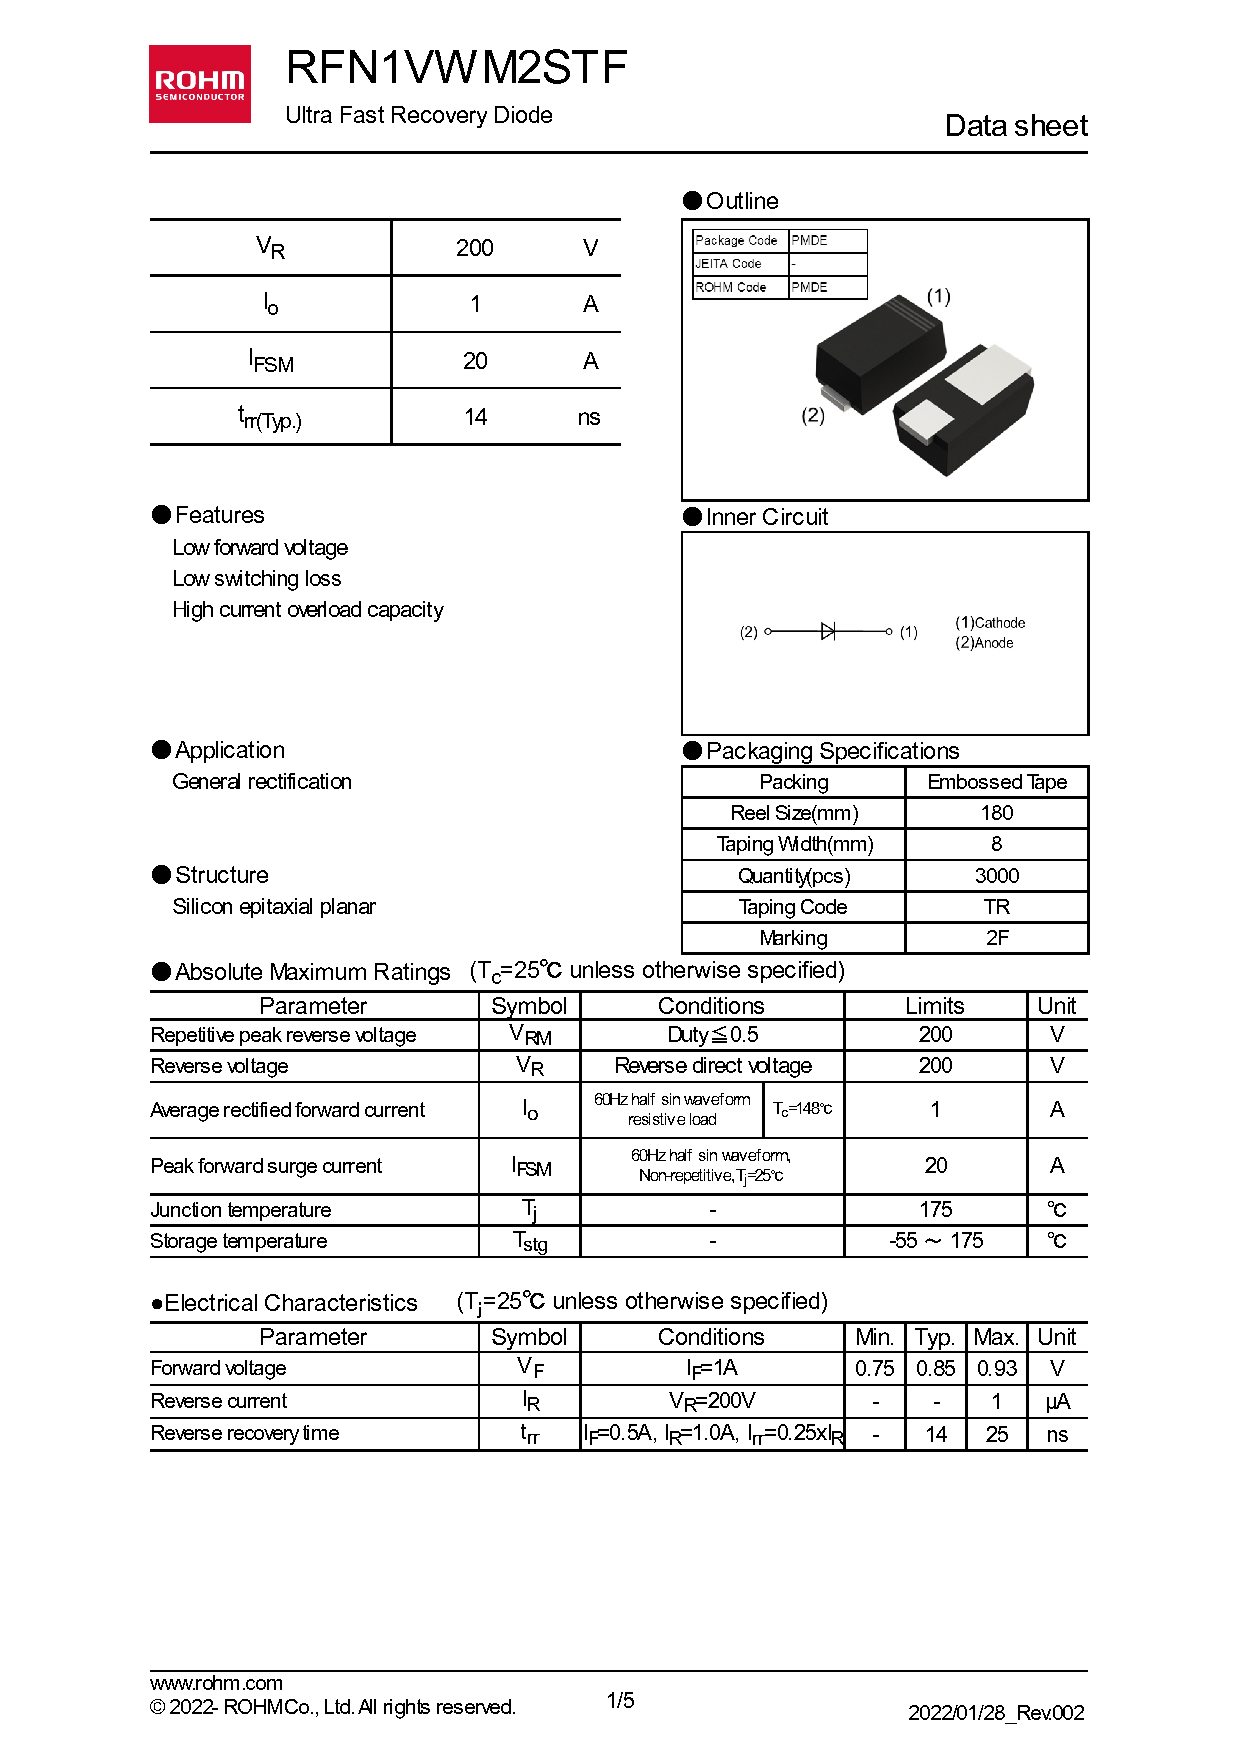
\includepdf[page=2-4,scale=\includepdfscale,pagecommand={}]{Diode.pdf}

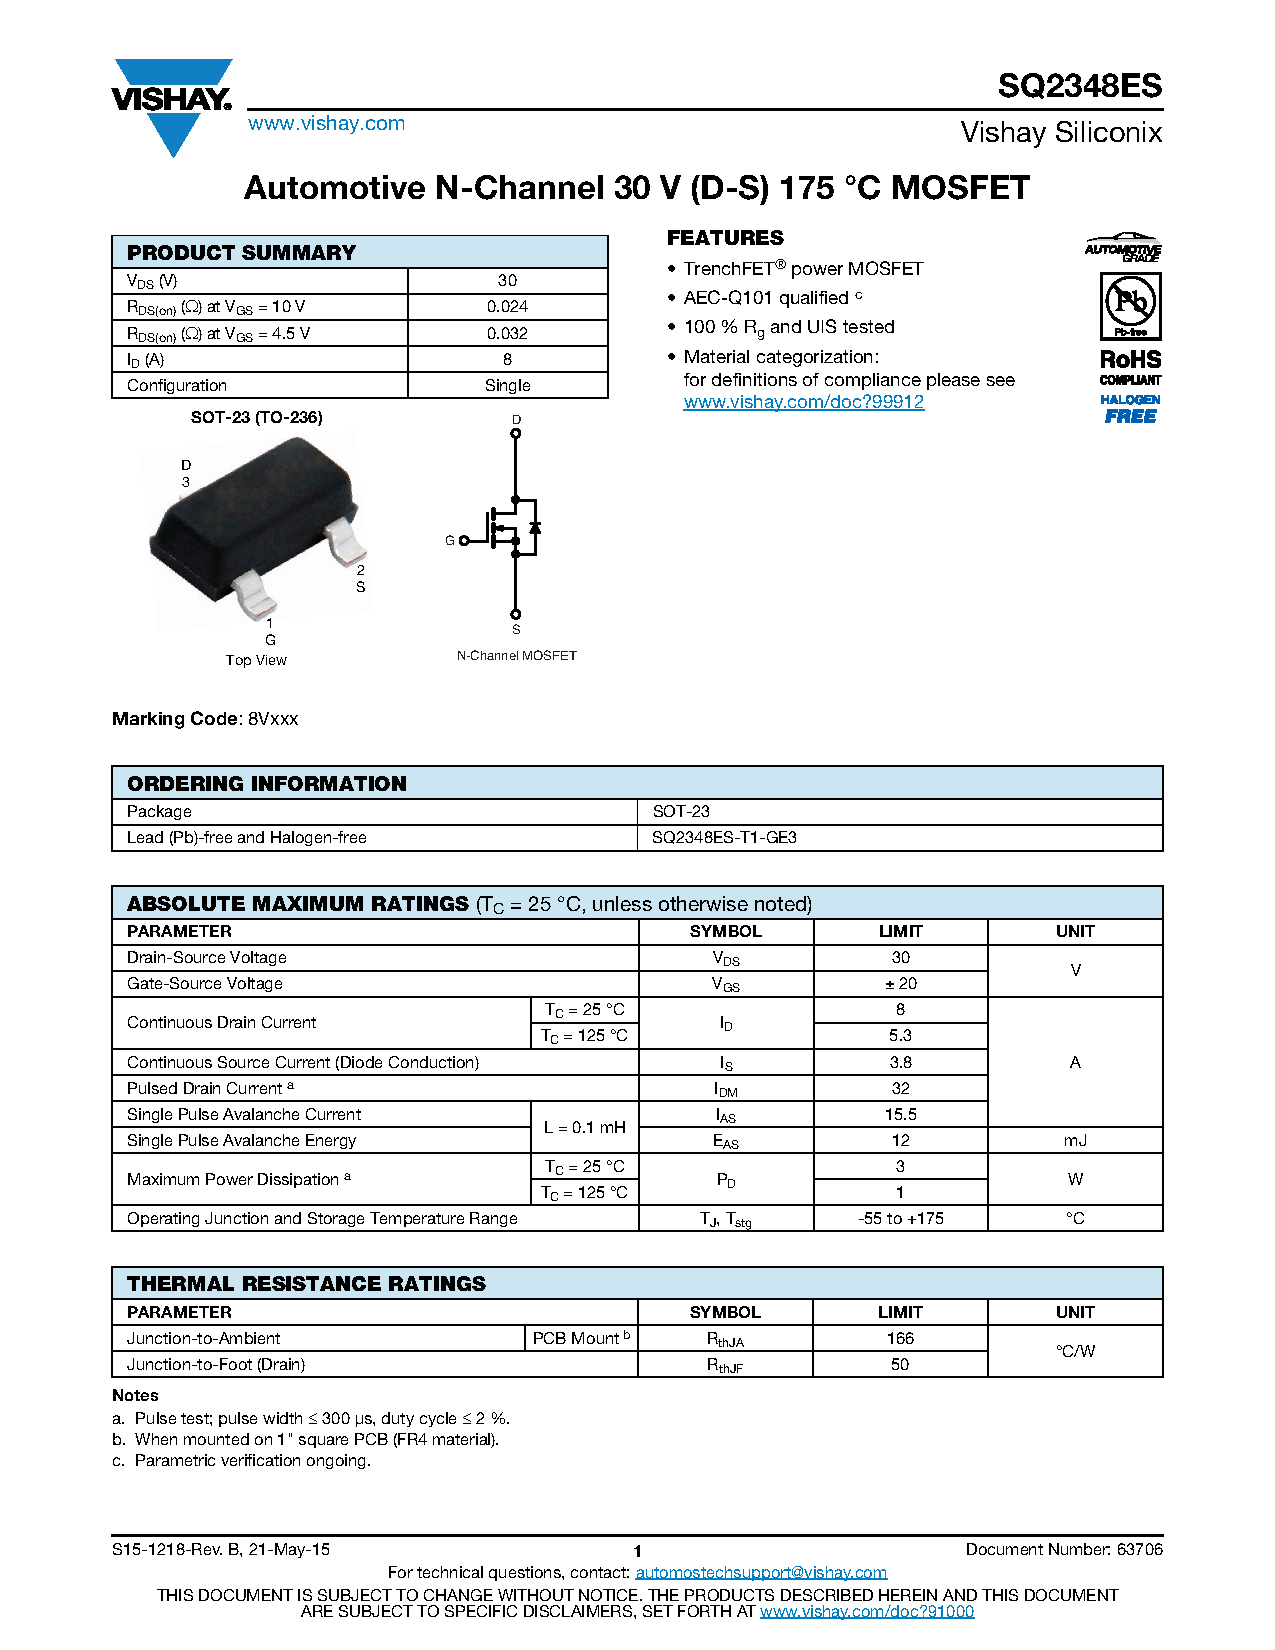
\includepdf[page=1,scale=\includepdfscale,pagecommand={\subsection{NMOS Datasheet}\hypertarget{NMOS}{}}]{NMOS.pdf}
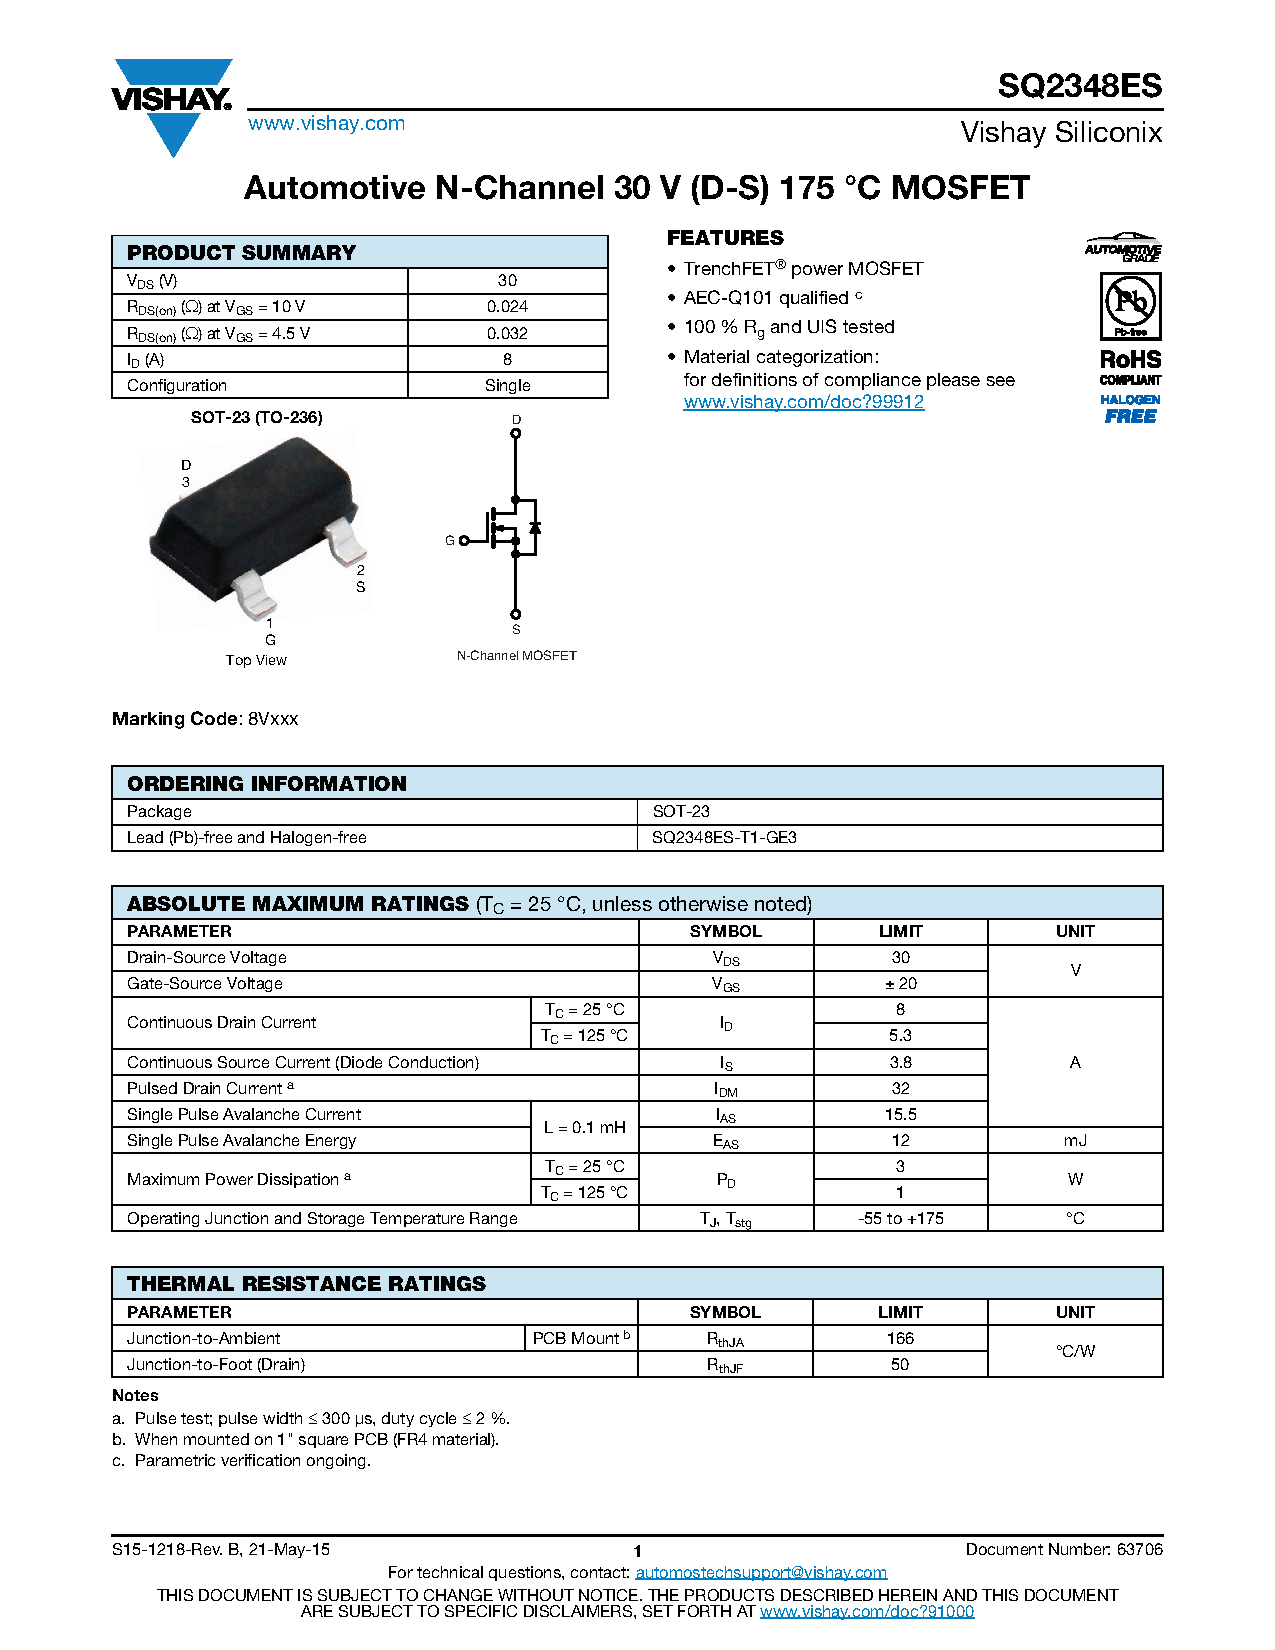
\includepdf[page=2-3,scale=\includepdfscale,pagecommand={}]{NMOS.pdf}

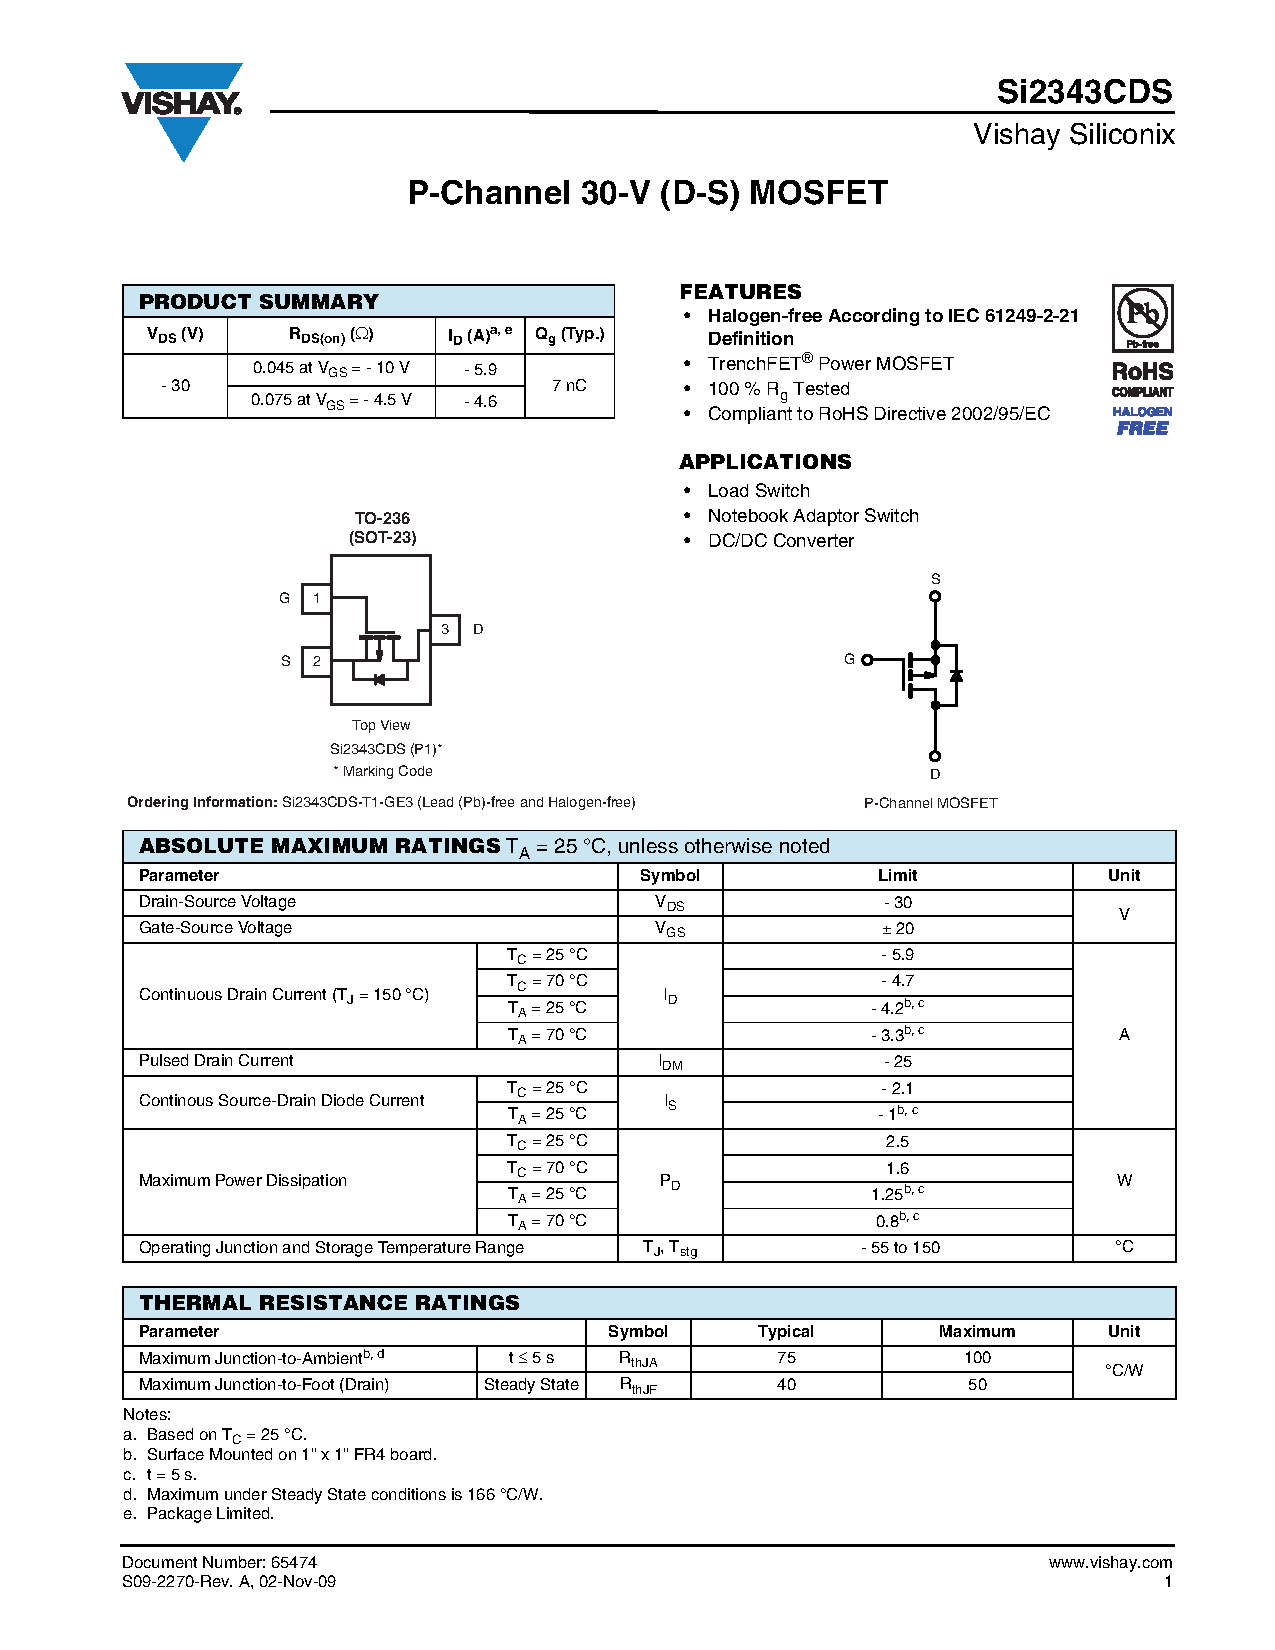
\includepdf[page=1,scale=\includepdfscale,pagecommand={\subsection{PMOS Datasheet}\hypertarget{PMOS}{}}]{PMOS.pdf}
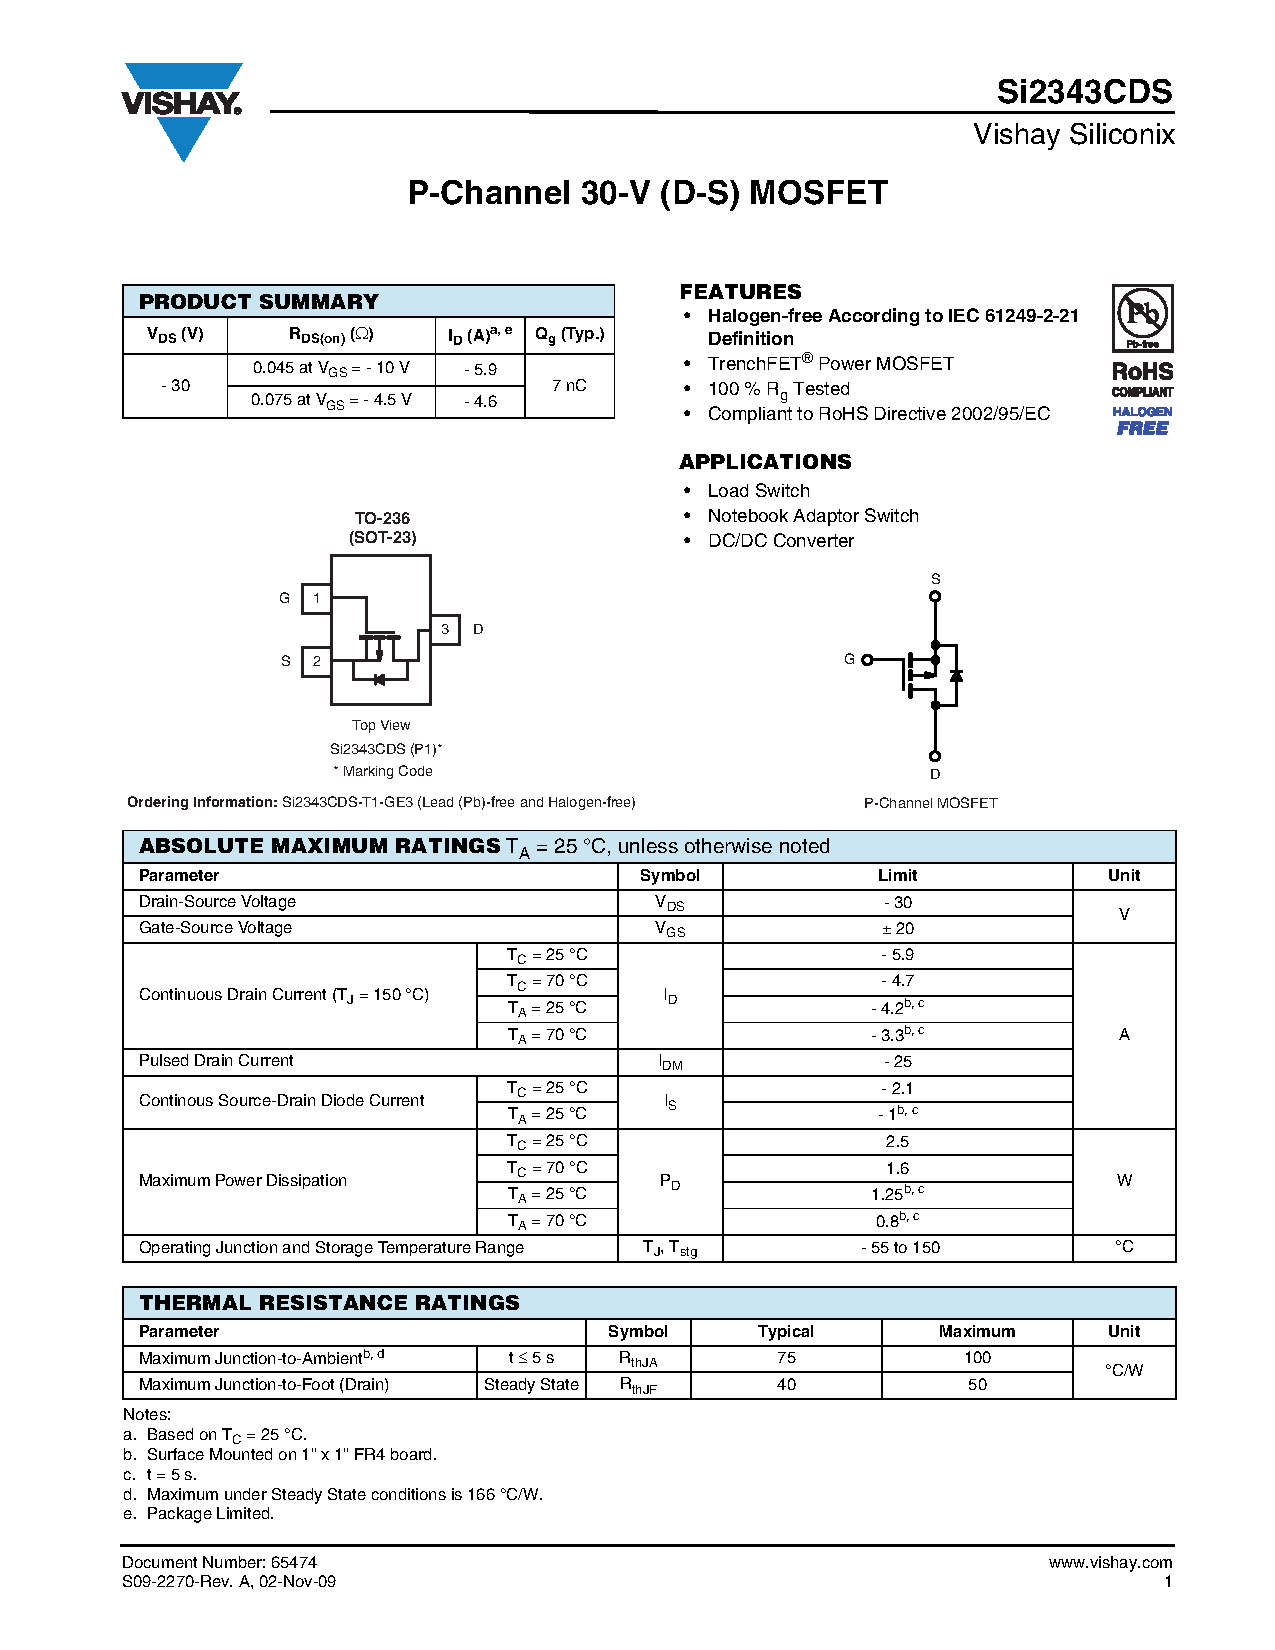
\includepdf[page=2-6,scale=\includepdfscale,pagecommand={}]{PMOS.pdf}

\end{document}